%\documentclass[twoside]{article}

\documentclass[accepted]{uai2023}

% \documentclass[11pt]{article}


% % Fonts
% \usepackage{palatino}
% \linespread{1.05}			% Palatino needs more leading (space between lines)
% \usepackage{times}
% %\usepackage{mathpazo}		% use [sc] option for more line spacing
% %\usepackage[T1]{fontenc}
% % End Fonts

% \usepackage[letterpaper,margin=1in]{geometry}
% %\usepackage[margin=1.0in]{geometry}

% \setlength{\parskip}{4pt}
% \setlength{\parindent}{0pt}

\usepackage[utf8]{inputenc} % allow utf-8 input
\usepackage[T1]{fontenc}    % use 8-bit T1 fonts
\usepackage{hyperref}       % hyperlinks
\usepackage{amsfonts,amsmath,amssymb,amsthm}       % blackboard math symbols
\usepackage{array}
%\usepackage{subcaption}
\usepackage{url}            % simple URL typesetting
\usepackage{booktabs}       % professional-quality tables
\usepackage{nicefrac}       % compact symbols for 1/2, etc.
\usepackage{microtype}      % microtypography
\usepackage[dvipsnames]{xcolor}         % colors
\usepackage{bm}

%\usepackage{natbib}
\usepackage[round]{natbib}
\renewcommand{\bibname}{References}
\renewcommand{\bibsection}{\subsubsection*{\bibname}}

\usepackage{graphicx}
\usepackage{subfigure}
%\usepackage{booktabs}
\usepackage{hyperref}
% Attempt to make hyperref and algorithmic work together better:
%\newcommand{\theHalgorithm}{\arabic{algorithm}}

\usepackage{bigints}
\usepackage{amssymb,amsopn,algorithm,algorithmic,float,bbm,bm,enumerate,color,multirow,gensymb}
%\usepackage{algpseudocode} %
%\renewcommand{\algorithmicrequire}{\textbf{Input:}}
%\renewcommand{\algorithmicensure}{\textbf{Output:}}

\usepackage{epsfig,subfigure,graphicx}

\usepackage{comment}
%\usepackage[dvipsnames]{xcolor}
%\usepackage{authblk}
\usepackage{afterpage}
\usepackage{thmtools,thm-restate}


\newcommand{\beq}{\begin{equation}}
\newcommand{\eeq}{\end{equation}}

\newcommand{\htn}{\hat{\theta}_{\lambda_n}}
\newcommand{\hdn}{\hat{\Delta}_n}

\newcommand{\mr}[1]{\textcolor{red}{#1}}
\newcommand{\mb}[1]{\textcolor{blue}{#1}}

\newcommand\norm[1]{\left\lVert#1\right\rVert}
\renewcommand\vec[1]{\operatorname{vec}#1}


%% ========================================================
\newcommand\B{\mathbb{B}}
\newcommand\E{\mathbb{E}}
\renewcommand\P{\mathbb{P}}
\newcommand\I{\mathbb{I}}
\newcommand\N{\mathbb{N}}
\newcommand\s{\mathbb{S}}
\newcommand\R{\mathbb{R}}
\newcommand\W{\mathbb{W}}
\newcommand\X{\mathbb{X}}
\newcommand\Y{\mathbb{Y}}

\newcommand\1{\mathbbm{1}}
\newcommand\0{\mathbbm{0}}

\newcommand{\bz}{\mathbf{0}}
\newcommand{\bo}{\mathbf{1}}

\newenvironment{packed_enum}{
\begin{enumerate}
  \setlength{\itemsep}{1pt}
  \setlength{\parskip}{0pt}
  \setlength{\parsep}{0pt}
}{\end{enumerate}}

%% ========================================================
%% Some useful commands. Note the dangerous \r command!
%% ========================================================



\newcommand{\bd}{\boldsymbol}
\newcommand{\mf}{\mathbf}


\newcommand{\g}{\mathbf{g}}



\renewcommand{\a}{\mathbf{a}}
\renewcommand{\b}{\mathbf{b}}
\renewcommand{\c}{\mathbf{c}}
\newcommand{\f}{\mathbf{f}}
\renewcommand{\r}{\mathbf{r}} % since \r was already defined in altex
\renewcommand{\u}{\mathbf{u}}
\renewcommand{\v}{\mathbf{v}}
\newcommand{\V}{\mathbf{V}}
\newcommand{\es}{\mathbf{s}}
\newcommand{\w}{\mathbf{w}}
\newcommand{\x}{\mathbf{x}}
\newcommand{\y}{\mathbf{y}}
\newcommand{\z}{\mathbf{z}}
\newcommand{\p}{\mathbf{p}}
\newcommand{\q}{\mathbf{q}}
\renewcommand{\I}{\mathbb{I}}




%----------------------------------------
%      THE SETS
%----------------------------------------
\newcommand{\cC}{{\cal C}}
\newcommand{\cH}{{\cal H}}
\newcommand{\cI}{{\cal I}}
\newcommand{\cL}{{\cal L}}
\newcommand{\cM}{{\cal M}}
%\newcommand{\M}{\mathcal{M}}
\newcommand{\cN}{{\cal N}}
\newcommand{\cP}{{\cal P}}
\newcommand{\cQ}{{\cal Q}}
\newcommand{\cS}{{\cal S}}
\newcommand{\cT}{{\cal T}}
\newcommand{\cW}{{\cal W}}
\newcommand{\cX}{{\cal X}}
\newcommand{\cY}{{\cal Y}}
\newcommand{\cF}{{\cal F}}
\newcommand{\cZ}{{\cal Z}}

\newcommand{\cA}{{\cal A}}
\newcommand{\cB}{{\cal B}}
\newcommand{\cD}{{\cal D}}
\newcommand{\cG}{{\cal G}}
\newcommand{\cE}{{\cal E}}


%--------------------------------------------
%         THE VARIABLES & APPROXIMATES
%--------------------------------------------

% Bold variables for vectors, matrices
\newcommand{\bA}{\mathbf{A}}
\newcommand{\bB}{\mathbf{B}}
\newcommand{\bC}{\mathbf{C}}
\newcommand{\bD}{\mathbf{D}}
\newcommand{\bE}{\mathbf{E}}
\newcommand{\bI}{\mathbf{I}}
\newcommand{\bM}{\mathbf{M}}
\newcommand{\bR}{\mathbf{R}}
\newcommand{\bU}{\mathbf{U}}
\newcommand{\bV}{\mathbf{V}}
\newcommand{\bW}{\mathbf{W}}
\newcommand{\bX}{\mathbf{X}}
\newcommand{\bY}{\mathbf{Y}}
%\newcommand{\bZ}{\mathbf{Z}}

\newcommand{\bgg}{\mathbf{g}}

%\newcommand{\bz}{\mathbf{z}}
\newcommand{\hZ}{\hat{Z}}
\newcommand{\hbZ}{\hat{\bZ}}
\newcommand{\hz}{\hat{z}}

\newcommand{\hU}{\hat{U}}
\newcommand{\hV}{\hat{V}}
\newcommand{\hu}{\hat{u}}
\newcommand{\hv}{\hat{v}}


\newcommand{\hX}{\hat{X}}
\newcommand{\hY}{\hat{Y}}
\newcommand{\hatx}{{\hat{x}}}
\newcommand{\haty}{{\hat{y}}}

%---------MISC-----------------------------



\newcommand{\m}{\boldsymbol{\mu}}
\newcommand{\bmu}{\boldsymbol{\mu}}
\newcommand{\llambda}{\boldsymbol{\lambda}}
\newcommand{\bchi}{\boldsymbol{\chi}}
\newcommand{\btheta}{\boldsymbol{\theta}}
\newcommand{\Eta}{\boldsymbol{\eta}}
\newcommand{\oomega}{\boldsymbol{\omega}}
\newcommand{\ppi}{\boldsymbol{\pi}}
\newcommand{\pphi}{\boldsymbol{\phi}}
\newcommand{\ggamma}{\boldsymbol{\gamma}}
\newcommand{\bbeta}{\boldsymbol{\beta}}
\newcommand{\aalpha}{\boldsymbol{\alpha}}
\newcommand{\eepsilon}{\boldsymbol{\epsilon}}

\newcommand{\bxi}{\boldsymbol{\xi}}
\newcommand{\bzeta}{\boldsymbol{\zeta}}
\newcommand{\beeta}{\boldsymbol{\eta}}

%\newcommand{\norm}[2]{\ensuremath \|#1\|_{#2}}
\newcommand{\no}[1]{\norm{#1}{}}
\newcommand{\myref}[1]{(\ref{#1})}
\newcommand{\del}[2]{\frac{\partial #1}{\partial #2}}


%----------------------------------------------
%        NEW OPERATORS
%----------------------------------------------
\DeclareMathOperator{\argsup}{argsup}
\DeclareMathOperator{\arginf}{arginf}
\DeclareMathOperator{\argmax}{argmax}
\DeclareMathOperator{\argmin}{argmin}
\DeclareMathOperator{\avg}{avg}
\DeclareMathOperator{\Int}{int}
\DeclareMathOperator{\cl}{cl}
\DeclareMathOperator{\bnd}{bd}
\DeclareMathOperator{\epi}{epi}
\DeclareMathOperator{\dom}{dom}
\DeclareMathOperator{\ri}{ri}
\DeclareMathOperator{\co}{co}
\DeclareMathOperator{\sgn}{sign}
\DeclareMathOperator{\supp}{supp}
\DeclareMathOperator{\discrete}{Discrete}
\DeclareMathOperator{\gam}{GAM}
\DeclareMathOperator{\uni}{Uniform}
\DeclareMathOperator{\dir}{Dir}
\DeclareMathOperator{\gaam}{GAM}
\DeclareMathOperator{\Beta}{Beta}
\DeclareMathOperator{\tr}{Tr}
\DeclareMathOperator{\cone}{cone}
\DeclareMathOperator{\gen}{gen}
\DeclareMathOperator{\lsd}{LSD}
\DeclareMathOperator{\euc}{Euc}
\DeclareMathOperator{\spec}{Spec}
\DeclareMathOperator{\diag}{diag}
\DeclareMathOperator{\poly}{poly}
\DeclareMathOperator{\polylog}{polylog}


\DeclareMathOperator{\gelu}{GELU}
\DeclareMathOperator{\erf}{erf}
\DeclareMathOperator{\ntk}{ntk}

%---------------------------------------------
% EQUATION, FIGURE, TABLE NUMBERS
%---------------------------------------------

%\renewcommand{\theequation}{\thesection.\arabic{equation}}
%\renewcommand{\thefigure}{\thesection.\arabic{figure}}
%\renewcommand{\thetable}{\thesection.\arabic{table}}
%\numberwithin{equation}{section}



%---------------------------------------------
% THEOREMS, EXAMPLES ETC.
%---------------------------------------------

% \newcounter{exampleI}
% \setcounter{exampleI}{1}
% \renewcommand{\theexampleI}{\arabic{exampleI}}

% {\theorembodyfont{\rmfamily} \theoremstyle{plain} \newtheorem{subexampleI}{Example}[exampleI]}
% \renewcommand{\thesubexampleI}{\theexampleI.\Alph{subexampleI}}

% \newcounter{exampleII}
% \setcounter{exampleII}{2}
% \renewcommand{\theexampleII}{\arabic{exampleII}}

% {\theorembodyfont{\rmfamily} \theoremstyle{plain} \newtheorem{subexampleII}{Example}[exampleII]}
% \renewcommand{\thesubexampleII}{\theexampleII.\Alph{subexampleII}}

% \newcounter{exampleIII}
% \setcounter{exampleIII}{3}
% \renewcommand{\theexampleIII}{\arabic{exampleIII}}

% {\theorembodyfont{\rmfamily} \theoremstyle{plain} \newtheorem{subexampleIII}{Example}[exampleIII]}
% \renewcommand{\thesubexampleIII}{\theexampleIII.\Alph{subexampleIII}}


%{\theorembodyfont{\rmfamily} \newtheorem{exam}{Example}}
% {\theorembodyfont{\rmfamily} \newtheorem{defn}{Definition}}
%{\theorembodyfont{\rmfamily} \newtheorem{remark}{Remark}}
\newtheorem{theo}{Theorem}[section]
\newtheorem{prop}{Proposition}[section]
\newtheorem{lemm}{Lemma}[section]
\newtheorem{corr}{Corollary}[section]
\newtheorem{clm}{Claim}
\newtheorem{asmp}{Assumption}
\newtheorem{defn}{Definition}[section]

\theoremstyle{definition} 
\newtheorem{exam}{Example}[section]
\newtheorem{remark}{Remark}[section]

% \newcommand{\proof}{\noindent{\itshape Proof:}\hspace*{1em}}
% \newcommand{\proofsketch}{\noindent{\itshape Proof Sketch:}\hspace*{1em}}
% \newcommand{\qed}{\nolinebreak[1]~~~\hspace*{\fill} \rule{5pt}{5pt}\vspace*{\parskip}\vspace*{1ex}}



\newcommand{\cx}{{\hat{x}}}
\newcommand{\cy}{{\hat{y}}}
\newcommand{\bp}{{\bar{p}}}
\newcommand{\eqn}[1]{(\ref{eq:#1})}
\newcommand {\commentout}[1] {}

%------------------------------------------

%%%%%%%%%%%Definitions and Macros

\def\ints{{{\rm Z} \kern -.35em {\rm Z} }}  % ints
\def\smallints{{{\rm Z} \kern -.3em {\rm Z} }}  % small ints
\def\pints{{{\rm I} \kern -.15em {\rm N} }}      % pints
\newcommand{\reals}{\mathbb R}
\newcommand{\integers}{\mathbb Z}

\newcommand{\lapn}{\lessapprox_{\,n}}
\newcommand{\gapn}{\gtrapprox_{\,n}}
\newcommand{\apn}{\approx_n}

%\def\reals{{{\rm I} \kern -.2em {\rm R} }} % reals
\newcommand{\RR}{\mathbb R}
\def\cplx{{{\rm I} \kern -.45em {\rm C} }}       % complex
\def\l2{\rm {\mathcal L}^{2}(\reals)}            % l2

\newcommand{\seqz}[2]{\mbox{$\{#1_{#2}\}$}_{#2 \in \smallints }}
\newcommand{\seqn}[2]{\mbox{$\{#1_{#2}\}$}_{#2 \in \pints }}
%\renewcommand{\norm}[1]{\lVert#1\rVert}
\newcommand{\abs}[1]{\left|#1\right|}


\newtheorem{problem}{Problem}
\newtheorem{definition}{Definition}[section]
\newtheorem{nad}{Notation and Definitions}[section]
\newtheorem{notation}{Notation}[section]
%\newtheorem{remark}{Remark}[section]
\newtheorem{theorem}{Theorem}[section]
\newtheorem{lemma}[theorem]{Lemma}
\newtheorem{claim}{Claim}[theorem]
\newtheorem{proposition}{Proposition}[section]
\newtheorem{corollary}{Corollary}
\newtheorem{example}{Example}
\newtheorem{conjecture}{Conjecture}
%\newtheorem{algorithm}{Algorithm}
\newtheorem{exercise}{Exercise}
\newtheorem{step}{Step}

\newcommand{\nr}{\nonumber}
\newcommand{\be}{\begin{eqnarray}}
\newcommand{\ee}{\end{eqnarray}}
\newcommand{\bea}{\begin{eqnarray}}
\newcommand{\eea}{\end{eqnarray}}
\newcommand{\beaa}{\begin{eqnarray*}}
\newcommand{\eeaa}{\end{eqnarray*}}
\newcommand{\bnad}{\begin{nad}}
\newcommand{\enad}{\end{nad}}


\newcommand{\gb}{\beta_{\infty}}
\newcommand{\mgb}{\tilde{\beta}_{\infty}}
\newcommand{\gbb}{\beta_{2}}
\newcommand{\mgbb}{\tilde{\beta}_{2}}
\newcommand{\Jf}{J_{\infty}}
\newcommand{\mmJf}{\overline{J}_{\infty}}
\newcommand{\mJf}{\tilde{J}_{\infty}}
\newcommand{\Jff}{J_{2}}
\newcommand{\mJff}{\tilde{J}_{2}}
\newcommand{\Jc}{{\calJ_{\infty}}}
\newcommand{\mJc}{{\tilde{\calJ}_{\infty}}}
\newcommand{\Jcc}{{\calJ_{2}}}
\newcommand{\ptq}{P_{3 \overline{Q}}}
\newcommand{\pq}{P_{Q}}


\newcommand{\di}{{\,\mathrm{d}}}
\newcommand{\latop}[2]{\genfrac{}{}{0pt}{}{#1}{#2}}


%\newcommand{\Th}[1]{Theorem~\ref{#1}} % when starting a sentence
%\renewcommand{\th}[1]{Theorem~\ref{#1}}
%\newcommand{\ths}[2]{Theorems~\ref{#1} and~\ref{#2}}
%\newcommand{\thst}[2]{Theorems~\ref{#1}-\ref{#2}}
%\newcommand{\lem}[1]{Lemma~\ref{#1}}
%\newcommand{\prop}[1]{Proposition~\ref{#1}}
%\newcommand{\defin}[1]{Definition~\ref{#1}}
%\newcommand{\eq}[1]{equation~(\ref{#1})}
%\newcommand{\ineq}[1]{inequality~(\ref{#1})}
%\newcommand{\Ineq}[1]{Inequality~(\ref{#1})}
%\newcommand{\ineqs}[2]{inequalities~(\ref{#1}) and~(\ref{#2})}
%\newcommand{\Eq}[1]{Equation~(\ref{#1})}
%\newcommand{\eqs}[2]{equations~(\ref{#1}) and~(\ref{#2})}
%\newcommand{\eqss}[3]{equations~(\ref{#1}), (\ref{#2}) and~(\ref{#3})}
%\newcommand{\eqst}[2]{equations~(\ref{#1})-(\ref{#2})}
%\newcommand{\sect}[1]{Section~\ref{#1}}
%\newcommand{\subsect}[1]{Subsection~\ref{#1}}

\newcommand{\lip}{\langle}
\newcommand{\rip}{\rangle}
\newcommand{\uu}{\underline}
\newcommand{\oo}{\overline}
\newcommand{\La}{\Lambda}
\newcommand{\la}{\lambda}
%\newcommand{\eps}{\epsilon}
\newcommand{\eps}{\varepsilon}
\newcommand{\veps}{\varepsilon}
\newcommand{\rmT}{{\rm T}}
\newcommand{\rmW}{{\rm W}}
\newcommand{\Ga}{\Gamma}

\newcommand{\sign}{{\mbox{\rm sign}}}
\newcommand{\ang}{{\mbox{\rm ang}}}
%\newcommand{\supp}{{\mbox{\rm supp}}}
\newcommand{\dist}{{\mbox{\rm dist}}}

\newcommand{\nin}{\in\!\!\!\!\!/\,}

\newcommand{\calA}{{\cal A}}
\newcommand{\calB}{{\cal B}}
\newcommand{\calC}{{\cal C}}
\newcommand{\calD}{{\cal D}}
\newcommand{\tcD}{{\tilde{\cal D}}}
\newcommand{\calE}{{\cal E}}
\newcommand{\calF}{{\cal F}}
\newcommand{\calG}{{\cal G}}
\newcommand{\calH}{{\cal H}}
\newcommand{\calI}{{\cal I}}
\newcommand{\calJ}{{\cal J}}
\newcommand{\calK}{{\cal K}}
\newcommand{\calL}{{\cal L}}
\newcommand{\calM}{{\cal M}}
\newcommand{\calN}{{\cal N}}
\newcommand{\calO}{{\cal O}}
\newcommand{\calP}{{\cal P}}
\newcommand{\calQ}{{\cal Q}}
\newcommand{\calR}{{\cal R}}
\newcommand{\calS}{{\cal S}}
\newcommand{\calT}{{\cal T}}
\newcommand{\calU}{{\cal U}}
\newcommand{\calV}{{\cal V}}
\newcommand{\calW}{{\cal W}}
\newcommand{\calX}{{\cal X}}
\newcommand{\calY}{{\cal Y}}
\newcommand{\calZ}{{\cal Z}}

\newcommand{\RE}{{\cal R}e}
%\newcommand{\IM}{{\cal I}m}


\newcommand{\Prob}{{\rm Prob\,}}
\newcommand{\diam}{{\rm diam\,}}
\renewcommand{\mod}{{\rm mod\,}}
\newcommand{\sinc}{{\rm sinc\,}}
\newcommand{\ctg}{{\rm ctg\,}}
\newcommand{\ifff}{\mbox{\ if and only if\ }}
%\newcommand{\proof}{\noindent {\bf Proof:\ }}

% %\renewcommand{\bar}{\overline}
% \renewcommand{\overline}{\bar}
% %\renewcommand{\tilde}{\widetilde}
% \renewcommand{\widetilde}{\tilde}
% %\renewcommand{\ell}{l}
% %\renewcommand{\hat}{\widehat}
% \renewcommand{\widehat}{\hat}






\usepackage[dvipsnames]{xcolor}
%\usepackage[]{color-edits}
\usepackage[suppress]{color-edits}
\addauthor{ab}{violet}
\addauthor{abg}{green}
\addauthor{pc}{red}
\addauthor{mb}{magenta}
\addauthor{lz}{teal}

\newcommand\pc[1]{\textcolor{red}{#1}} %Pedro's highlights 
%\newcommand\ab[1]{\textcolor{blue}{#1}} %Arindam's highlights


% \title{Deep Learning Optimization with Smooth Activations:\\Linear Width Suffices for the NTK condition}


% The \author macro works with any number of authors. There are two commands
% used to separate the names and addresses of multiple authors: \And and \AND.
%
% Using \And between authors leaves it to LaTeX to determine where to break the
% lines. Using \AND forces a line break at that point. So, if LaTeX puts 3 of 4
% authors names on the first line, and the last on the second line, try using
% \AND instead of \And before the third author name.
%\bibliographystyle{plainnat}
\renewcommand{\bibsection}{\subsubsection*{References}}


%\tile{Deep Learning Optimization with Smooth Activations:\\Linear Width Suffices}
\title{Neural Tangent Kernel at Initialization: Linear Width Suffices}

%\aistatstitle{Deep Learning Optimization with Smooth Activations:\\Linear Width Suffices for the NTK condition}

% Add authors
\author[1]{\href{mailto:<arindamb@illinois.edu>?Subject=Your UAI 2023 paper}
{Arindam Banerjee}{}}
\author[1]{\href{mailto:<pacisne@gmail.com>?Subject=Your UAI 2023 paper}{Pedro Cisneros-Velarde}{}}
\author[2]{\href{mailto:<l5zhu@ucsd.edu>?Subject=Your UAI 2023 paper}{Libin Zhu}{}}
\author[2]{\href{mailto:<mbelkin@ucsd.edu>?Subject=Your UAI 2023 paper}{Mikhail Belkin}{}}
\affil[1]{University of Illinois at Urbana-Champaign}
\affil[2]{University of California, San Diego}
% Department of Computer Science\\
% Halicioğlu Data Science Institute\\
%University of California, San Diego\\



% \author{%
% %\hspace*{-10mm}
%   Arindam Banerjee \\ 
%   Department of Computer Science\\
%   University of Illinois  Urbana-Champaign\\
%   \texttt{arindamb@illinois.edu} \\
%   \and
%   Pedro Cisneros-Velarde\\
%     Department of Computer Science\\
%     \hspace*{-5mm} University of Illinois Urbana-Champaign\\
%     \texttt{pacisne@gmail.com}
%   \and
%     Libin Zhu\\
%     Department of Computer Science\\
%     University of California, San Diego\\
%     \texttt{l5zhu@ucsd.edu}
%     \and
%     Mikhail Belkin\\ 
%     Halicioglu Data Science Institute\\
%     University of California, San Diego\\
%     \texttt{mbelkin@ucsd.edu}
% } 

% \maketitle

\begin{document}
\maketitle

\begin{abstract}
In this paper we study the problem of lower bounding the minimum eigenvalue of the neural tangent kernel (NTK) at initialization, an important quantity for the theoretical analysis of training in neural networks. We consider feedforward neural networks with smooth activation functions.
\abedit{Without any distributional assumptions on the input,} we present a novel result: we show that 
for suitable initialization variance, $\widetilde{\Omega}(n)$ width, where $n$ is the number of training samples, suffices to ensure that the NTK at initialization is positive definite, improving prior results for smooth activations under our setting. 
\pcedit{Prior to our work, the sufficiency of linear width has only been shown either for networks with ReLU activation functions, and sublinear width has been shown for smooth networks but with additional conditions on the distribution of the data.} \abedit{The technical challenge in the analysis stems from the layerwise inhomogeneity of smooth activation functions and we handle the challenge using {\em generalized} Hermite series expansion of such activations.}
\end{abstract}


\section{INTRODUCTION}
\label{sec:arXiv_intro}

%\abcomment{update} 
Recent  years have seen advances in understanding convergence of gradient descent (GD) and variants for the training of deep learning models~\citep{SD-JL-HL-LW-XZ:19,ZAZ-YL-ZS:19,DZ-QG:19,DZ-YC-DZ-QG:20,CL-LZ-MB:21,ZJ-MT:19,oymak2020hermite,ng2021opt}. Despite the fact that such optimization problems are non-convex, a series of recent results have shown that GD has geometric convergence and finds near global solution "near initialization" for wide networks. Such analysis is typically done based on the Neural Tangent Kernel (NTK)~\citep{AJ-FG-CH:18}. The NTK is positive definite "near initialization," the optimization problem then satisfies a condition closely related to the Polyak-Łojasiewicz (PL) condition, which in turn implies geometric convergence to the global minima~\citep{CL-LZ-MB:21,ng2021opt}. A very important step in the analysis is to derive a condition 
% lower bound 
on the required network's width to ensure the \emph{NTK condition} is satisfied at initialization, i.e., that the minimum eigenvalue of the NTK is lower bounded at initialization by a positive constant.
%The larger such eigenvalue is, the better the convergence properties of the algorithm.\pccomment{Not sure if this last sentence is correctly stated.}
\pcdelete{Such results have been generalized to more flexible forms of "lazy learning" where similar guarantees hold~\citep{LC-EO-FB:19}. However, there are  questions regarding whether such "near initialization" or "lazy learning" truly explains the optimization behavior in realistic deep learning models~\citep{MG-SS-AJ-MW:20,GY-EJH:20,SF-GKD-MP-SK-DR-SG:20,LC-EO-FB:19}.
%\mbcomment{do we claim to explain optimization in realistic models though?} \abcomment{perhaps not, but we relax the "near initialization" part, and get to PL through RSC, not NTK}
}

Much of the theoretical convergence analysis of deep models has focused on ReLU networks~\citep{ZAZ-YL-ZS:19,ng2021opt}. While handling the non-smoothness of ReLU activation presents unique challenges, the homogeneity of ReLU helps the analysis~\citep{ZJ-MT:19,DZ-QG:19,DZ-YC-DZ-QG:20,ZAZ-YL-ZS:19,ng2020hermite1,ng2021hermite2}. On the other hand, some progress has also been made for deep models with smooth activations, where such homogeneity property does not generally hold~\citep{SD-JL-HL-LW-XZ:19,JH-HY:20}. However, many existing results for smooth networks have a high requirement on the width of the models; e.g., as polynomial powers of the number of training samples~\citep{SD-JL-HL-LW-XZ:19}. \pcedit{Recently~\cite{bombari2022memorization} have shown sublinear width on the number of training samples; however, they do require additional assumptions on the nature of the input data such as (i) scaling on the first two moments and on a variance-related quantity, as well as a (ii) Lipschitz concentration assumption on the distribution.} 
%
%\pcedit{In particular, for models with $L=O(1)$ layers, existing results need $m = \widetilde{\Omega}(n^2)$  for NTK at initialization to be positive definite for smooth actiavtions~\citep{SD-JL-HL-LW-XZ:19}.}
%Also, 
%\abdelete{existing analysis are often rather technical, and there is limited clarity on the tools for handling multiple layers of inhomogeneous activations. }
%\mbcomment{I feel it is a bit negative} \abcomment{fair concern, dropped the last bit}
%\mbcomment{I still feel that "near initialization" aspect is emphasized too much, given that our is not obviously "far from initialization"}\abcomment{the Hessian and RSC analysis allows the layerwise spectral norm radius to be $\rho < \sqrt{m}$, which is arguably much higher than what realistic deep models use}

Consider a feedforward neural network model with $L$ hidden layers of width $m$, and $\sigma_0^2$ initialization variance; trained with $n$ samples. Recent literature indicates that the NTK condition at initialization for deep networks: (i)  requires $m=\tilde{\Omega}(n)$ with ReLU activation functions~\citep{ng2021hermite2}; (ii) and for smooth activation functions requires $m = \Omega(\sqrt{n})$ under some distributional assumptions on the input data~\citep{bombari2022memorization} and $m = \Omega(n^2)$ without such assumptions~\citep{SD-JL-HL-LW-XZ:19}. Then, the motivating question for our work is: can we improve the dependence to linear width for smooth activation functions under different or weaker assumptions than distributional ones? 

\pcdelete{Then, the motivating question for our work is: since the satisfaction of the NTK condition at initialization for deep networks with ReLU activation functions~\citep{ng2021hermite2} \pcedit{or smooth activation functions with various distributional assumptions on the  input data~\citep{bombari2022memorization}} \lzcomment{I think they need $m = \Omega(\sqrt{n})$} have been recently shown to require $m=\tilde{\Omega}(n)$, can we obtain the same dependence, i.e., sufficiency of linear width, for smooth activation functions \pcedit{under different or weaker assumptions?} 
}

Our main contribution is to illustrate that $m = \widetilde{\Omega}(n)$ suffices for the NTK condition at initialization without strictly requiring additional assumptions on the distribution of the input data, \pcedit{such as the data distribution conditions stipulated in~\citep{bombari2022memorization}. Instead, our analysis relies on a basic data scaling assumption and other algebraic or geometric conditions present in the existing literature (see Remark~\ref{rem:lambda1}).\lzcomment{Do we assume data separability? If so, we should list that as one of the assumptions} However, our work assumes a neural network where all the layers have the same width, whereas \cite{bombari2022memorization} consider a challenging pyramidal topology since they study the question of achieving the minimum possible over-parameterization in neural networks.}

Our analysis builds on prior work on ReLU networks based on Hermite series expansions~\citep{oymak2020hermite,ng2020hermite1,ng2021hermite2}, which however critically relies on the homogeneity of ReLU activations. We substantially generalize such analysis to handle the inhomogeneity of multiple layers of smooth activations based on \emph{generalized} Hermite series expansions, yielding the desired sharper result. 
%\pcedit{To the best of our knowledge, our lower bound with effective linear width has only been shown to hold for ReLU networks~\citep{ng2021hermite2}.} 
\pcedit{To the best of our knowledge, our work is the first in using this mathematical framework in the analysis of neural networks.}
Our analysis extends to general depth on the network, but does not improve depth dependence of prior work~\citep{SD-JL-HL-LW-XZ:19}.
%
\pcedit{We also remark that our analysis technique is of a different nature than the one by~\citep{bombari2022memorization}, since they use tools such as restricted isometry properties for random matrices.}

Finally, our analysis \pcedit{also} reveals a possible trade-off between the constants involved in (i) the Hessian spectral norm bound used in the \pcedit{recently introduced} restricted strong convexity (RSC) based optimization analysis \pcedit{for linear convergence~\citep{AB-PCV-LZ-MB:22}} \abedit{of gradient descent for feedforward smooth networks} and (ii) the minimum eigenvalue of the NTK as we consider here used in NTK based optimization analysis. In simple terms, a small variance reduces the Hessian bound and benefits convergence using the RSC condition,  
\pcdelete{The tradeoff is determined by the variance $\sigma_0^2$ of the Gaussian used for initializing the random weights.
In essence, for suitably small values of $\sigma_0^2$, the constants in the Hessian spectral norm bound \abcomment{This will be *very* hard to follow in the introduction -- too much technical detail for Section 1} is $O(\frac{\text{poly}(L)}{\sqrt{m}})$,}
but such small variance can adversely affect (exponentially decrease) the constants in the NTK minimum eigenvalue lower bound; and vice versa.
\pcedit{In other words, a smaller variance may better explain convergence from the RSC based analysis, whereas a larger one from the NTK based analysis.
%
\pcdelete{This \pcedit{trade-off} effect is not pronounced for small $L$, e.g., $L = O(1)$ or even $L = O(\log n)$. For general (large) $L$, the trade-off can be neutralized by having $m$ grow as $c^{O(L)}, c>1$.}

The rest of the paper is organized as follows. We present related work in Section~\ref{sec:arXiv_related}. We discuss the problem setup in Section~\ref{sec:arXiv_dlopt}. 
%We establish the Hessian spectral norm bound in Section~\ref{sec:arXiv_hessian}. 
We analyze the NTK minimum eigenvalue lower bound in Section~\ref{sec:arXiv_ntk}. We provide a discussion on the initialization variance in Section~\ref{sec:discuss-inivar}. \lzedit{We empirically verify our analysis on the lower bound of NTK minimum eigenvalue in Section~\ref{sec:exp}.} Conclusion is in Section~\ref{sec:arXiv_conc}. Technical proofs are in the supplementary material.

%when the and helpful tools which may fuel future work. \abedit{expand} --- (i) seeming tradeoff between Hessian spectral norm and minimum eigenvalue at initialization, based on Gaussian variance; (ii) bounds on Lipschizt constants and characterization of robustness, small variance helps; (iii) handling inhomogenous activation functions using {\em generalized} Hermite polynomials, why this was not needed for ReLU (homogeneity) one layer smooth activations [OS'19], and the price payed in the [Du et al.] analysis 

% \newpage

% \abcomment{dropping random text bits here, not ready to be read}

% Theorem 3.2 in~\cite{CL-LZ-MB:20} and Theorem 5 in~\cite{CL-LZ-MB:21} 
% state that the spectral norm of the Hessian scales as $\tilde{O}(1/\sqrt{m})$ for any $i$, i.e.,
% \begin{equation}
%     \max_{i \in [n]} \| \nabla^2_i f \|_2 = \tilde{O}\left(\frac{1}{\sqrt{m}}\right).
% \end{equation}
% However, the constant based on the analysis from~\cite{CL-LZ-MB:20,CL-LZ-MB:21} is $\rho^{3L}$, where $\rho$ is a fixed radius of an Euclidean ball around the initialization point. In Section~\ref{sec:hessian}, we will sharpen the bound by obtaining a constant that can be made polynomial in $L$ and without exponential dependence on the radius size.**

\section{RELATED WORK}
\label{sec:arXiv_related}

%\abcomment{Need to have a more detailed discussion of the related work}


The literature on gradient descent and variants  \pcedit{for deep learning optimization typically uses the NTK condition at initialization or variations of it as an integral part of their analysis.} \pcedit{Basically, the idea is that if the minimum eigenvalue of the NTK is bounded away from zero at initialization, then under suitable conditions, it is possible to show that this property also holds during training (in a local neighborhood around initialization).} \pcedit{The literature on deep learning optimization} is increasingly large, and we refer the readers to the following surveys for an overview of the field~\citep{JF-CM-YZ:21, PB-AM-AR:21}. \pcedit{For example, among the theoretical works on the analysis of multi-layer neural networks, we refer to the works}~\citep{SD-JL-HL-LW-XZ:19,ZAZ-YL-ZS:19,DZ-QG:19,DZ-YC-DZ-QG:20,CL-LZ-MB:21,AB-PCV-LZ-MB:22}. For a literature review on shallow and/or linear networks, we refer to the recent survey~\citep{CF-HD-TZ:21}. Due to the rapidly growing related literature, we only mention the most related or recent work. %for most parts.  

\pcedit{The works}~\citep{DZ-QG:19,DZ-YC-DZ-QG:20,ZAZ-YL-ZS:19,ng2020hermite1,ng2021opt,ng2021hermite2}  analyzed deep ReLU networks, whereas~\citep{SD-JL-HL-LW-XZ:19,CL-LZ-MB:21} consider smooth activation functions. The convergence analysis of the gradient descent in~\citep{SD-JL-HL-LW-XZ:19,ZAZ-YL-ZS:19,DZ-QG:19,DZ-YC-DZ-QG:20,CL-LZ-MB:21} relied on the near constancy of NTK for wide neural networks~\citep{AJ-FG-CH:18,JL-LX-SS-YB-RN-JSD-JP:19,SA-SSD-WH-ZL-RS-RW:19,CL-LZ-MB:20},  which yield  certain desirable properties for their training using gradient descent based methods. %\pccomment{Is this true though? It seems to need $\Omega(\max\{n^4,n\log(n)\})$ for smooth activations; see the paper.} 
One such property is related to the PL condition~\citep{karimi2016linear,ng2021opt}, formulated as PL$^*$ condition in~\citep{CL-LZ-MB:21}. \pcedit{For models with $L=O(1)$ layers, existing results need $m =\Omega(n^4)$ for smooth activations~\citep{SD-JL-HL-LW-XZ:19} to ensure convergence.} \pcedit{The recent work~\citep{AB-PCV-LZ-MB:22}} uses a different optimization analysis based on the restricted strong convexity (RSC) condition, \pcedit{which they relate to a restricted version of the PL condition, and compare such condition to the widely used NTK one. Finally, shallow ReLU networks (only one hidden layer) were studied by~\cite{ZJ-MT:19}. They showed that a data separability assumption along with $m$ having a poly-logarithmic dependence on $n$ allows gradient descent to provide training and testing guarantees. Interestingly, data separability assumptions can be incorporated in our results to establish further lower bounds to the minimum eigenvalue of the NTK  -- see Remark~\ref{rem:lambda1}.%The geometric convergence conditions in~\citep{AB-PCV-LZ-MB:22} are strengthened when the upper bound on the Hessian of the neural network is made smaller.
}

We also remark that the smallest eigenvalue of the NTK at initialization plays a crucial role including fitting capacity, as well as generalization behavior~\citep{SA-SD-WH-ZL-RW:19,AM-YZ:20,CL-LZ-MB:20,ng2021opt,ng2021hermite2,oymak2020hermite}.
%
%As mentioned earlier, the positiveness of the smallest eigenvalue of the NTK at initialization also plays an important role on fitting capacity and generalization behavior of neural networks. \pcedit{Again, we remark that for the case of ReLU activation, existing results need $m = \widetilde{\Omega}(n)$ to satisfy this condition~\citep{ng2021hermite2}, and for the smooth activation case, the same width is needed under specific conditions on the data~\citep{bombari2022memorization}. 
%We remark that until recently, for models with constant depth, $m = \widetilde{\Omega}(n^2)$ was needed for NTK at initialization to be positive definite for smooth activations~\citep{SD-JL-HL-LW-XZ:19}. \lzcomment{put the last paragraph to the first? since it's most related}
%}

\section{PROBLEM SETUP: DEEP LEARNING WITH SMOOTH ACTIVATIONS}
\label{sec:arXiv_dlopt}

Consider a training set $\cD = \{(\x_i,y_i)\}_{i=1}^n, \x_i \in \cX \subseteq \R^d, y_i \in \cY \subseteq \R$. We will denote by $X\in\R^{n\times d}$ the matrix whose $i$th row is $\x_i^\top$. 
%For a suitable loss function $\ell$, the goal is to minimize
%the empirical loss:   $\cL(\theta)  = \frac{1}{n} \sum_{i=1}^n \ell(  y_i, \hat{y}_i) = \frac{1}{n} \sum_{i=1}^n \ell (y_i,f(\theta;\x_i))$, where the prediction $\hat{y}_i:= f(\theta;\x_i)$ is from a deep model, and the parameter vector $\theta\in\R^p$. 
In our setting $f$ is a feed-forward multi-layer (fully-connected) neural network with depth $L$~\footnote{\pcedit{The network has $L$ hidden layers, and so has depth $L+1$ if considering the output layer. However, since the term $L$ appears more frequently in our results than $L+1$, $L$ will be referred as the \emph{depth} for convenience.}}\lzcomment{the network depth is $L+1$  actually}
 and widths $m_l, l \in [L] := \{1,\ldots,L\}$ given by
\begin{equation}
\begin{split}
    &\alpha^{(0)}(\x)  = \x~, \\
     &\alpha^{(l)}(\x) = \phi \left( \frac{1}{\sqrt{m_{l-1}}} W^{(l)} \alpha^{(l-1)}(\x) \right)~,~~~l=1,\ldots,L~,\\
    &f(\theta;\x)  = \alpha^{(L+1)}(\x) = \frac{1}{\sqrt{m_L}} \v^\top \alpha^{(L)}(\x)~,
    \end{split}
\label{eq:DNN}    
\end{equation}
where $W^{(l)} \in \R^{m_l \times m_{l-1}}, l \in [L]$ are layer-wise weight matrices, $\v\in\R^{m_{L}}$ is the last layer vector, $\phi(\cdot )$ is the smooth (pointwise) activation function, and the total set of parameters is represented by the weight vector 
\begin{align}
\theta &:= (\vec(W^{(1)})^\top,\ldots,\vec(W^{(L)})^\top, \v^\top )^\top \nonumber \\
&~~~~~~\in \R^{\sum_{k=1}^L m_k m_{k-1}+m_{L}}~,
\label{eq:theta_def}
\end{align}
with $m_0=d$. \pcdelete{For simplicity, we will assume that the width of all the layers is the same, i.e., $m_l = m$, $l\in [L]$.} For simplicity, we consider deep models with only one output, i.e., $f(\theta;\x) \in \R$ as in~\citep{SD-JL-HL-LW-XZ:19}, but our results can be extended to multi-dimension outputs as in~\citep{DZ-QG:19}, using $\V \in \R^{k \times m_L}$ for $k$ outputs at the last layer. \pcedit{We use the notation $\alpha^{(l)}(\x)=\phi(\tilde{\alpha}^{(l)}(\x))$, with $\alpha^{(l)}$ being the output and  $\tilde{\alpha}^{(l)}$ the pre-activation at later $l$.}
\pcedit{We also let $A^{(l)} \in \R^{n \times m_{l}}$ be such that the $i$th row is defined as $A^{(l)}_{i,:} := \alpha^{(l)}(x_i)$, i.e., $A^{(l)}$ is the output (matrix) of layer $l\in[L]$ for input dataset $x_i, i\in[n]$ -- the weight vector $\theta$ under which this is evaluated will be understood by the context.} \pcedit{Likewise, we let $A^{(L+1)}\in \R^n$ be the vector of outputs for the input dataset.} Let $\bm{0}_p$ be the zero vector of dimension $p$ and $\I_p$ the $p\times p$ identity matrix.

\pcdelete{Define the pointwise loss $\ell_i:=\ell(y_i,\cdot) : \R \to \R_+$ and denote its first- and second-derivative as $\ell'_i := \frac{d \ell(y_i,\hat{y}_i)}{d \hat{y}_i}$ and $\ell''_i := \frac{d^2 \ell(y_i,\hat{y}_i)}{d \hat{y}_i^2}$.
%
%
The particular case of square loss is $\ell(y_i,\hat{y}_i)=(y_i-\hat{y}_i)^2$. We denote the gradient and Hessian of $f(\cdot;\x_i):\R^p \to \R$ as
$\nabla_i f := \frac{\partial f(\theta;\x_i)}{\partial \theta}$, and $\nabla^2_i f := \frac{\partial^2 f(\theta;\x_i)}{\partial \theta^2}$. The {\em neural tangent kernel} (NTK) $K_{\ntk}( \cdot ; \theta) \in \R^{n \times n}$ corresponding to parameter $\theta$ is defined as 
%\begin{align}
$K_{\ntk}(\x_i,\x_j; \theta) = \langle \nabla_i f, \nabla_j f \rangle$.
%\label{eq:ntk}
%\end{align}
By chain rule, the gradient and Hessian of the empirical loss w.r.t.~$\theta$ are given by
%\begin{align}
$\frac{\partial \cL(\theta)}{\partial \theta} = \frac{1}{n} \sum_{i=1}^n \ell_i' \nabla_i f$ and % \\
$\frac{\partial^2 \cL(\theta)}{\partial \theta^2} = \frac{1}{n} \sum_{i=1}^n \left[ \ell''_i \nabla_i f  \nabla_i f^\top + \ell'_i \nabla_i^2 f  \right]$.
%\end{align}
}

We denote the gradient and Hessian of $f(\cdot;\x_i):\R^p \to \R$ as
$\nabla_i f := \frac{\partial f(\theta;\x_i)}{\partial \theta}$, and $\nabla^2_i f := \frac{\partial^2 f(\theta;\x_i)}{\partial \theta^2}$. The {\em neural tangent kernel} (NTK) $K_{\ntk}( \cdot ; \theta) \in \R^{n \times n}$ corresponding to parameter $\theta$ is defined as 
\begin{align}
K_{\ntk}(\x_i,\x_j; \theta) = \langle \nabla_i f, \nabla_j f \rangle.
\label{eq:ntk}
\end{align}

We make the following assumption regarding the activation function $\phi$:
\begin{asmp}[\textbf{Activation function}]
The activation $\phi$ is 1-Lipschitz, i.e., $|\phi'| \leq 1$, and $\beta_\phi$-smooth, i.e., $|\phi_l''| \leq \beta_\phi$.
\label{asmp:actinit}
\end{asmp}
\begin{remark}
Our analysis holds for any $\varsigma_{\phi}$-Lipchitz smooth activations, with a dependence on $\varsigma_{\phi}$ on most key results. The main (qualitative) conclusions stay true if $\varsigma_{\phi} \leq 1 + o(1)$ or $\varsigma_{\phi} = \text{poly}(L)$, which is typically satisfied for commonly used smooth activations and moderate values of $L$. \qed
\end{remark}
%
%
\pcdelete{We define two types of balls over parameters that will be used throughout our analysis.}
%
\pcdelete{\begin{defn}[\textbf{Norm balls}]
Given $\overline{\theta}\in\R^p$ of the form~\eqref{eq:theta_def} with parameters $\overline{W}^{(l)}, l \in [L], \overline{\v}$ and
with $\| \cdot \|_2$ denoting spectral norm for matrices and $L_2$-norm for vectors, we define
\begin{align}
B_{\rho, \rho_1}^{\spec}(\bar{\theta}) & := \left\{ \theta \in \R^p ~\text{as in \eqref{eq:theta_def}} ~\mid \| W^{(\ell)} - \overline{W}^{(\ell)} \|_2 \leq \rho,\right.\nonumber \\
&\left. ~~~~~~~~~~~~~~~~~~~~~~~~~~~~~~~~~~~~~~ \ell \in [L], \| \v - \bar{\v} \|_2 \leq \rho_1 \right\}~,\label{eq:specball} \\
B_{\rho}^{\euc}(\bar{\theta}) & := \left\{ \theta \in \R^p ~\text{as in \eqref{eq:theta_def}} ~\mid \| \theta - \bar{\theta} \|_2 \leq \rho \right\}~.\label{eq:frobball}
\end{align}
\end{defn}
}

\begin{asmp}[Input data scaling]
\label{asmp:scaling}
Every input data $\x_i \in \R^d$, $i\in[n]$, has norm $\norm{\x_i}_2^2 = d$.    
\end{asmp}
\pcedit{The previous assumption is done for convenience. Scaling assumptions are common in the literature~\citep{ZAZ-YL-ZS:19,oymak2020hermite,ng2021hermite2}.} \abcomment{state this as a formal assumption} \pccomment{Done. For a moment I thought this scaling was for the optimization part and not the NTK analysis!}

%\subsection*{Spectral Norm of the Hessian}
%\label{sec:arXiv_hessian}
%
In the above setup, for a suitable initialization of the layerwise weights, one can bound the spectral norm of the Hessian in the spectral norm ball around the initialization. Such results have appeared in the recent literature~\cite{CL-LZ-MB:20,CL-LZ-MB:21,AB-PCV-LZ-MB:22}, and we suitably adapt the result in~\citep[Theorem~4.1]{AB-PCV-LZ-MB:22}.

\begin{restatable}[\textbf{Hessian Spectral Norm Bound}]{theo}{boundhess}
\label{theo:bound-Hess}
Consider Assumption~\ref{asmp:actinit} and that the elements of $W_0^{(l)}$, $l\in[L]$, are drawn i.i.d from $\cN(0,\nu_0^2)$, where $\nu_0^2 = \frac{\sigma_0^2}{c_{\phi,\sigma_0}}$ with $c_{\phi,\sigma_0} := \E_{z \sim \cN(0,\sigma_0^2)}[\phi^2(z)]$ \abdelete{$\sigma_0 = \frac{\sigma_1}{2\left(1 + \frac{2\sqrt{\log m}}{\sqrt{m}}\right)}, \sigma_1 > 0$}, and $\v_0$ is a random unit vector with $\norm{\v_0}_2=1$. Then, for $\theta \in B_{\rho,\rho_1}^{\spec}(\theta_0)$, 
%$\rho_1=O(1)$ or 
$\rho_1=O(\poly(L))$,  with probability at least $(1-\frac{2(L+1)}{m})$, we have 
\begin{equation}
\label{eq:bound_Hessian}
   \max_{i \in [n]} ~\norm{ \nabla^2_\theta f(\theta;\x_i)}_2 \leq \frac{c_H}{\sqrt{m}}~,
\end{equation}
with $c_H = O(\poly(L)(1+\gamma^{2L}))$ where $\gamma := \frac{\rho}{\sqrt{m}} + \frac{2\sigma_0}{\sqrt{c_{\phi,\sigma_0}}} \left(1 + \frac{2 \sqrt{\log m}}{\sqrt{m}} \right) $. \end{restatable}

\proof The proof follows by a direct extension of \citep[Theorem~4.1]{AB-PCV-LZ-MB:22}. \qed 

\begin{remark}
Note that the $c_{\phi,\sigma_0}$ term is a scaling factor to suitably normalize the layerwise inputs and shows up in prior work with smooth activations~\cite{SD-JL-HL-LW-XZ:19}. While such prior work have used the scaling explicitly in the model, i.e., a factor of $\sqrt{\frac{c_{\sigma}}{m c_{\phi,\sigma_0}}}$ where $c_{\sigma}$ in \cite{SD-JL-HL-LW-XZ:19} is $\frac{1}{c_{\phi,\sigma_0}}$ for us with $\sigma_0=1$, Theorem~\ref{theo:bound-Hess} has the equivalent scaling in the initialization variance. Note that we develop the results for general $\sigma_0$ so the effect of the choice of the variance is clear. \qed 
\end{remark}


\begin{remark}
Note that for $L = \tilde{O}(1)$, $c_H = \poly(L)$. More generally ... \abcomment{maybe say $m$ needs to scale as $(\frac{2\sigma_0}{\sqrt{c_{\phi,\sigma_0}}} + \frac{\cdots}{\sqrt{m}})^L$ etc., or drop this}
\end{remark}
%
%\begin{remark}[\textbf{Desirable operating regimes}]

\abdelete{We also remark that choosing $\rho_1=O(1)$ yields the same result in Theorem~\ref{theo:bound-Hess}.}
%
\pcdelete{The work~\cite[Remark~4.1]{AB-PCV-LZ-MB:22} remarks that for any choice of the spectral norm radius $\rho < \sqrt{m}$, we can choose $\sigma_1 \leq 1 - \frac{\rho}{\sqrt{m}}$ ensuring $\gamma \leq 1$ and hence $c_H = O(\text{poly}(L))$. If $\rho = O(1)$, we can keep $\sigma_1 = 1$ so that $\gamma = 1 + \frac{O(1)}{\sqrt{m}}$, and $c_H = O(\text{poly(L)})$ as long as $L < \sqrt{m}$, which is common. Both of these give good choices for $\sigma_1$ and desirable operating regime for the result. If we choose $\sigma_1 > 1$, an undesirable operating regime, then $c_H = O(c^{\Theta(L)})$, $c >1$, and we will need $m = \Omega(c^{\Theta(L)})$ for the result to be of interest.}
%
\pcdelete{\pcedit{When the elements of $\v_0$ are drawn i.i.d from $\cN(0,\sigma_0^2)$ --- our setting ---,~\cite{AB-PCV-LZ-MB:22} show that, under the choices aforementioned for the parameters of the spectral ball, we can obtain $c_H=O(\polylog(m)\poly(L))$.}}
%\qed 
%\label{rem:gamma}
%\end{remark}
%
\pcedit{
\begin{remark}[\textbf{Difference in balls around initialization}]
%
Unlike the work~\citep{AB-PCV-LZ-MB:22} which considers the spectral ball $B_{\rho,\rho_1}^{\spec}(\theta_0)$ around the initialization point $\theta_0\in\R^d$, we consider the Euclidean ball $B_{\rho}^{\euc}(\theta_0)$, which has been a more common assumption in the literature~\citep{CL-LZ-MB:20}. Since $B_{\rho}^{\euc}(\theta_0)\subseteq B_{\rho,\rho}^{\spec}(\theta_0)$, the result in Theorem~\ref{theo:bound-Hess} also holds for our setting.
\end{remark}}\abcomment{not sure we need the last remark, we can state in terms of spectral norm ball}


\abcomment{We have not described how the initialization weights $\theta_0$ (or $W_0$) are sampled, copy from the old draft, we can show how $\sigma_0^2$ gets used.}
\pccomment{The thing is that the way the initialization weights are initialized are on the statement of Theorem~4.1. We would have to change it.} \abcomment{Got it}



% \section{Optimization Guarantees with Restricted Strong Convexity}
% \label{sec:arXiv_rsc-opt}
% \input{arXiv1/sec/arx1_rsc-opt}

\section{NEURAL TANGENT KERNEL AT INITIALIZATION}
\label{sec:arXiv_ntk}

\pcdelete{The smallest eigenvalue of the NTK at initialization plays a crucial role including memorization capacity, global convergence of GD, as well as generalization behavior~\citep{SD-JL-HL-LW-XZ:19,CL-LZ-MB:20,ng2021opt,ng2021hermite2,oymak2020hermite,ZJ-MT:19}.}
\pcdelete{For models with constant depth $L=O(1)$, existing results need $m = \widetilde{\Omega}(n^2)$ for NTK at initialization to be positive definite for smooth activations~\citep{SD-JL-HL-LW-XZ:19}.} 
In this section, we present a sharper analysis showing that  effectively linear width, i.e., $m=\widetilde{\Omega}(n)$, suffices for smooth activations to ensure the NTK at initialization is positive definite. Our analysis builds on prior work on Hermite series expansion of activation functions~\citep{oymak2020hermite,ng2020hermite1,ng2021hermite2}, which has been however restricted to multi-layer ReLU networks using the homogeneity of ReLU activations. Smooth activations are typically inhomogeneous, so we develop a related but new analysis based on {\em generalized} Hermite polynomials which work for multiple layers of inhomogeneous activations, yielding Theorem~\ref{theo:ntk0}. All detailed proofs are in Section~A of the supplementary material. 

\abcomment{We have not defined $K_{\ntk}$ anywhere. Maybe define it in Section 3, and show how the Jacobian inner product can be written as sum over layerwise kernels --- can borrow this from our old writeup, will also fill up some space :-) And help the reader understand Remark 4.2 maybe }
%
\pccomment{I have defined the NTK now.} \abcomment{great}
%
\begin{restatable}[\textbf{Linear width on the number of samples $m=\tilde{\Omega}(n)$ suffices for the NTK condition at initialization}]{theo}{theontk}
Consider Assumptions~\ref{asmp:actinit} and~\ref{asmp:scaling}. Assume that $L=O(1)$, $\phi(0)=0$, and for $l \in [L]$,
%\begin{align*}
$$m_{l}  = m = \Omega( n \log n  \log (Ln/\delta))~.$$  
%\end{align*}
Let $c_{\phi,\sigma_0} := \E_{z \sim \cN(0,\sigma_0^2)}[\phi^2(z)]$ and $\nu_0^2 := \frac{\sigma_0^2}{c_{\phi,\sigma_0}}$. Then, assuming $w^{(l)}_{0,ij}\sim \cN(0,\nu_0^2)$, $l \in [L]$, with probability at least $1- \delta - \frac{4L}{m}$ over the draw of $\{W_0^{(l)}\}_{l\in[L]}$, we have that the minimum eigenvalue of the NTK at initialization satisfies
%\begin{align*}
$$\lambda_{\min}( K_{\ntk}(\cdot ;\theta_0) ) \geq c_0 \lambda_1~,$$
%\end{align*}
for a suitable constant $c_0 > 0$ and $\lambda_1 := \lambda_{\min}(\E_{g \sim \cN(\bm{0}_{d},\nu_0^2 \I_{d})
}[ \phi(\frac{1}{\sqrt{d}} X g) \phi(\frac{1}{\sqrt{d}} X g)^\top])$.
\label{theo:ntk0}
\end{restatable}

\lzcomment{State assumption 1 and 2 in theorem?} \abcomment{agreed, best to state the assumptions explicitly}
%
\begin{remark}[\textbf{Extending to general depths}] Our results extend to the case of general depth $L$ with essentially no changes in the analysis. For general $L$, the width needs to be relaxed to $m_{l} =m= \Omega( n h_C^4(L) \log n  \log (n/\delta))$ where $h_C(L) = \sum_{i=1}^L \nu_0^{2i}$. Choosing $L = O(1)$ gives Theorem~\ref{theo:ntk0}, and choosing $L = \log \log n$ also yields $m = \widetilde{\Omega}(n)$. 
More generally, if $\nu_0^2 \leq 1$, $h_C(L) = O(L)$, and the width $m$ has $\text{poly}(L)$ dependence; otherwise an $O(c^{O(L)})$ for some $c > 1$ dependence on $L$ appears similar to \citep{SD-JL-HL-LW-XZ:19}. \qed 
%Further, choosing $L = \log n$ yields $m_{l} = \Omega( n^2  (\log n)^2  \log (n/\delta))$
\end{remark}
%
%
\begin{remark}[\textbf{Lower bound for $\lambda_1$ in Theorem~\ref{theo:ntk0}}]
There are existing approaches in the literature for lower bounding $\lambda_1$ for specific (smooth) activation functions, using suitable (separability) assumptions on the input $X$~\citep{oymak2020hermite,DZ-YC-DZ-QG:20,ng2021hermite2,SD-JL-HL-LW-XZ:19}. To get an informal sense of a couple of such techniques, let $\bar{X}:=\frac{1}{\sqrt{d}}X$ so that rows of $\bar{X}$ satisfy $\|\bar{x}_i\|_2 =1$.
\begin{enumerate}[(a)]
    \item If $\lambda_{\min}(\bar{X} \bar{X}^T) > 0$, then the proof analysis of Theorem~\ref{theo:ntk0} can be extended to show $\lambda_1 > 0$, e.g., see Section~A.6, also~\citep{SD-JL-HL-LW-XZ:19}.
    \item For any unit vector $v$, let $\lambda_1(v) := v^\top \E_g[\phi(\bar{X}g) \phi(\bar{X}g)^\top] v = \E_g[ \| \phi(\bar{X}g)^\top v \|_2^2]$. Note that with $\tilde{g} = \bar{X}g$, \pcedit{to show that $\lambda_1>0$,} it suffices to show $\E_{\tilde{g}}[\langle \phi(\tilde{g}), v \rangle^2] = \E_{Z = \langle \phi(\tilde{g}), v \rangle}[Z^2] > 0$ \pcedit{for any unit vector $v$}, which is violated only if $Z=0$ a.s. \pcedit{This can be proved by using the fact that $g \sim \cN(\bm{0}_{d},\nu_0^2 \I_{d})$}, properties of $\phi$, Markov's inequality, and separability in $X$~\citep{SD-JL-HL-LW-XZ:19,oymak2020hermite,ng2021hermite2}. \pccomment{Please, make sure this paragraph makes sense!}
\end{enumerate}
We share additional remarks on $\lambda_1$ in Section~A.6. 
\pcedit{Finally, we point out that, although our focus is on avoiding distributional assumptions on the data, it is possible to lower bound $\lambda_1$ under such type of assumptions too, e.g.,~\cite[Theorem~3.1]{ng2020hermite1}.}%%proves that $\lambda_1$ can be lower bounded by a positive constant independent of $n$ and $d$.
%
%\pccomment{IT would NICE to have $\lambda_1$ with a lower bound not depending on $d$ nor $n$ to make the scaling better, so I just added an extra item on the list! Please, see section 3.3 of~\cite{ng2020hermite1}.}
\qed 
\label{rem:lambda1}
\end{remark}

The proof of Theorem~\ref{theo:ntk0} shown below is relatively standard in the existing literature with the particular exception of the crucial use of a new result we introduce in this paper: Theorem~\ref{theo:mineig}.
\pcdelete{\pcedit{Notice that Theorem~\ref{theo:ntk0}'s proof crucially depends on using Theorem~\ref{theo:mineig} shown below.}} 

\noindent {\em Proof of Theorem~\ref{theo:ntk0}.}
Consider that $A^{(l)} \in \R^{n \times m_{l}}$ with $A^{(l)}_{i,:} = \alpha^{(l)}(\x_i)$, $i\in[n]$, is evaluated at the initialization vector $\theta_0$. 
%
The corresponding Jacobian of the neural network is
\begin{align*}
J = \left[ \frac{\partial A^{(L+1)}}{\partial \vec(W^{(1)})}~,\ldots, ~\frac{\partial A^{(L+1)}}{\partial \vec(W^{(L)})}~, \frac{\partial A^{(L+1)}}{\partial \v} \right]~,
\end{align*}
of dimensions $n \times \sum_{l=1}^L m_{l-1} m_l + m_{L+1}$ where $m_0 =d$. Then, the kernel at initialization is
\begin{align*}
K_{\ntk}(\cdot ;\theta_0) &= J J^\top \\
&= \sum_{l=1}^L  \left[ \frac{\partial A^{(L+1)}}{\partial \vec(W^{(1)})}\right] \left[ \frac{\partial A^{(L+1)}}{\partial \vec(W^{(l)})}\right]^\top\\
&~~~~+\left[\frac{\partial A^{(L+1)}}{\partial \v} \right] \left[ \frac{\partial A^{(L+1)}}{\partial \v}\right]^\top~.
\end{align*}
Note that
\begin{align*}
\left[\frac{\partial A^{(L+1)}}{\partial \v}\right] \left[  \frac{\partial A^{(L+1)}}{\partial \v}\right]^\top =  \frac{1}{m_L}A^{(L)} (A^{(L)})^\top~.
\end{align*}
By chain rule, it can be shown that, for any $l \in [L]$
\begin{align*}
\frac{\partial \alpha^{(L+1)}(\x_i)}{\partial \vec(W^{(l)})} &= \frac{1}{\sqrt{m_{l-1}}} \alpha^{(l-1)}(\x_i) D_l\\
&~~~~\times\left( \prod_{l'=l+1}^L \frac{1}{\sqrt{m_{l'-1}}}  W^{(l')} D_{l'} \right)\frac{1}{\sqrt{m_L}} \v ~. 
\end{align*}
where $D_l = \text{diag}(\phi'(\tilde{\alpha}^{(l)})(\x_i)) \in \R^{m_l \times m_l}$ is a diagonal matrix whose $i$th element is the derivative of the activation function evaluated at the $i$th preactivation of layer $l$. Then, in matrix notation
\begin{multline*}
\left[ \frac{\partial A^{(L+1)}}{\partial \vec(W^{(l)})} \right] \left[ \frac{\partial A^{(L+1)}}{\partial \vec(W^{(l)})} \right]^\top\\ 
= \frac{1}{m_{l-1}} A^{(l-1)} (A^{(l-1)})^\top \odot B_l B_l^\top 
\end{multline*}
where for $l \in [L]$
\begin{align}
B_l & =  D_l \left( \prod_{l'=l+1}^L \frac{1}{\sqrt{m_{l'-1}}}  W^{(l')} D_{l'} \right) \frac{1}{\sqrt{m_L}} \v ~,
\end{align}
where $\odot$ is the symbol for the Kronecker product operator. Now, note that in particular, note that 
%\begin{align*}
$B_L = \frac{1}{\sqrt{m_{L}}} D_L  \v~$,
%\end{align*}
and
%\begin{align*}
$B_{L-1} = \frac{1}{\sqrt{m_{L-1} m_{L}}} D_{L-1} W^{(L)} D_L \v$. 
%\end{align*}
As a result, 
\begin{align*}
JJ^\top & = \sum_{l=1}^L \frac{1}{m_{l-1}} A^{(l-1)} (A^{(l-1)})^\top \odot B_l B_l^\top\\
&~~~~+ \frac{1}{m_L} A^{(L)} (A^{(L)})^\top~.
\end{align*}
From the Schur product theorem~ (e.g., see~\cite[Lemma 6.5]{oymak2020hermite},\cite[Theorem~3.2]{QN-PB-MM:21}), for positive semi-definite (PSD) matrices $P,Q \in \R^{n \times n}$, it holds that $\lambda_{\min}(P \odot Q) \geq \lambda_{\min}(P) \min_{i \in [n]} Q_{ii}$. Then,
\begin{multline*}
\lambda_{\min}(JJ^\top) \geq \sum_{l=1}^L \frac{1}{m_{l-1}} \lambda_{\min}\left(A^{(l-1)} (A^{(l-1)})^\top\right)\\
\times\min_{i \in [n]} \| (B_l)_{i,:}\|_2^2 + \frac{1}{m_L} \lambda_{\min}\left(A^{(L)} (A^{(L)})^\top\right)~,
\end{multline*}
where the first inequality follows from the fact that the minimum eigenvalue of the sum of PSD matrices is lower bounded by the sum of the minimum eigenvalues of the matrices themselves. To lower bound $\lambda_{\min}(JJ^\top)$, because $A^{(l)} (A^{(l)})^\top$, $l\in[K]$, are positive semi-definite, it suffices to lower bound $\lambda_{\min}\left(A^{(L)} (A^{(L)})^\top\right)$. Following Theorem~\ref{theo:mineig} and taking $m_l = m, l \in [L]$, with probability at least $1-\delta - \frac{4L}{m}$, we have $\lambda_{\min}\left(A^{(L)} (A^{(L)})^\top\right) \geq c_0 m \lambda_1$, where $c_0 = \max_{r > 1} c_0^{(L-1,r)}$ and $c_0^{(l,r)}$ is as in Theorem~\ref{theo:mineig}. Plugging this back,
\begin{multline*}
\lambda_{\min}(K_{ntk}(\cdot ;\theta_0)) = \lambda_{\min}(JJ^\top)\\\geq \frac{1}{m} \lambda_{\min}\left(A^{(L)} (A^{(L)})^\top\right)\geq c_0 \lambda_1~,
\end{multline*}
with probability at least $1-\delta - \frac{4L}{m}$. This completes the proof. \qed




























\pcdelete{
\pcedit{In Section~A, we show that $\lambda_{\min}( K_{\ntk}(\cdot ;\theta_0))\geq \frac{1}{m_L} \lambda_{\min}\left(A^{(L)} (A^{(L)})^\top\right) \geq c_0 \lambda_1$, and thus, in order to prove Theorem~\ref{theo:ntk0}, it suffices to find the right lower bound for $\lambda_{\min}( A^{(L)} (A^{(L)})^\top )$. We accomplish this by proving the following slightly more general result in Theorem~\ref{theo:mineig} below. 
%However, before introducing this theorem, we introduce the important concept of generalized Hermite polynomials.
} \abcomment{Please bring this part in the main paper, perhaps in Section 3, see my earlier comment}
%
\abcomment{give some context before the definition, this is a bit abrupt}}
%

\begin{remark}[\textbf{About initialiazing the last layer weight}]
Notice that the result in Theorem~\ref{theo:ntk0} is independent on how we initialize the weights $\v$ of the last layer in the neural network. \pcedit{This follows from the fact that $\lambda_{\min}( K_{\ntk}(\cdot ;\theta_0))\geq \frac{1}{m_L} \lambda_{\min}\left(A^{(L)} (A^{(L)})^\top\right)$ from the proof of Theorem~\ref{theo:ntk0}.}\qed
\label{rem:last_layer}
\end{remark}
%
%\pcdelete{
%\pcedit{As seen in the sketch proof of Theorem~\ref{theo:ntk0}, $\lambda_{\min}( K_{\ntk}(\cdot ;\theta_0))\geq \frac{1}{m_L} \lambda_{\min}\left(A^{(L)} (A^{(L)})^\top\right)$, and thus, in order to prove the theorem, it suffices to find the right lower bound for $\lambda_{\min}( A^{(L)} (A^{(L)})^\top )$. We accomplish this by proving the following slightly more general result in Theorem~\ref{theo:mineig} below.}}

\abdelete{\pcedit{The outline of Theorem~\ref{theo:ntk0}'s proof is relatively standard in the existing literature with the particular exception of its crucial use of Theorem~\ref{theo:mineig}, which we introduce next.}} \abcomment{moved the content uup, before Theorem 4.1}
\pcdelete{\pcedit{Notice that Theorem~\ref{theo:ntk0}'s proof crucially depends on using Theorem~\ref{theo:mineig} shown below.}} 

\abedit{Next we focus our attention on Theorem~\ref{theo:mineig}, the main new result for smooth activations. The proof borrows ideas from existing related proofs for ReLU networks, however differs in an important way by handling inhomogeneity of smooth activations using {\em generalized} Hermite series expansions.}

%
\begin{restatable}[\textbf{Bound on the minimum eigenvalue of activation matrices}]{theo}{mineig}
Consider Assumptions~\ref{asmp:actinit} and~\ref{asmp:scaling}. Assume that $L=O(1)$,  $\phi(0)=0$, and for $l \in [L]$, 
%\begin{align*}
$m_{l}  = m = \Omega( n \log n  \log (Ln/\delta))$.  
%\end{align*}
Let $c_{\phi,\sigma_0} := \E_{z \sim \cN(0,\sigma_0^2)}[\phi^2(z)]$ and $\nu_0^2 := \frac{\sigma_0^2}{c_{\phi,\sigma_0}}$. Then, assuming $w^{(l)}_{0,ij} \sim \cN(0,\nu_0^2), l \in [L]$, with probability at least $1- \delta - \frac{4L}{m}$, uniformly over $l \in [L]$ over the draw of $\{W_0^{(l)}\}_{l\in[L]}$, for any integer $r > 1$ we have
\begin{align*}
\lambda_{\min}( A^{(l)} (A^{(l)})^\top ) \geq c_0^{(l-1,r)} m_l \lambda_1~,
\end{align*}
where $c_0^{(l-1,r)}$ is a positive constant and $\lambda_1 = \lambda_{\min}(\E_{g \sim
\cN(\bm{0}_{d},\nu^2_0 \I_{d})
}[ \phi(\frac{1}{\sqrt{d}} X g) \phi(\frac{1}{\sqrt{d}} X g)^\top])$. 
\pcedit{Specifically, letting} $c_{l,i} = \frac{\| \alpha^{(l)}(x_i) \|_2}{\sqrt{m_l}}$ and $(\mu_{r,0}^{(l)})^2 = \min_{i \in [n]} \left( \mu_r^{[c_{l,i}^2 \sigma^2]} (\phi) \right)^2$ \pcedit{for any integer $r > 1$ \pccomment{It seems the generalized Hermite series expansion are defined even for $r=0$, may need to double check.} and $l \in \{0,1,\ldots,L\}$, we have that}  
%\begin{align*}
$c_0^{(l,r)} = \left( \frac{(\mu_{r,0}^{(l)})^2}{6 c_{\phi,\sigma_0}} \right)^l \left( \frac{\sigma_0^2}{2} \right)^{3rl}$, \pcedit{where $\mu_r^{[c_{l,i}^2 \sigma^2]} (\phi)$ is the  $(c_{l,i}^2 \sigma^2)$-th generalized Hermite coefficient corresponding to the generalized Hermite series expansion of $\phi$. 
%w.r.t.~$H_r^{[c_{l,i}^2 \sigma^2]}$.
}
%\end{align*}
%Let $\mu_r^{[q]}(\phi)$, $q>0$, be the $r$-th generalized Hermite coefficient corresponding to the generalized Hermite series expansion  of $\phi$ w.r.t.~$H_r^{[q]}$. Let 
%
\label{theo:mineig}
\end{restatable}

\pccomment{Arindam, we need to make a comment about the conditions that guarantees the existence of a generalized Hermitian series expansion.}

\begin{remark}[\textbf{The use of generalized Hermite polynomials}]
A key unique feature of our result and proof is the use of {\em generalized} Hermite coefficients, instead of standard Hermite coefficients in prior work~\citep{oymak2020hermite,ng2020hermite1,ng2021hermite2}. Since smooth activations are typically inhomogeneous, generalized Hermite coefficients help handle multiple layers of inhomogeneous activations which seems difficult with standard Hermite coefficients. Further, our proof technique, based on Hermite expansions, is different from prior related work on smooth activations~\citep{SD-JL-HL-LW-XZ:19} and leads to a sharper sample dependence~\pcedit{$\tilde{\Omega}(n)$ instead of $\tilde{\Omega}(n^2)$}. 
%We provide a self-contained gentle exposition to generalized Hermite expansions in Section~\ref{ssec:ghermite}. 
\qed 
\end{remark}

\begin{definition}[\textbf{Generalized Hermite series expansion}]
For a given positive number $a \in\R_{++}$, \abcomment{mixing up $a$ and $q$, lets use $a$ consistently} we define the normalized \emph{generalized Hermite polynomials} by \begin{equation}
H^{[a]}_r(x)=\frac{(-1)^r}{\sqrt{r!}}e^{\frac{x^2}{2a}}\frac{d^r}{dx^r}e^{-\frac{x^2}{2a}}~, ~~~ r=0,1,\dots~. 
\end{equation}
For any function $g:\R\to\R$ such that $\int^{+\infty}_{-\infty}g^2(x)\frac{e^{\frac{-x^2}{2a}}}{\sqrt{2\pi a}}<\infty$, we define the \emph{$r$-th generalized Hermite coefficient} by \begin{equation}
\mu_r^{[a]}(g)=\int^{+\infty}_{-\infty}g(x)H^{[a]}_r(x) dx~. 
\end{equation}
Finally, we define the \emph{generalized Hermite series expansion} of $g$ with respect to $H^{[q]}_r$ by 
\begin{equation}
g(x)=\sum^{\infty}_{r=0}\mu^{[a]}_r(g)H^{[a]}_r(x)~.
\end{equation}
\end{definition}

%
\abcomment{Again, lets give a bit of context before stating the Theorem. Maybe we can move Definition 4.1 down, after the theorem statement and maybe after Remark 4.4}\pccomment{Done!}

\begin{remark}
Since they are used in Theorem~\ref{theo:mineig}, we provide a self-contained gentle introduction to Hermite Polynomials and Hermite Series Expansions in Section~A.4.\qed
\end{remark}

We present the proof of Theorem~\ref{theo:mineig}, all missing proofs of auxiliary results are in the supplementary material.

\noindent {\em Proof of Theorem~\ref{theo:mineig}.} There are three key parts to the proof: 
\begin{enumerate}[(a)]
\item showing that under suitable conditions such as a requirement on the width of the network, the minimum eigenvalue of $A^{(l)} (A^{(l)})^\top$ for a model with width $\tilde{\Omega}(n)$ can be lower bounded by a constant scaled version of the minimum eigenvalue of the expectation $\E_{W_0^{(l)}}[A^{(l)} (A^{(l)})^\top]$ with high-probability, i.e., a matrix concentration result; 
\item establishing suitable upper and lower bounds for $\| \alpha^{(l)}\|_2^2$, in particular $\| \alpha^{(l)}\|_2^2 = \Theta(m_l)$ with high probability, which let us further simplify the sufficient conditions for the matrix concentration result in (a) above.
%and also helps lower bounding the minimum eigenvalue of the expectation $\E[A^{(l)} (A^{(l)})^\top]$ in (c) below; and 
\item lower bounding the minimum eigenvalue of the expectation $\E_{W_0^{(l)}}[A^{(l)} (A^{(l)})^\top]$ using generalized Hermite series expansion to handle multiple layers of inhomogenous activations and using the lower bounds on $\| \alpha^{(l)}\|_2^2$ as in (b) above. 
\end{enumerate}
Next we get into the details of each of these results.

\noindent {\bf (a) Matrix Concentration.} Note that by construction $A^{(l)} = \phi( \frac{1}{\sqrt{m_{l-1}}} A^{(l-1)} (W_0^{(l)})^\top) \in \R^{n \times m_l}$, where $W_0^{(l)} \in \R^{m_{l} \times m_{l-1}}$, $w_{0,ij}^{(l)} \sim \cN(0,\nu_0^2)$ with $\nu_0^2 = \frac{\sigma_0^2}{c_{\phi,\sigma_0}}$. Through a matrix concentration bound, the minimum eigenvalue of $A^{l} (A^{l})^\top$ can be lower bounded by that of $\E_{W_0^{(l)}}[A^{(l)} (A^{(l)})^\top]$ with high probability, as shown in Lemma~\ref{lemm:highproblambda}, whose proof is in Section~A.1 of the supplementary material.

\begin{restatable}[{\bf Matrix Concentration}]{lemm}{highproblambda}
Let $A^{(l)} = \phi( \frac{1}{\sqrt{m_{l-1}}} A^{(l-1)} (W_0^{(l)})^\top) \in \R^{n \times m_l}$, where $W_0^{(l)} \in \R^{m_{l} \times m_{l-1}}$ and $w_{0,ij}^{(l)} \sim \cN(0,\sigma^2)$. Let
\begin{multline}
\lambda_l := \\\lambda_{\min}\left(  \E_{g \sim \cN(\bm{0}_{m_{l-1}},\sigma^2 \I_{m_{l-1}})}
\left[ \phi \left( \frac{1}{\sqrt{m_{l-1}}} A^{(l-1)} g \right)\right.\right.\\ 
\left.\left. \times\phi\left( \frac{1}{\sqrt{m_{l-1}}} A^{(l-1)} g \right)^\top \right] \right) ~,
\label{eq:lambda_l}
\end{multline}
and
%\begin{align}
$m_{l} \geq \max ( n, c_2 v \max\big(1, \log(15 v)\big) \log (Ln/\delta) )$,
%\end{align}
where $v := \frac{2(\sqrt{\log n}+1)^2 \sigma^2 \| A^{(l-1)}\|_F^2}{c_3 \lambda_l m_{l-1}}$, and $c_2, c_3$ are absolute constants. Then, with probability at least $(1-\frac{\delta}{L})$ over the draw of $W^{(l)}_0$, we have 
\begin{equation}
\label{eq:lambda_min_A}
\lambda_{\min}( A^{(l)} (A^{(l)})^\top ) \geq \frac{m_{l} \lambda_l}{4}.
\end{equation}
\label{lemm:highproblambda}
\end{restatable}
Then, in order to choose $m_l$, $l\in[L]$, appropriately for~\eqref{eq:lambda_min_A}, it suffices to upper bound $\| A^{(l-1)} \|_F^2$ and lower bound $\lambda_l$ for $\sigma^2 = \nu_0^2 = \frac{\sigma_0^2}{c_{\phi,\sigma_0}}$ in~\eqref{eq:lambda_l}.

\noindent {\bf (b) Bounding $\|A^{(l)}\|_F^2$.} To bound the squared Frobenius norm $\| A^{(l)} \|_F^2$, we focus on bounding the $L_2$-norm of each row of $A^{(l)}$ and show that $\|\alpha^l(\x_i)\|_2^2 = \Theta(m_l)$, $i\in[n]$. In Lemma~\ref{lemm:alphainit1} below, whose proof is in Section~A.2 of the supplementary material, we show that the bound holds uniformly over the dataset $\{\x_i, i\in [n]\}$ with high probability.
%
\begin{restatable}[{\bf Bounding $\|\alpha^{(l)}\|_2^2$}]{lemm}{alphainit}
Let $\{\alpha^{(l)}(\x_i) \in \R^{m_l}, i \in [n]\}$ be the set of outputs at layer $l$ at initialization for the set of inputs $\{ \x_i, i \in [n]\}$. Let $c_{\phi, \sigma_0} := \E_{z \sim \cN(0,\sigma_0^2)}[\phi^2(z)]$, $\nu_0^2 := \frac{\sigma_0^2}{c_{\phi,\sigma_0}}$, and $h_C(l) := \sum_{i=0}^l \nu_0^{2i}$. Let the depth $L$ be such that $\max\left(\frac{8h_C^2(L)}{c_{\phi,\sigma_0}^2} , \frac{4 h_C(L)}{c_{\phi,\sigma_0}} \right) \leq \sqrt{m_l}, l \in [L]$. Assuming the elements of $W_0^{(l)}, l \in [L]$ are drawn i.i.d.~from $\cN(0,\nu_0^2)$, with probability at least $1 - 2n\sum^L_{l=1}\frac{1}{m_l^2}$ over the draw of $\{W^{(l')}_0, l'\in [L] \}$, uniformly over $l \in [L]$ and $i \in [n]$, we have 
\begin{multline*}
\frac{c_{\phi,\sigma_0}}{2} m_l \leq c_{\phi,\sigma_0}\left(1 -  \frac{h_C(l)}{2h_C(L)}\right) m_l \\ \leq  \| \alpha^{(l)}(x_i) \|_2^2 \leq c_{\phi,\sigma_0} \left(1 + \frac{h_C(l)}{2h_C(L)}\right) m_l \leq \frac{3 c_{\phi,\sigma_0}}{2} m_l~.
\end{multline*}
\label{lemm:alphainit1}
\end{restatable}
As a result, by union bound, with probability at least $(1 - 2n\sum_{l=1}^L\frac{1}{m_l^2}) \geq (1 - 2\sum_{l=1}^L\frac{1}{m_l})$ for $m_l \geq n$,
%
%$(1 - \frac{2nL}{m^2}) \geq (1 - \frac{2L}{m})$ for $m \geq n$,
%
uniformly over $l \in [L]$, we have 
%\begin{align}
$\| A^{(l)} \|_F^2 = \sum_{i=1}^n \| \alpha_i^{(l)}(\x_i)\|_2^2 \leq \frac{3 c_{\phi,\sigma_0}}{2}n m_{l}$.
%\label{eq:frobupper0}
%\end{align}
%\abcomment{for simplicity, assuming $\phi(0) =0$, satisfied by almost all activation functions folks use}
Then, under the assumption $m_l=m$, taking  $\sigma^2=\nu_0^2 = \frac{\sigma_0^2}{c_{\phi,\sigma_0}}$ in Lemma~\ref{lemm:highproblambda}, we have $v \leq c_2 \frac{\sigma_0^2 n \log n}{\lambda_l}$, for some constant $c_2>0$. 
%\pccomment{This bound holds if $\log n\geq 1$, which makes sense since typically $n\geq 3$; I guess we shouldn't care much about this.} 
For $L =O(1)$, $h_C^4(L) = O(1) \leq m$. As a result, for $l \in [L]$, it suffices to have
\begin{equation}
\begin{aligned}
m  &\geq \max\left( n ~,~ c_2 \frac{\sigma_0^2 n \log n}{\lambda_l}\right.\\ &\left.\qquad\qquad\times\max\left(1, \log \left( c_3 \frac{\sigma_0^2 n \log n}{\lambda_l} \right) \right) \log \frac{Ln}{\delta}  \right)\\ %\nonumber \\
&\overset{(a)}{=} \tilde{\Omega}(n)~,
\label{eq:m_l_lowerbound}
\end{aligned}
\end{equation}
where (a) holds as long as $\lambda_l = \Omega(1)$, which is the case with high probability as we show next.
%Thus, in terms of the dependence on the sample size $n$, $m = \tilde{\Omega}(n)$ suffices.

%\abedit{... this should follow by standard analysis, including our results in Section 3, and Lemma C.1 in [NMM21], although we want to (and should be able to) drop the $-\exp(-\Omega(d))$ term in the 'bad probability' part of their result.}

\noindent {\bf (c) Lower Bounding $\lambda_l$.} Next, we focus on lower bounding $\lambda_l$ \pcedit{(defined in equation~\eqref{eq:lambda_l}), for which we obtain the lemma below, whose proof is in Section~A.3 of the supplementary material.}
%\abcomment{result below needs a bit of work}

\begin{restatable}{lemm}{lambdahermite}
Consider the same setting and assumptions as in Lemma~\ref{lemm:alphainit1}.
%Let $c_{\phi,\sigma_0} := \E_{z \sim cN(0,\sigma_0^2)}[\phi^2(z)]$ and $\nu_0^2 := \frac{\sigma_0^2}{c_{\phi,\sigma_0}}$. 
Let $\mu_r^{[q]}(\phi), q>0$ be the $r$-th generalized Hermite coefficient corresponding to the generalized Hermite series expansion of $\phi$ w.r.t.~$H_r^{[q]}$. Let $c_{l,i} = \frac{\norm{ \alpha^{(l)}(\x_i)}_2}{\sqrt{m_l}}$ and $(\mu_{r,0}^{(l)})^2 = \min_{i \in [n]} \left( \mu_r^{[c_{l,i}^2 \nu_0^2]} (\phi) \right)^2$. For any integer $r > 0$, with probability at least $1-2n\sum^L_{l=1}\frac{1}{m_l}$, uniformly over $l \in [L]$ we have
\begin{align*}
\lambda_{l+1}&=\lambda_{\min}\left(  \E_{g \sim \cN(\bm{0}_{m_{l}},\nu_0^2 \I_{m_{l}})
}\left[ \phi\left( \frac{1}{\sqrt{m_{l}}} A^{(l)} g \right) \right.\right.\\
&\qquad\qquad \left.\left.\times\phi\left( \frac{1}{\sqrt{m_{l}}} (A^{(l)} g)^\top\right) \right] \right) \\
%& \geq \left( \mu_r^{[\nu_0^2]}(\phi) \right)^2 \frac{\nu_0^{6r}c_{l}^{2r}}{m_{l}^r} \lambda_{\min}( {A^{(l)}}^{\star r} ({A^{(l)}}^{\star r})^\top  ) \\
&\geq \left( \frac{(\mu_{r,0}^{(l)})^2}{6 c_{\phi,\sigma_0}} \right)^l \left( \frac{\sigma_0^2}{2} \right)^{3rl} \lambda_{1} ~,
\end{align*}
with $\lambda_1 = \lambda_{\min}(\E_{g \sim
\cN(\bm{0}_{d},\nu_0^2 \I_{d})
}[ \phi(\frac{1}{\sqrt{d}} X g) \phi(\frac{1}{\sqrt{d}} X g)^\top])$.
%where $\bar{A}_{l}_{(i,:)} = \| A_{l}_{(i,:)} \|_2 A_{l}_{(i,:)}$. \abcomment{the $\bar{A}$ bit can be simplified based on lower bounds on the row norms}
\label{lemm:lambdahermite}
\end{restatable}

\pcdelete{In the proof of Lemma~\ref{lemm:lambdahermite} --- found in Section~A.3 --- we show that $\lambda_l$ can be first lower bounded in terms of the minimum eigenvalue of the inner product of matrices  ${A^{(l-1)}}^{\star r}$, whose rows are the row-wise Kronecker products of the rows of $A^{(l-1)}$~\citep{oymak2020hermite,ng2020hermite1,ng2021hermite2}, along with some products proceeding from an analysis based on generalized Hermite series expansions.}

\pcedit{Finally, we have
$$
\lambda_{\min}(A^{(l)} (A^{(l)})^\top ) \overset{(a)}{\geq} \frac{m}{4} \lambda_l \overset{(b)}{\geq} c_0^{(l-1,r)} m \lambda_1~,
$$
where (a) follows from Lemma~\ref{lemm:highproblambda}, (b) from Lemma~\ref{lemm:lambdahermite} with $c_0^{(l,r)} = \left( \frac{(\mu_{r,0}^{(l)})^2}{6 c_{\phi,\sigma_0}} \right)^l \left( \frac{\sigma_0^2}{2} \right)^{3rl}$. 
As a result of a union bound, this expression, which holds for every $l\in[L]$ according to Lemma~\ref{lemm:highproblambda} and Lemma~\ref{lemm:lambdahermite}, holds with probability at least $1-\delta - \frac{4L}{m}$. Lemma~\ref{lemm:lambdahermite} } also implies that~\eqref{eq:m_l_lowerbound} holds. This completes the proof for Theorem~\ref{theo:mineig}. \qed 

\begin{remark}[\textbf{Regarding our proof techniques}]
The proof technique \pcedit{used for Theorem~\ref{theo:mineig}} is general and quite different from influential prior work on multi-layer feedforward networks with smooth activations~\citep{SD-JL-HL-LW-XZ:19}. Indeed, our approach works for multiple layers of inhomogeneous smooth activation functions unlike prior work using basic Hermite expansions for homogenous activations especially ReLU~\citep{ng2020hermite1,ng2021hermite2}. To the best of our knowledge, our work represents the first use of generalized Hermite polynomials in such context. For the activation function $\phi$, we assume $\phi(0)=0$ for simplicity; however, this can be relaxed similar to \pcedit{the analysis done in~\citep[Section~4]{AB-PCV-LZ-MB:22} for the derivation of the Hessian bound with an explicit dependence on $\phi(0)$.} \qed 
\end{remark}

%\subsection{THE HESSIAN BOUND AND THE NTK CONDITION AT INITIALIZATION}

\section{THE IMPORTANCE OF INITIALIZATION VARIANCE}
\label{sec:discuss-inivar}

\abcomment{having only one subsection to a section is odd, maybe make it a new Discussion section, where we can discuss this aspect. Also, a bit more thhought needs to be puut into this, especially the dependence on $c_{\phi,\sigma_0}$ and whhether it is $< 1$ for common activatiion functions}

\pcedit{Let us define the following type of ball over parameters.}
%
\begin{defn}[\textbf{Spectral ball}]
Given $\overline{\theta}\in\R^p$ of the form~\eqref{eq:theta_def} with parameters $\overline{W}^{(l)}, l \in [L], \overline{\v}$ and
with $\| \cdot \|_2$ denoting spectral norm for matrices and $L_2$-norm for vectors, we define
\begin{multline}
B_{\rho, \rho_1}^{\spec}(\bar{\theta})  := \{ \theta \in \R^p ~\text{as in \eqref{eq:theta_def}} ~\mid \| W^{(\ell)} - \overline{W}^{(\ell)} \|_2 \leq \rho,\nonumber \\
 \ell \in [L], \| \v - \bar{\v} \|_2 \leq \rho_1 \}~.\label{eq:specball} 
\end{multline}
\end{defn}

\begin{restatable}[\textbf{Hessian Spectral Norm Bound}]{prop}{boundhess}
\label{theo:bound-Hess}
Consider Assumptions~\ref{asmp:actinit} and~\ref{asmp:scaling}, and that the elements of $W_0^{(l)}$, $l\in[L]$, are drawn i.i.d from $\cN(0,\nu_0^2)$, where $\nu_0^2 = \frac{\sigma_0^2}{c_{\phi,\sigma_0}}$ with $c_{\phi,\sigma_0} := \E_{z \sim \cN(0,\sigma_0^2)}[\phi^2(z)]$ \abdelete{$\sigma_0 = \frac{\sigma_1}{2\left(1 + \frac{2\sqrt{\log m}}{\sqrt{m}}\right)}, \sigma_1 > 0$}, and $\v_0$ is a random unit vector with $\norm{\v_0}_2=1$. Then, for $\theta \in B_{\rho,\rho_1}^{\spec}(\theta_0)$, 
%$\rho_1=O(1)$ or 
%$\rho_1=O(\poly(L))$,  
with probability at least $1-\frac{2(L+1)}{m}$, we have 
\begin{equation}
\label{eq:bound_Hessian}
   \max_{i \in [n]} ~\norm{ \nabla^2_\theta f(\theta;\x_i)}_2 \leq \frac{c_H}{\sqrt{m}}~,
\end{equation}
with $c_H = O(\poly(L)(1+\gamma^{2L})\pcedit{(1+\rho_1)})$ \pcedit{where 
$\gamma := \frac{\rho}{\sqrt{m}} + 4\nu_0$.}
%$\gamma := \frac{\rho}{\sqrt{m}} + 2\nu_0 \left(1 + \frac{\sqrt{\log m}}{\sqrt{2 m}} \right) $. 
\end{restatable}
%
\proof The proof follows by a direct extension of~\citep[Theorem~4.1]{AB-PCV-LZ-MB:22}. \pcedit{Indeed, the original result in~\citep[Theorem~4.1]{AB-PCV-LZ-MB:22} can be stated as $\max_{i \in [n]} ~\norm{ \nabla^2_\theta f(\theta;\x_i)}_2 \leq \frac{\tilde{c}_H}{\sqrt{m}}$, with $\tilde{c}_H = O(\poly(L)(1+\tilde{\gamma}^{2L})(1+\rho_1))$ where 
$\tilde{\gamma} := \frac{\rho}{\sqrt{m}} + 2\nu_0 \left(1 + \frac{\sqrt{\log m}}{\sqrt{2 m}} \right)$. We obtain~\eqref{eq:bound_Hessian} by upper bounding $\tilde{\gamma}\leq \frac{\rho}{\sqrt{m}} + 4\nu_0$ due to $\frac{\sqrt{\log m}}{\sqrt{2 m}}\leq \frac{1}{\sqrt{2}}\leq 1$. Then $\tilde{c}_H\leq c_H$ since $L\geq 1$.}  %  
\qed 

{\par \textbf{A trade-off between the Hessian bound and the NTK condition at initialization.}}
%\label{rem:sigma_0}
Smaller initial variance $\sigma_0^2$, based on $\sigma_1 \leq 1$ has a desirable effect on the Hessian bound, e.g., $c_H$ in Theorem~\ref{theo:bound-Hess} has a $\poly(L)$ dependence \pcedit{(see Theorem~\ref{theo:bound-Hess}) and thus is beneficial for the restricted strong convexity condition for geometric convergence in gradient descent~\citep{AB-PCV-LZ-MB:22}.} However $\sigma_1 \leq 1$ implies $\sigma_0^2 \leq \frac{1}{4}$, which may affect (exponentially decrease) the constant $c_0^{(l,r)}$ in Theorem~\ref{theo:mineig} \pcedit{and thus likewise decrease the minimum eigenvalue of the NTK since $c_0=\max_{r>1}c_0^{(L-1,r)}$ in Theorem~\ref{theo:ntk0}}. The subtlety here is that the dependence of $c_0^{(l,r)}$ on $\sigma_0^2$ is complex, involving both $c_{\phi,\sigma_0}$ and Hermite coefficient terms.  %The issue is mute for $L=O(1)$, but may present a tradeoff for large $L$.
\pcedit{This trade-off effect is not pronounced for small $L$, e.g., $L = O(1)$ or even $L = O(\log n)$. For general (large) $L$, the trade-off may be present since it would take $m$ growing as $c^{O(L)}, c>1$ to neutralize it.}

\pcedit{The motivation for studying this trade-off is as follows: for homogeneous activation functions (like ReLU), the effect of the choice for the initialization variance $\sigma_0^2$ is well understood~\citep{ZAZ-YL-ZS:19}; however, such understanding is currently limited for smooth activation functions. Our discussion on the trade-off acknowledges the fact that the choice of the variance may imply whether the NTK based analysis~\citep{CL-LZ-MB:21} or RSC based analysis~\citep{AB-PCV-LZ-MB:22} is more appropriate to understand the optimization behavior with smooth activations.}

%\section{GLOBAL CONVERGENCE BASED ON NEURAL TANGENT KERNEL}
%\label{sec:arXiv_conv}
%
We now present a convergence analysis based on the NTK condition, for which we also introduce some useful bounds from the recent literature~\cite{CL-LZ-MB:20,CL-LZ-MB:21,AB-PCV-LZ-MB:22}.

%\abcomment{flow needs work ... maybe state the main result first, then unpack the three pieces:  (a) Hessian spectral norm bound, (b) NTK change bound, and (c) optimization bound ... somewhat similar to the flow in Section 4}


\subsection{Useful Bounds on the Neural Network}

{\bf Hessian Spectral Norm bound.} In the setup of Section~\ref{sec:arXiv_dlopt}, for a suitable initialization of the layerwise weights, one can bound the spectral norm of the Hessian in the spectral norm ball around the initialization. Such results have appeared in the recent literature~\citep{CL-LZ-MB:20,CL-LZ-MB:21,AB-PCV-LZ-MB:22}, and we suitably adapt the result in~\citep[Theorem~4.1]{AB-PCV-LZ-MB:22}.
%
\begin{restatable}[\textbf{Hessian Spectral Norm Bound}]{theo}{boundhess}
\label{theo:bound-Hess}
Consider Assumption~\ref{asmp:actinit} and that the elements of $W_0^{(l)}$, $l\in[L]$, are drawn i.i.d from $\cN(0,\nu_0^2)$, where $\nu_0^2 = \frac{\sigma_0^2}{c_{\phi,\sigma_0}}$ with $c_{\phi,\sigma_0} := \E_{z \sim \cN(0,\sigma_0^2)}[\phi^2(z)]$ \abdelete{$\sigma_0 = \frac{\sigma_1}{2\left(1 + \frac{2\sqrt{\log m}}{\sqrt{m}}\right)}, \sigma_1 > 0$}, and $\v_0$ is a random unit vector with $\norm{\v_0}_2=1$. Then, for $\theta \in B_{\rho,\rho_1}^{\spec}(\theta_0)$, 
%$\rho_1=O(1)$ or 
%$\rho_1=O(\poly(L))$,  
with probability at least $(1-\frac{2(L+1)}{m})$, we have 
\begin{equation}
\label{eq:bound_Hessian}
   \max_{i \in [n]} ~\norm{ \nabla^2_\theta f(\theta;\x_i)}_2 \leq \frac{c_H}{\sqrt{m}}~,
\end{equation}
with $c_H = O(\poly(L)(1+\gamma^{2L})\pcedit{(1+\rho_1)})$ \pcedit{where 
$\gamma := \frac{\rho}{\sqrt{m}} + 4\nu_0$.}
%$\gamma := \frac{\rho}{\sqrt{m}} + 2\nu_0 \left(1 + \frac{\sqrt{\log m}}{\sqrt{2 m}} \right) $. 
\end{restatable}
%
\proof The proof follows by a direct extension of~\citep[Theorem~4.1]{AB-PCV-LZ-MB:22}. \pcedit{Indeed, the original result in~\citep[Theorem~4.1]{AB-PCV-LZ-MB:22} can be stated as $\max_{i \in [n]} ~\norm{ \nabla^2_\theta f(\theta;\x_i)}_2 \leq \frac{\tilde{c}_H}{\sqrt{m}}$, with $\tilde{c}_H = O(\poly(L)(1+\tilde{\gamma}^{2L})(1+\rho_1))$ where 
$\tilde{\gamma} := \frac{\rho}{\sqrt{m}} + 2\nu_0 \left(1 + \frac{\sqrt{\log m}}{\sqrt{2 m}} \right)$. We obtain~\eqref{eq:bound_Hessian} by upper bounding $\tilde{\gamma}\leq \frac{\rho}{\sqrt{m}} + 4\nu_0$ due to $\frac{\sqrt{\log m}}{\sqrt{2 m}}\leq \frac{1}{\sqrt{2}}\leq 1$. Then $\tilde{c}_H\leq c_H$ since $L\geq 1$.}  %  
\qed 

\begin{remark}
Note that the $c_{\phi,\sigma_0}$ term is a scaling factor to suitably normalize the layerwise inputs. 
%and shows up in prior work with smooth activations~\cite{SD-JL-HL-LW-XZ:19}. 
While prior work 
has used the scaling explicitly in the model, as a multiplying factor to the activation function~\citep{SD-JL-HL-LW-XZ:19}, Theorem~\ref{theo:bound-Hess} has the equivalent scaling in the initialization variance.
We note that~\citep{SD-JL-HL-LW-XZ:19} has the scaling factor of $\sqrt{\frac{1}{m\, c_{\phi,\sigma_0}}}$ with $\sigma_0=1$, whereas we develop the results for general $\sigma_0$ so the effect of the choice of the variance is clear. \qed 
\end{remark}

\pcdelete{\begin{remark}
Note that for $L = \tilde{O}(1)$, $c_H = \poly(L)$. More generally ... \abcomment{maybe say $m$ needs to scale as $(\frac{2\sigma_0}{\sqrt{c_{\phi,\sigma_0}}} + \frac{\cdots}{\sqrt{m}})^L$ etc., or drop this}
\end{remark}}
%
%\begin{remark}[\textbf{Desirable operating regimes}]
%
\abdelete{We also remark that choosing $\rho_1=O(1)$ yields the same result in Theorem~\ref{theo:bound-Hess}.}
%
\pcdelete{The work~\cite[Remark~4.1]{AB-PCV-LZ-MB:22} remarks that for any choice of the spectral norm radius $\rho < \sqrt{m}$, we can choose $\sigma_1 \leq 1 - \frac{\rho}{\sqrt{m}}$ ensuring $\gamma \leq 1$ and hence $c_H = O(\text{poly}(L))$. If $\rho = O(1)$, we can keep $\sigma_1 = 1$ so that $\gamma = 1 + \frac{O(1)}{\sqrt{m}}$, and $c_H = O(\text{poly(L)})$ as long as $L < \sqrt{m}$, which is common. Both of these give good choices for $\sigma_1$ and desirable operating regime for the result. If we choose $\sigma_1 > 1$, an undesirable operating regime, then $c_H = O(c^{\Theta(L)})$, $c >1$, and we will need $m = \Omega(c^{\Theta(L)})$ for the result to be of interest.}
%
\pcdelete{\pcedit{When the elements of $\v_0$ are drawn i.i.d from $\cN(0,\sigma_0^2)$ --- our setting ---,~\cite{AB-PCV-LZ-MB:22} show that, under the choices aforementioned for the parameters of the spectral ball, we can obtain $c_H=O(\polylog(m)\poly(L))$.}}
%\qed 
%\label{rem:gamma}
%\end{remark}
%
\abdelete{\pcedit{
\begin{remark}[\textbf{Difference in balls around initialization}]
%
Unlike the work~\citep{AB-PCV-LZ-MB:22} which considers the spectral ball $B_{\rho,\rho_1}^{\spec}(\theta_0)$ around the initialization point $\theta_0\in\R^d$, we consider the Euclidean ball $B_{\rho}^{\euc}(\theta_0)$, which has been a more common assumption in the literature~\citep{CL-LZ-MB:20}. Since $B_{\rho}^{\euc}(\theta_0)\subseteq B_{\rho,\rho}^{\spec}(\theta_0)$, the result in Theorem~\ref{theo:bound-Hess} also holds for our setting.
\end{remark}}\abcomment{not sure we need the last remark, we can state in terms of spectral norm ball}}


{\bf Gradient and Loss Bounds.}
%The analysis for bounding the spectral norm of the Hessian can be used to established additional bounds, which 
The following additional bounds will be used for the optimization analysis and we obtain them by following closely and adapting the results from~\citep{AB-PCV-LZ-MB:22}. 

\begin{restatable}[\textbf{Predictor gradient bounds}]{lemm}{lemgradbnd}
\label{cor:gradient-bounds}
Under Assumption~\ref{asmp:actinit} and the weights initialized as in Theorem~\ref{theo:bound-Hess}, for $\theta \in B_{\rho,\rho_1}^{\spec}(\theta_0)$, with probability at least $\left(1-\frac{2(L+1)}{m}\right)$, we have
\begin{equation}
\begin{split}
\|\nabla_\theta f(\theta;\x)\|_2  \leq \varrho\; \text{and}\; \|\nabla_{\x} f(\theta;\x)\|_2 \leq \frac{\gamma^{L}}{\sqrt{m}}(1+\rho_1)~,
\end{split}
\end{equation}
where
$$\varrho^2  := \pcedit{(h(L+1))^2+\frac{1}{m}(1+\rho_1)^2\sum_{l=1}^{L+1}(h(l))^2\gamma^{2(L-l)}}~,
$$
\pcedit{$\gamma = \frac{\rho}{\sqrt{m}} + 4\nu_0$},  \pcedit{$h(l)=\gamma^{l-1}+|\phi(0)|\sum^{l-1}_{i=1}\gamma^{i-1}$}.
\end{restatable}

Under the assumption of square losses, further bounds can be obtained.

\begin{restatable}[\textbf{Loss bounds}]{lemm}{lemLbounds}
Consider the square loss. Under Assumption~\ref{asmp:actinit} and the weights initialized as in Theorem~\ref{theo:bound-Hess}, each of the following inequalities hold with probability at least $\left(1-\frac{2(L+1)}{m}\right)$: 
$\cL(\theta_0)\leq \bar{c}_{0,4\nu_0}$ and 
$\cL(\theta)\leq \bar{c}_{\rho_1,\gamma}$ 
for $\theta \in B_{\rho,\rho_1}^{\spec}(\theta_0)$, where for \pcedit{$\gamma = \frac{\rho}{\sqrt{m}} + 4\nu_0$},  $\bar{c}_{a,b}=\frac{2}{n}\sum^n_{i=1}y_i^2+2(1+a)^2|g(b)|^2$ and $g(a)=a^L+|\phi(0)|\sum^L_{i=1}a^i$ for any $a,b\in\R$.
\label{lem:BoundTotalLoss}
%\vspace*{-2mm}
\end{restatable}
%
\proof \pcedit{The original result from~\citep[Lemma~4.2]{AB-PCV-LZ-MB:22} states the bounds $\cL(\theta_0)\leq \bar{c}_{0,\sigma_1}$ and 
$\cL(\theta)\leq \bar{c}_{\rho_1,\tilde{\gamma}}$ with $\tilde{\gamma}=\sigma_1+\frac{\rho}{\sqrt{m}}$ with $\sigma_1=2\nu_0\left(1 + \frac{\sqrt{\log m}}{\sqrt{2 m}} \right)$. Our result follows from the fact that 1) the function $a\mapsto g(a)$ is monotonically increasing, 2) $\sigma_1\leq 4\nu_0$, and 3) $\tilde{\gamma}\leq \gamma$. 
}
\qed
%

\begin{restatable}[\textbf{Loss gradient bound}]{corr}{corrtotalbnd}
\label{cor:total-bound}
Consider the square loss. Under Assumption~\ref{asmp:actinit}  and the weights initialized as in Theorem~\ref{theo:bound-Hess}, for $\theta \in B_{\rho,\rho_1}^{\spec}(\theta_0)$, with probability at least $\left(1-\frac{2(L+1)}{m}\right)$, we have
$\|\nabla_\theta \cL(\theta)\|_2  \leq 2\sqrt{\cL(\theta)}\varrho\leq 2\sqrt{\bar{c}_{\rho_1,\gamma}}\varrho$,
%\end{align}
with $\varrho$ as in Lemma~\ref{cor:gradient-bounds} and $\bar{c}_{\rho_1,\gamma}$ as in Lemma~\ref{lem:BoundTotalLoss}.
\end{restatable}

{\bf Smoothness.} For the convergence analysis, we also need to establish smoothness of the total loss, which we also take from~\citep{AB-PCV-LZ-MB:22}.

\begin{restatable}[\textbf{Local Smoothness for Square Loss}]{theo}{theosmoothnes}
Consider the square loss. Under Assumption~\ref{asmp:actinit} and the weights initialized as in Theorem~\ref{theo:bound-Hess},
with probability at least $(1 - \frac{2(L+1)}{m})$, $\forall \theta,\theta' \in B_{\rho,\rho_1}^{\spec}(\theta_0)$,
%
\begin{equation}
\label{eq:Smooth-formula-NN}
\begin{split}
\hspace*{-5mm} 
\cL(\theta') & \leq \cL(\theta) + \langle \theta'-\theta, \nabla_\theta\cL(\theta) \rangle + \frac{\beta}{2} \| \theta' - \theta \|_2^2~, \\
%\quad & \text{with} \quad \\
\beta & := b\varrho^2 + \frac{c_H\sqrt{\bar{c}_{\rho_1,\gamma}}}{\sqrt{m}} ~,
\end{split}
\end{equation}
%
with $c_H$ as in~Theorem~\ref{theo:bound-Hess}, $\varrho$ as in Lemma~\ref{cor:gradient-bounds}, and $\bar{c}_{\rho_1,\gamma}$ as in Lemma~\ref{lem:BoundTotalLoss}. Consequently, $\cL$ is locally $\beta$-smooth.
%Moreover, if $\gamma$ (and so $\sigma_1$ and $\rho$) is chosen according to the desirable operating regimes (see Remark~\ref{rem:gamma}) and $\rho_1=O(\poly(L))$, %according to Theorem~\ref{theo:bound-Hess}
%then $\beta =O(\poly(L))$.
\label{theo:smoothnes}
\end{restatable}



%{\bf (b) Change in NTK minimum eigenvalue.}  

\subsection{Convergence Analysis: Unknown Desired Loss} 

For the convergence analysis, we consider the (cumulative) square loss $\bar{\cL}(\theta) = \sum_{i=1}^n (y_i - f(\theta;\x_i))^2$ and study how gradient descent (GD) has geometric convergence starting from the initialization discussed in Section~\ref{sec:arXiv_ntk}. In this section we consider the Unknown Desired Loss (UDL) setting, where $T$, the number of GD steps, is not specified or bounded, and the geometric convergence result has to held for all $T$. 

We start with a result showing how the lower bound for the minimum eigenvalue of the NTK changes for one step of gradient descent. All proofs can be found in Appendix~\ref{app:arXiv_NRKConv}.

\begin{restatable}[\textbf{NTK condition per step}]{lemm}{lemmNTKstep}
\label{lemm:NTK_step}
Under Assumption~\ref{asmp:actinit} and the weights $\theta_0$ initialized as in Theorem~\ref{theo:bound-Hess}, for the gradient descent update $\theta_{t+1} = \theta_t - \eta_t \nabla \bar{\cL}(\theta_t)$ or the cumulative loss $\bar{\cL}(\theta) = \sum_{i=1}^n (y_i - f(\theta;\x_i))^2$ with $\theta_t, \theta_{t+1} \in B_{\rho,\rho_1}^{\spec}(\theta_0)$ \abdelete{for $\rho_1=O(\poly(L))$},
\pcedit{it holds with probability at least $\left(1-\frac{2(L+1)}{m}\right)$,}
\begin{equation}
\begin{split}
\lambda_{\min}(K_{\ntk}(\theta_{t+1})) &\geq \lambda_{\min}(K_{\ntk}(
\theta_t))\\ 
&~~~~~~~~  
- 4c_H \varrho^2  \frac{n}{\sqrt{m}} \eta_t \sqrt{\bar{\cL}(\theta_t)} ~,
\end{split}    
\end{equation}
where $c_H$ is as in Theorem~\ref{theo:bound-Hess} and $\varrho$ is as in Lemma~\ref{cor:gradient-bounds}. 
%and $c_{\rho_1,\nu}$ as in Lemma~\ref{lem:BoundTotalLoss}.
\end{restatable}

%\pcedit{We assume that the NTK condition holds at initialization, i.e., that the minimum eigenvalue of the NTK at initialization is lower bounded by some constant $\lambda_0>0$.}

\abdelete{
\begin{restatable}[\textbf{NTK condition from Initialization}]{corr}{corrNTKinit}
\label{corr:NTK_init}
Under Assumption~\ref{asmp:actinit} and the weights $\theta_0$ initialized as in Theorem~\ref{theo:bound-Hess}, for the gradient descent update $\theta_{t+1} = \theta_t - \eta_t \nabla \cL(\theta_t)$ with $\theta_{\tau} \in B_{\rho,\rho_1}^{\spec}(\theta_0), \tau \in [T]$,
\pcedit{it holds with high probability,}\abcomment{we need to be precise}
\begin{align}
\lambda_{\min}(K_{\ntk}(\cdot;\theta_{T+1})) \geq \lambda_{\min}(K_{\ntk}(\cdot;\theta_0)) - \tilde{c}~ \frac{n}{\sqrt{m}} \sum_{\tau=1}^T \eta_{\tau} ~,
\end{align}
where \abcomment{may need an update, we dont need these constants anymore} $\tilde{c} = c_H \sqrt{c_{\rho_1,\nu}} \varrho$ with $c_H$ as in Theorem~\ref{theo:bound-Hess}, $\varrho$ as in Lemma~\ref{cor:gradient-bounds}, and $c_{\rho_1,\nu}$ as in Lemma~\ref{lem:BoundTotalLoss}.
\end{restatable}}





\begin{restatable}[\textbf{Geometric convergence: Unknown Desired Loss}]{theo}{theoNTKconv}
\label{thm:conv-NTK} 
Consider Assumption~\ref{asmp:actinit}, the NTK condition at initialization $\lambda_{\min}(K_{\ntk}(\theta_0))\geq \lambda_0>0$, and the weights $\theta_0$ initialized as in Theorem~\ref{theo:bound-Hess}. Consider the gradient descent update $\theta_{t+1} = \theta_t - \eta_t \nabla \bar{\cL}(\theta_t)$ for the cumulative loss $\bar{\cL}(\theta) = \sum_{i=1}^n (y_i - f(\theta;\x_i))^2$ and with 
\begin{align*}
\eta_t  \pcedit{\equiv} \eta \pcedit{<} \min\left( \frac{1}{\beta n} , \frac{1}{\lambda_0} \right) ~,
%\eta_t = \eta\, \pcedit{<} \min\left( \frac{1}{\beta n} , \frac{1}{2 \lambda_0}, \frac{1}{ \sqrt{\bar{c}_{0,4\nu_0}} \varrho} \min\left( \frac{\lambda_0}{n c_H} , \pcedit{\frac{\rho}{\sqrt{n}}} \right) \right) ~,
\end{align*}
%where is as in Lemma~\ref{theo:ntk0},  
%$\bar{c}_{0,4\nu_0}$ as in Lemma~\ref{lem:BoundTotalLoss}, $c_H$ as in Theorem~\ref{theo:bound-Hess} and $\varrho$ as in Lemma~\ref{cor:gradient-bounds}, and 
with $\beta$ as in Theorem~\ref{theo:smoothnes}.
Then, choosing
\pcdelete{$m=\Omega\left(\frac{n^4}{\lambda_0^2}\right)$}\pcedit{$m=\Omega\left(\max\{\frac{n^{3}}{\lambda_0^4},\frac{n^4}{\lambda_0^6}\}\right)$}
\pcedit{ and $L=O(1)$, we have that, with probability at least $\left(1-\frac{2(L+1)}{m}\right)$,} we have $\{\theta_t\}_{t} \subset B^{\spec}_{\rho,\rho_1}$ with \abedit{$\rho, \rho_1 = \Theta(\frac{\sqrt{n}}{\lambda_0})$}, and for every $t$,
\begin{equation}
    \bar{\cL}(\theta_{t+1}) \leq \left(1- \eta \lambda_0 \right)^t \bar{\cL}(\theta_0)~.
    \label{eq:conv-NTK}
\end{equation}
\label{prop:conv-NTK-1}
%where $c_0$ \abcomment{add details}.
%for some constant $c>0$ such that $\left(1-c\frac{\lambda_0}{n} \right)\in(0,1)$. 
\end{restatable}

\abcomment{reverted back to the Frobenius norm based analysis, we get $m=n^4$, same as others. The following comment needs to be updated -- say that we match existing results}

\begin{remark}[\textbf{Comparison to related works}] 
Our dependency $m=\Omega(n^4)$ matches the $\Omega(n^4)$ dependency reported in the literature for smooth functions~\citep{ng2020hermite1,SD-JL-HL-LW-XZ:19}. We highlight that our proof techniques are different from these cited works, since we rely on explicitly derived bounds on the Hessian and gradients of the neural network. We remark that the work~\citep{CL-LZ-MB:21} also use Hessian bounds, but they take it as an assumption with a convenient dependance on $n$, whereas we do not make such assumption. Recently ~\citet{AB-PCV-LZ-MB:22} made use of the same bounds as we do in the context of smooth activation functions; however, their analysis is not based on the NTK condition (nor on Gram matrices), and thus it does not need a width dependence on $n$. Moreover, they show their analysis work under different sufficient conditions than NTK-based works.  
\end{remark}

\begin{remark}[\textbf{Using our derivation from Section~\ref{sec:arXiv_ntk}}]
Since we have used in Theorem~\ref{prop:conv-NTK-1} the initialization discussed in Section~\ref{sec:arXiv_ntk}, we can use the result from Theorem~\ref{theo:ntk0} to imply the existence of $\lambda_0$. 
Therefore, we conclude that, to imply the results from both Theorem~\ref{theo:ntk0} and Theorem~\ref{prop:conv-NTK-1} with high-probability, we need $m=\tilde{\Omega}(n^4)$.
\end{remark}



%\pccomment{This theorem is still not complete since: (a) as how it is now, gradient descent does not guarantee that $\theta_t\in B_{\rho}^{\spec}(\theta_0)$ --- or even $B_{\rho}^2(\theta_0)$ if that is easier ---  for all $t$; (c) we need the expression of the lower bound on the minimum NTK eigenvalue over the ball; (d) we need to check that $\lambda_0 < \beta n$. Also, it seems we can't simply choose $\rho$ as in the proof of Theorem~14 of \cite{CL-LZ-MB:21}, since the smoothness constant $\beta$ for our total loss function depends on $\rho$ in some non-trivial way through many of its constants in its definition!}
%
% \abdelete{\abcomment{moved this below}\begin{remark}[\textbf{Comparison with existing works}]
% \pcedit{
% Theorem~\ref{thm:conv-NTK} shows we need a dependence of $n^2$ to ensure convergence. For smooth activation functions, the work~\citep{ng2020hermite1} first shows that when all layers are initialized with the same variance $1/m$ in our network (which they call LeCun’s initialization), there is also a dependency on $n^2$. Moreover,~\citep{ng2020hermite1} proposes a way to improve the dependency to be linear in $n$ by considering a setting different than ours: a network with a different model scaling (in its topology) and a different initialization scheme. For networks with ReLU activations,~\citep{AM-SO-ZS-DPW:22} showed a dependency of $n^2$ under different assumptions in the initialization of the weight than ours.}
% \end{remark}}


\newpage 

\subsection{Convergence Analysis: Unknown Desired Loss, Fixed Last Layer} 

We first focus on gradient descent while keeping the last layer $\v$. With the notation
\begin{align*}
\theta & := (\w^\top, \v^\top)^\top \\    
\w & := (\vec(W^{(1)}^\top, \cdots, \vec(W^{(L)}^\top )^\top
\end{align*}
the predictor will be viewed as a function of $\w$, i.e., $f(\w;\x)$, and GD will be based on $\w$ so that
\begin{align}
    \w_{t+1} = \w_t = \eta \nabla \bar{\cL}(\w_t)~,
\end{align}
where $\bar{\cL}(w) = \sum_{i=1}^n (y_i - f(\w;\x_i))^2$. In this setting, global geometric convergence can be guaranteed with quadratic width, $m = \Omega(n^2)$.

\begin{restatable}[\textbf{Geometric convergence: Fixed Last Layer}]{theo}{theoNTKconvfix}
\label{thm:conv-NTKfix} 
Consider Assumption~\ref{asmp:actinit}, the NTK condition at initialization $\lambda_{\min}(K_{\ntk}(\theta_0))\geq \lambda_0>0$, and the weights $\theta_0$ initialized as in Theorem~\ref{theo:bound-Hess}. Consider the gradient descent update $\w_{t+1} = \w_t - \eta_t \nabla \bar{\cL}(\w_t)$ for the cumulative loss $\bar{\cL}(\theta) = \sum_{i=1}^n (y_i - f(\theta;\x_i))^2$ and with 
\begin{align*}
\eta_t  \pcedit{\equiv} \eta \pcedit{<} \min\left( \frac{1}{\beta n} , \frac{1}{\lambda_0} \right) ~,
\end{align*}
with $\beta$ as in Theorem~\ref{theo:smoothnes}.
Then, choosing
$m=\Omega\left(\frac{n^{3}}{\lambda_0^4}\right)$ and $L=O(1)$,  with probability at least $\left(1-\frac{2(L+1)}{m}\right)$, we have $\{\w_t\}_{t} \subset B^{\spec}_{\rho,0}$ with $\rho = \Theta(\frac{\sqrt{n}}{\lambda_0})$, and for every $t$,
\begin{equation}
    \bar{\cL}(\w_{t+1}) \leq \left(1- \eta \lambda_0 \right)^t \bar{\cL}(\w_0)~.
    \label{eq:conv-NTKfix}
\end{equation}
%\label{prop:conv-NTK-1}
\end{restatable}



\newpage 

\subsection{Convergence Analysis: Known Desired Loss} 


We first show a lower bound for the minimum eigenvalue of the NTK for any point inside the initialization ball. All proofs can be found in Appendix~\ref{app:arXiv_NRKConv}. 
%
\begin{restatable}[\textbf{NTK condition in the Ball}]{lemm}{lemmNTKball}
\label{lemm:NTK_ball}
Under Assumption~\ref{asmp:actinit} and the weights $\theta_0$ initialized as in Theorem~\ref{theo:bound-Hess}, for any $\theta \in B_{\rho,\rho_1}^{\spec}(\theta_0)$,
\pcedit{it holds with high probability,}\abcomment{we need to be precise}
\begin{equation}
\begin{split}
\lambda_{\min}(K_{\ntk}(\theta)) &\geq \lambda_0 - 2 c_H \varrho (L\rho+\rho_1) \frac{n}{\sqrt{m}} ~,
\end{split}    
\end{equation}
where $c_H$ is as in Theorem~\ref{theo:bound-Hess}. 
%and $\varrho$ is as in Lemma~\ref{cor:gradient-bounds}. 
\end{restatable}

We now consider the Known Desired Loss (KDL) setting where, given an $\epsilon>0$, the goal is get to an iterate $\theta_T$ for some $T>0$ such that $\bar{\cL}(\theta_{T+1}) \leq \epsilon$. As we show next, under the NTK assumption at initialization, linear width $m = \widetilde{\Omega}(n)$ is sufficient for GD to provably reach the specified loss $\epsilon$.
%We now present our convergence result when we want to achieve a desired $\epsilon$-suboptimality on the loss, i.e., when we have a known desired loss value.

\begin{restatable}[\textbf{Geometric Convergence: Known Desired Loss}]{theo}{theoNTKconvBall}
\label{thm:conv-NTK-ball} 
Consider Assumption~\ref{asmp:actinit}, the NTK condition at initialization $\lambda_{\min}(K_{\ntk}(\theta_0))\geq \lambda_0>0$, and the weights $\theta_0$ initialized as in Theorem~\ref{theo:bound-Hess}. Consider the gradient descent update $\theta_{t+1} = \theta_t - \eta_t \nabla \bar{\cL}(\theta_t)$ for the cumulative loss $\bar{\cL}(\theta) = \sum_{i=1}^n (y_i - f(\theta;\x_i))^2$ and with 
\begin{align*}
\eta_t \equiv \eta &< \min\left( \frac{1}{n\beta} , \frac{1}{\lambda_0} , \frac{\lambda_0^2}{c' n^{3/2}} \right) ~,
\end{align*}
for some constant $c'>0$ and with $\beta$ as in Theorem~\ref{theo:smoothnes}. 
Then, for any given $\epsilon > 0$, with $m = \Omega(\frac{n}{\pcedit{\lambda_0^2}})$\pcedit{, $L=O(1)$,}
and with $T$ steps of gradient descent with
\begin{align}
T = \Omega\left( \frac{\log \frac{\bar{\cL(\theta_0)}}{\epsilon}}{\log \frac{1}{1-\eta \lambda_0}} \right)
%= \Theta\left( \log \frac{n}{\epsilon}\right)~, 
\end{align}
\pcedit{with probability at least $\left(1-\frac{2(L+1)}{m}\right)$,} we have
$\{\theta_t\}_{t=0}^{\pcedit{T+1}} \subset B^{\spec}_{\rho,\rho_1}$ with \pcedit{$\rho, \rho_1 = \Theta(\frac{\sqrt{n}}{\lambda_0})$}, and
\begin{equation}
    \bar{\cL}(\theta_{T+1}) \leq \epsilon~.
    \label{eq:conv-NTK}
\end{equation}
\label{prop:conv-NTK}
%where $c_0$ \abcomment{add details}.
%for some constant $c>0$ such that $\left(1-c\frac{\lambda_0}{n} \right)\in(0,1)$. 
\end{restatable}


\begin{remark}[\textbf{Comparison with existing works}] To the best of our knowledge, achieving a linear width dependence on $n$ for attaining $\epsilon$-suboptimality is the first of its kind on the literature for square losses for the case of both smooth and ReLU activation networks. Though we did not find a specific $\epsilon$-suboptimality analysis for networks with smooth activation functions, such an analysis for ReLU networks has been done in~\citep{AM-SO-ZS-DPW:22} with an $n^2$ width dependence. \qed 
\end{remark}

\begin{remark}[\textbf{Wider networks allow wider steps}]
The proof for the KDL result implies: we only need $\eta \frac{n^2}{\sqrt{m}}$ to be less than a constant proportional to $\lambda_0^2$. As a result, wider networks, i.e., with larger $m$, can use bigger step sizes while holding on the same guarantee of reaching $\epsilon$ loss. 
Ignoring constants to understand the essence of the storyline,  width $m = n$ needs $\eta \leq 1/n^{3/2}$ as stated in Theorem~\ref{thm:conv-NTK-ball} whereas $m=n^2$ needs $\eta \leq 1/n$. \qed 
\end{remark}

\begin{remark}[\textbf{Using our derivation from Section~\ref{sec:arXiv_ntk}}]
Since we have used in Theorem~\ref{prop:conv-NTK} the initialization discussed in Section~\ref{sec:arXiv_ntk}, we can use the result from Theorem~\ref{theo:ntk0} to imply the existence of $\lambda_0$. 
Therefore, we conclude that, to imply the results from both Theorem~\ref{theo:ntk0} and Theorem~\ref{prop:conv-NTK} with high-probability, we need $m=\tilde{\Omega}(n)$.
\end{remark}


% \section{RSC Condition: Experimental Results}
% \label{sec:arXiv_expt}
% \input{arXiv1/sec/arx1_expt}
\section{Numerical verification}\label{sec:exp}

In this section, we conduct experiments to verify our theoretical results, i.e., Theorem~\ref{theo:ntk0}. Specifically,  we aim to verify that if the network width grows linearly with the number of training samples, the minimum eigenvalue of the NTK is bounded from a positive constant. 

Our experimental setup is as follows: we consider a 3-layer (2-hidden layer) fully-connected neural network with Sigmoid/Tanh activation function, and whose hidden layers have the same width $m$. We consider $m \in \{200, 300,..., 4000\}$. We train the network over $n$ data points, with each data point being drawn i.i.d. from $\mathcal{N}(0,\I_{100})$. We let the number of data points be the same as the width, i.e., $n=m$. We report the average of the minimum eigenvalue of the NTK out of 3 independent runs (i.e., each run uses the same training data but has different random initialization of the weights).

From Figure~\ref{fig:min_ntk} we can see that across all experiments, the minimum eigenvalue of NTK stays persistently positive. Furthermore, as $m$ (as well as $n$) is made sufficiently large, the minimum eigenvalue of NTK shows only a mild decrease in the average value which mostly flattens out as $m$ (and $n$) increases. In summary, the minimum eigenvalue of the NTK can be lower bounded by some constant. 


\begin{figure}[h!] 
\centering
% \subfigure[CIFAR-10: $\|\bar{\g}_t\|_2$ over iterations.]{
%  \includegraphics[width =  0.45\textwidth]{Updated_NeurIPS22/figs/cifar-training_curve.png}
%  }
% \subfigure[CIFAR-10: Minimum $\|\bar{\g}_t\|_2$ vs.~width.]{
%  \includegraphics[width =  0.45\textwidth]{Updated_NeurIPS22/figs/cifar-min-norm.png}
%  }   \\
%  \subfigure[MNIST: Minimum $\|\bar{\g}_t\|_2$ vs.~width.]{
%  \includegraphics[width =  0.45\textwidth]{Updated_NeurIPS22/figs/mnist-min-norm.png}
%  }  
\subfigure[$\lambda_{\min}(K)$ vs.~width.]{
 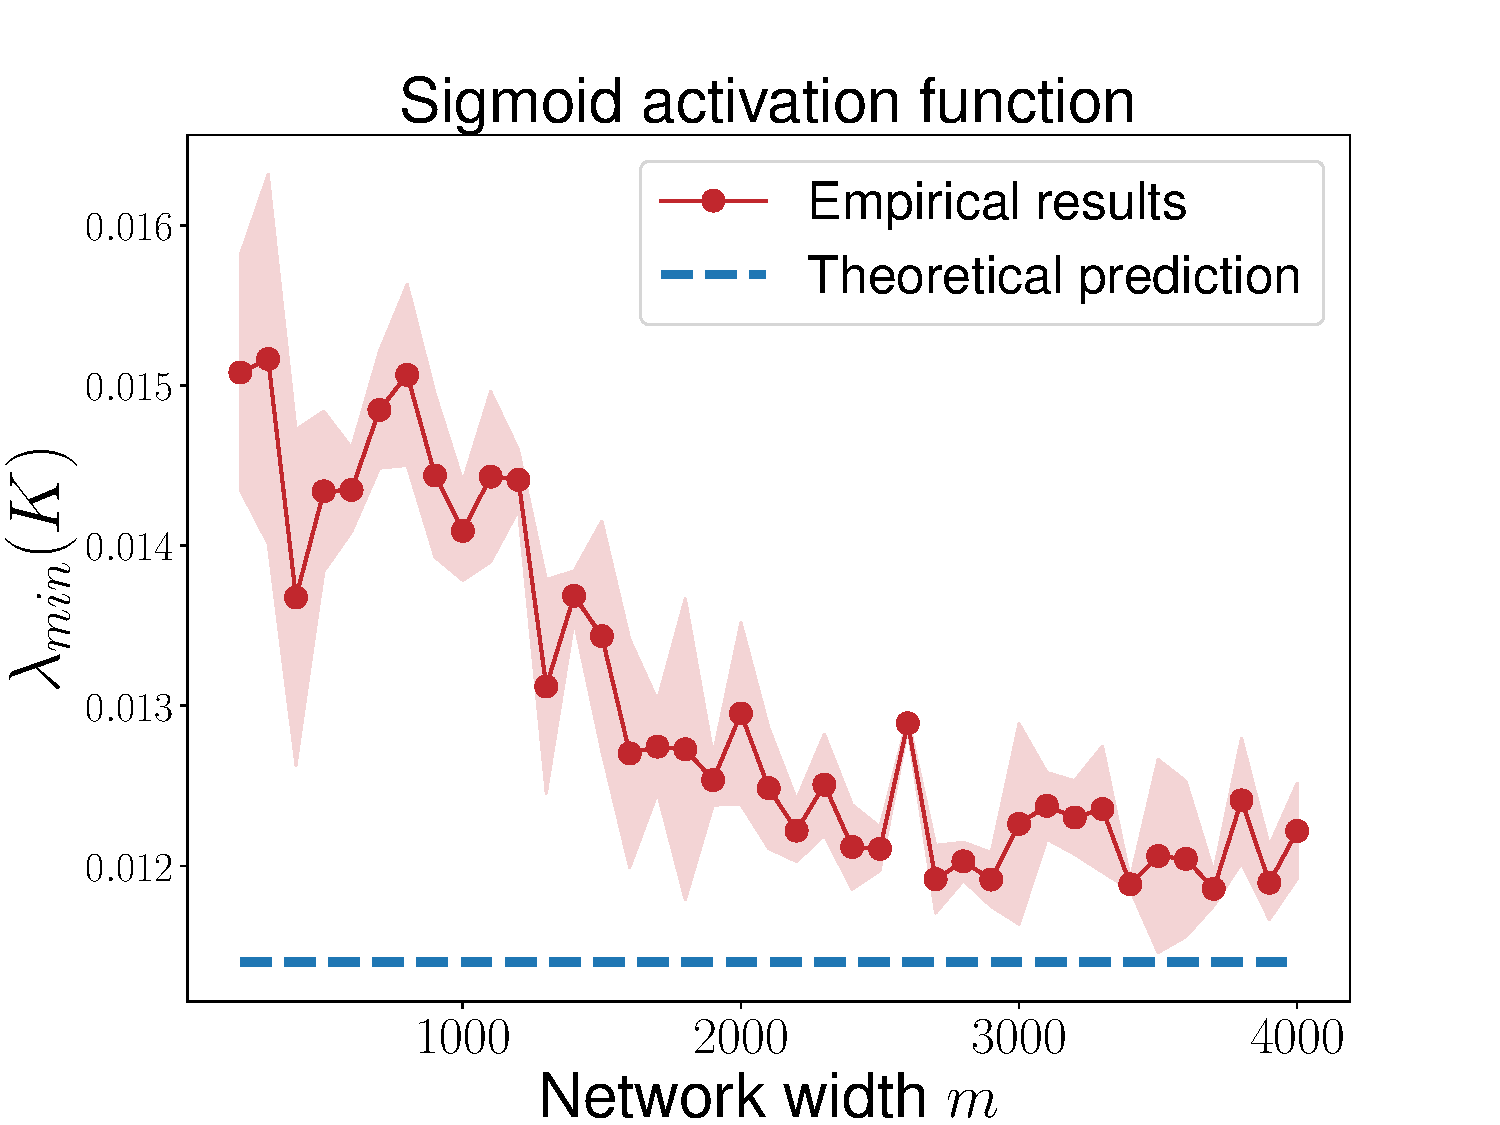
\includegraphics[width =  0.42\textwidth]{fig/min_eig_sigmoid.pdf}
 } \\
\subfigure[$\lambda_{\min}(K)$ vs.~width.]{
 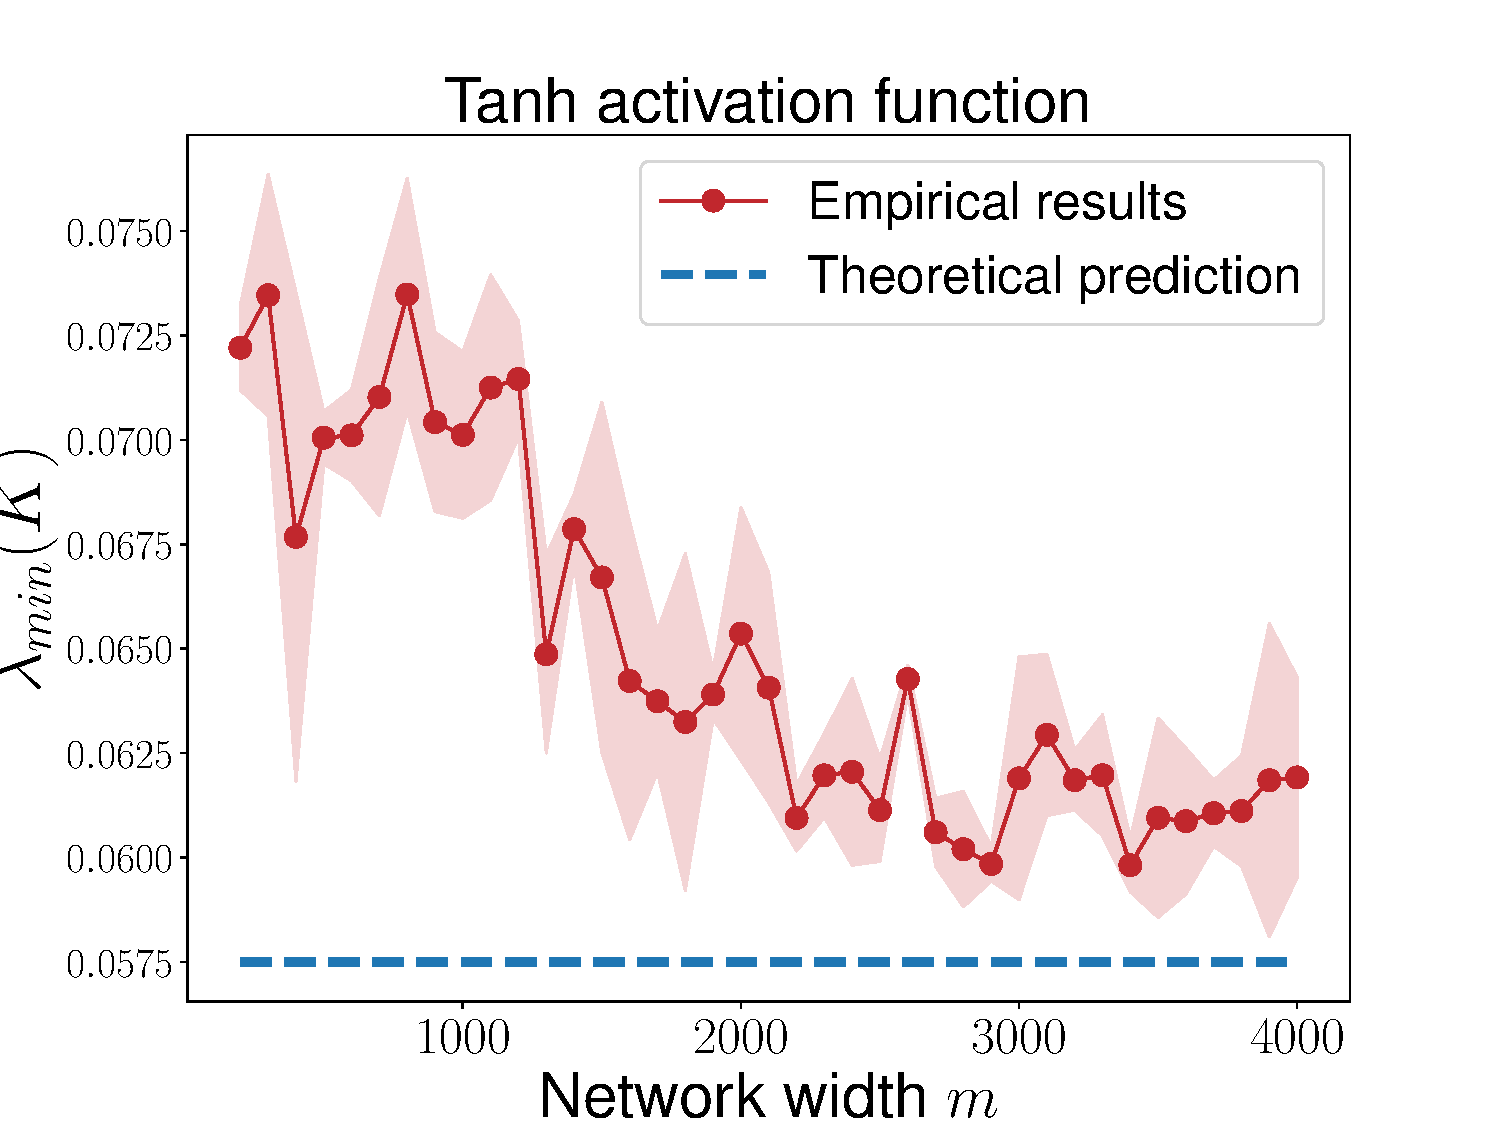
\includegraphics[width =  0.42\textwidth]{fig/min_eig_tanh.pdf}
 } 
\caption[]{Positive $\lambda_{\min}(K)$ with linear width. In the experiments, we train a 3-layer fully-connected neural network with Sigmoid/Tanh activation functions whose width has the same numerical value as the number of data points. Each curve is the average of 3 independent runs.\label{fig:min_ntk}}
\end{figure}

\section{CONCLUSIONS}
\label{sec:arXiv_conc}
In this paper,  
%we revisit deep learning optimization for feedforward models with smooth activations, and make 
we revisit the NTK analysis with smooth activations and show that effectively linear width suffices for the NTK at initialization to be positive definite. Our analysis \pcedit{makes a novel use of generalized Hermite series expansion for smooth function activation. Though standard Hermite series expansion has been used for ReLU activation functions, such analysis relied heavily on the homogeneous assumption of ReLU functions --- a property generally absent in smooth activation functions. 
\pcdelete{Our work also presents how achieving $\epsilon$-optimality can improve the width dependence on the number of training samples to be linear, thus improving the dependence over the existing literature, even when compared to works based on ReLU activations.}
Finally, our work highlights the importance of initialization variance \pcedit{in determining a trade-off between tighter Hessian bounds and larger lower bounds on the NTK condition.}}
{ Given the growing literature on optimization of neural networks based on NTK analysis, we hope our work contributes by providing a better theoretical understanding on the performance of networks whose width may beneficially scale with the number of training samples.} %\pccomment{This last sentence needs work. Maybe mention future work too.}.

%reveals a possible tradeoff based on the initialization variance, with smaller values helping the Hessian and RSC analyses and larger values helping the NTK analysis. 

%\noindent {\bf Acknowledgements.} The research was supported by NSF grants IIS 21-31335, OAC 21-30835, DBI 20-21898, and a C3.ai research award. 

%\bibliographystyle{plainurl}
\bibliographystyle{plainnat}
%\bibliographystyle{alpha}
%\bibliographystyle{apalike}
\bibliography{biblio}


%\title{NTK at Initilization: Linear Width Suffices}

%\onecolumn
%\appendix
%\maketitle



%\section{NEURAL TANGENT KERNEL AT INITIALIZATION}
%\label{app:arXiv_ntk}
%

%\theontk*

\subsection{Proof of Lemma~\ref{lemm:highproblambda}}
\label{ssec:highprobablambda}
We start with a result which explicitly shows that the output $\| \alpha^{(l)}\|_2$ is sub-Gaussian for Gaussian random weights. We recall that we are assuming $\phi(0)=0$, and note that the result can be extended to the general case straightforwardly.

\begin{lemm}
Let $A^{(l)} = [ \alpha^{(l)}(\x_i)] \in \R^{n \times m_l}$ be the outputs of layer $l$.
For $g \sim \cN(\bm{0}_{m_{l-1}},\sigma^2 \I_{m_{l-1}})$, let $\vartheta^{(l)} = \phi(\frac{1}{\sqrt{m_{l-1}}} A^{(l-1)} g ) \in \R^{n}$. Then, $\| \vartheta^{(l)}\|_2$ is a sub-Gaussian random variable with 
\begin{align*}
\| \|\vartheta^{(l)}\|_2 \|_{\psi_2} = \left\| \left\| \phi\left(\frac{1}{\sqrt{m_{l-1}}} A^{(l-1)} g \right) \right\|_2 \right\|_{\psi_2}\leq c \frac{\sqrt{2} (\sqrt{\log n} + 1)\sigma}{\sqrt{m_{l-1}}} \| A^{(l-1)} \|_F
\end{align*}
for some absolute constant $c>0$.
\label{lemm:gammasubg}
\end{lemm}
\proof First, note that since $\phi$ is 1-Lipschitz and $\phi(0) = 0$, we have $\norm{\phi( \frac{1}{\sqrt{m_{l-1}}} A^{(l-1)} g )}_2 \leq \norm{\frac{1}{\sqrt{m_{l-1}}} A^{(l-1)} g}_2$. Now, 
\begin{align*}
\P  \left( \left\| \frac{1}{\sqrt{m_{l-1}}} A^{(l-1)} g \right\|_2^2 \geq \epsilon^2 \frac{1}{m_{l-1}} \| A^{(l-1)} \|_F^2 \right)
 &= \P \left( \frac{1}{m_{l-1}} \sum_{i=1}^n \langle \alpha_i^{(l-1)}, g \rangle^2 \geq \epsilon^2 \frac{1}{m_{l-1}} \sum_{i=1}^n \| \alpha_i^{(l-1)} \|_2^2 \right)\\
& \leq \sum_{i=1}^n \P \left( \frac{1}{m_{l-1}} \langle \alpha_i^{(l-1)}, g \rangle^2 \geq \epsilon^2 \frac{1}{m_{l-1}} \| \alpha_i^{(l-1)} \|_2^2 \right) \\
& = \sum_{i=1}^n \P \left( |\langle \alpha_i^{(l-1)}, g \rangle| \geq \epsilon \| \alpha_i^{(l-1)} \|_2 \right)\\
& \leq 2n \exp\left( - \frac{\epsilon^2}{2\sigma^2} \right)~.
\end{align*}
In other words, with $\tilde{\epsilon} = \frac{\epsilon}{\sqrt{m_{l-1}}} \| A^{(l-1)} \|_F$, for all $\tilde{\epsilon} > 0$ we have 
\begin{align*}
\P \left( \left\| \frac{1}{\sqrt{m_{l-1}}} A^{(l-1)} g \right\|_2 \geq \tilde{\epsilon} \right) \leq 2n \exp\left( - \frac{m_{l-1} \tilde{\epsilon}^2}{2\sigma^2 \| A^{(l-1)} \|^2_F } \right) ~.
\end{align*}
Now, with $\tilde{\epsilon} = \frac{\sigma \sqrt{2 \log n} }{\sqrt{m_{l-1}}} \| A^{(l-1)} \|_F + \epsilon $, for all $\epsilon > 0$ we have
\begin{align*}
\P \left( \left\| \frac{1}{\sqrt{m_{l-1}}} A^{(l-1)} g \right\|_2  \geq  \frac{\sigma \sqrt{2 \log n}}{\sqrt{m_{l-1}}} \| A^{(l-1)} \|_F + \epsilon  \right) & \leq 2n \exp \left( - \log n \right)  \exp\left( - \frac{m_{l-1} \epsilon^2}{2\sigma^2 \| A^{(l-1)} \|^2_F } \right) \\
\Rightarrow ~~~\P \left( \left\| \phi\left( \frac{1}{\sqrt{m_{l-1}}} A^{(l-1)} g \right) \right\|_2  \geq  \frac{\sigma \sqrt{2 \log n }}{\sqrt{m_{l-1}}} \| A^{(l-1)} \|_F + \epsilon  \right) & \leq 2 \exp\left( - \frac{m_{l-1} \epsilon^2}{2\sigma^2 \| A^{(l-1)} \|^2_F } \right)~.
\end{align*}
Then, from Proposition~\ref{prop:subgsum}, it follows that $\| \phi( \frac{1}{\sqrt{m_{l-1}}} A^{(l-1)} g ) \|_2$ is sub-Gaussian with 
\begin{align*}
\left\| \left\| \phi\left( \frac{1}{\sqrt{m_{l-1}}} A^{(l-1)} g \right) \right\|_2 \right\|_{\psi_2} \leq c \frac{\sqrt{2} (\sqrt{\log n} + 1)\sigma}{\sqrt{m_{l-1}}} \| A^{(l-1)} \|_F~,
\end{align*}
for some absolute constant $c$. This completes the proof. \qed 

\begin{prop}
Let $a_1, a_2 > 0$. If a non-negative random variable $Z$ satisfies $\P( Z \geq a_1 + \epsilon) \leq 2 \exp(-\epsilon^2/a_2^2)$, then $\| Z \|_{\psi_2} \leq c(a_1 + a_2)$, where $c$ is an absolute constant.
\label{prop:subgsum}
\end{prop}
\proof Note that $Z-a_1 = [Z-a_1]_- + [Z-a_1]_+$. Since $Z$ is non-negative, $|[Z-a_1]_-| \leq a_1$ implying $\|[Z-a_1]_-\|_{\psi_2} \leq c_1 a_1$, where $c_1$ is an absolute constant. Further, by definition, $[Z-a_1]_+$ is sub-Gaussian with $\| [Z-a_1]_+ \|_{\psi_2} \leq c_2 a_2$, where $c_2$ is an absolute constant. Now, by triangle inequality
\begin{align*}
\| Z \|_{\psi_2} & = \| a_1 + [Z-a_1]_- + [Z - a_1]_+ \|_{\psi_2} \\
& \leq a_1 + \|[Z-a_1]_-\|_{\psi_2} + \| [Z-a_1]_+ \|_{\psi_2} \leq a_1 + c_1 a_1 + c_2 a_2\\
& \leq c(a_1+a_2)~,
\end{align*}
where $c = \max(1+c_1, c_2)$. That competes the proof. \qed

% \abcomment{update the analysis -- can be done more directly, using Hoeffding(?)} Let $U = \left\{u_i = \frac{\alpha_i}{\| \alpha_i\|_2}, i \in [n]\right\}$ so that $u_i \in \R^{m_l}, i \in [n]$. Then, from Lemma~\ref{lem:newaux1}, with probability at least $(1-2\exp(-\tau^2/(2\sigma_0^2)))$, we have 
% \begin{align*}
% \frac{1}{\| \alpha_i^{(l-1)} \|_2} \| W_0^{(l)} \alpha_i^{(l)} \|_2  =  \| W_0^{(l)} u_i \|_2 \leq \sigma_0(\sqrt{m} + \sqrt{\log n}) + \tau~,
% \end{align*}
% since $W_0^{(l)} \in \R^{m_{l} \times m_{l-1}}$ has entries $w_{0,ij}^{(l)} \sim \cN(0,\sigma_0^2)$.
% % Then, from the proof on Lemma~\ref{lemm:outl2} and Assumption~\ref{asmp:ginit}, with probability at least $(1-2\exp(-\tau^2/(2\sigma_0^2)))$, we have 
% % \begin{align*}
% % ~\frac{1}{\| \alpha_i^{(l-1)} \|_2} \| W^{(l)} \alpha_i^{(l-1)} \|_2  \leq \sqrt{m}\left( \sigma_1 + \frac{\rho}{\sqrt{m}} \right) + \tau = \sqrt{m} \gamma + \tau~.
% % \end{align*}
% Since $\phi(0)=0$, with probability at least $(1-2\exp(-\tau^2/(2\sigma_0^2)))$, we have 
% \begin{align*}
% \| \alpha_i^{(l)} \|_2 & \leq ~\left\| \frac{1}{\sqrt{m_{l-1}}} W_0^{l} \alpha_i^{(l-1)} \right\|_2 
%  \leq \left(\gamma + \frac{\tau  }{\sqrt{m}} \right) \| \alpha_i^{(l-1)} \|_2~.
% \end{align*}
% Then, with probability at least $(1-2\exp(-\tau^2/(2\sigma_0^2)))$, we have 
% \begin{align*}
% \| \Gamma^{(l)} \|^2_2 & = \sum_{i=1}^n \left\| \phi\left( \frac{1}{\sqrt{m}} \langle \alpha_i^{(l-1)}, g \rangle\right) \right\|^2_2 \leq  \left(\gamma + \frac{\tau  }{\sqrt{m}} \right)^2 \| A^{(l-1)} \|_F^2~\\
% \Rightarrow \qquad \| \Gamma^{(l)} \|_F & \leq \gamma \| A^{(l-1)} \|_F + \frac{ \tau \| A^{(l-1)} \|_F}{\sqrt{m}}~.
% \end{align*}
% Then, with $t = \frac{ \| A^{(l-1)} \|_F}{\sqrt{m}} \tau$, we have with probability at least $(1 - 2\exp(-\frac{m t^2}{2 \sigma_0^2 \| A^{(l-1)} \|_F^2})$, we have 
% \begin{align*}
% \| \Gamma^{(l)} \|_F \leq \gamma \| A^{(l-1)} \|_F + t~,
% \end{align*}
% Then, from \abedit{Proposition ??} it follows that $\| \Gamma^{(l)} \|_F$ is a sub-Gaussian random variable with $\| \Gamma^{(l)} \|_{\psi_2} \leq \gamma \| A^{(l-1)}\|_F + \frac{\sigma_0 \| A^{(l-1)} |_F}{\sqrt{m}} \leq \left( \gamma + \frac{\sigma_1}{\sqrt{m}} \right) \| A^{(l-1)}\|_F$, since $\sigma_0 \leq \sigma_1$. That completes the proof. \qed 

We are now ready to prove Lemma~\ref{lemm:highproblambda}.
%
%\highproblambda*

\proof[Proof of Lemma~\ref{lemm:highproblambda}] Let $\vartheta^{(l)} = \phi(\frac{1}{\sqrt{m_{l-1}}} A^{(l-1)} g) \in \R^{n}$. If $m_l < n$, then $\lambda_{\min}(A^{(l)} (A^{(l)})^\top) = 0$. So, we assume $m_l \geq n$.
%
Let $w_j \in \R^{m_{l-1}}$ denote the $j$-th row of $W_0^{(l)}$.
For a given $t>0$, let $\hat{A}^{(l)} \in \R^{n \times m_l}$ so that $\hat{A}_{:,j}^{(l)} = \phi( \frac{1}{\sqrt{m_l}} A^{(l-1)} w_j^\top ) \1_{[\| \phi(\frac{1}{\sqrt{m_l}} A^{(l-1)} w_j^\top \|_2 \leq t]}\in\R^{m_{l-1}}$ and $\hat{\vartheta}^{(l)} = \phi( \frac{1}{\sqrt{m_l}} A^{(l-1)} g ) \1_{[\| \phi(\frac{1}{\sqrt{m_l}} A^{(l-1)} g \|_2 \leq t]} \in \R^n$. Then, we have 
%\lzcomment{I did not find the proof of $\lambda_{\max}$?}
\begin{align*}
(i)\;\; &
\lambda_{\min}( A^{(l)} ( A^{(l)})^\top ) \geq \lambda_{\min}( \hat{A}^{(l)} ( \hat{A}^{(l)})^\top )  ~,\\
(ii)\;\;&\lambda_{\max}( \hat{A}_{:,j}^{(l)} ( \hat{A}_{:,j}^{(l)})^\top ) \leq t^2~,
\end{align*}
where (i) follows immediately by definition of $\hat{A}^{(l)}$ and (ii) follows since for any unit vector $v \in \R^n$, 
%\begin{align*}
$v^\top \hat{A}_{:,j}^{(l)} ( \hat{A}_{:,j}^{(l)})^\top v = \langle v, \hat{A}_{:,j}^{(l)} \rangle^2 \leq \| \hat{A}_{:,j}^{(l)} \|_2^2 \leq t^2$.
%\end{align*}

From Lemma~\ref{lemm:gammasubg}, we know that $\| \| \vartheta^{(l)} \|_2 \|_{\psi_2} \leq c_1  \frac{\sqrt{2}(\sqrt{\log n}+1)\sigma}{\sqrt{m}} \| A^{(l-1)} \|_F$.  Recall that for any subGaussian random variable $Z$, $\P(Z \geq t) \leq \exp(1-c t^2/\| Z \|_{\psi_2}^2)$ for some absolute constant $c$. For our analysis with $\| \vartheta^{(l)} \|_2$, for a suitable constant $a > 0$ we will use 
\begin{align}
    t = \frac{  \sqrt{2} (\sqrt{\log n}+1) \sigma \| A^{(l-1)} \|_F}{\sqrt{cm_{l-1}}} \sqrt{ \max \left(1 , \log \frac{2a (\sqrt{\log n} + 1)^2 \sigma^2 \| A^{(l-1)} \|_F^2}{ c \lambda_l m_{l-1}} \right) }~.
\label{eq:thres}
\end{align}

Let
\begin{align*}
\hspace*{-10mm}
G_l & := \E_{g \sim \cN(\bm{0}_{m_{l-1}},\sigma^2 \I_{m_{l-1}})}\left[ \vartheta^{(l)} (\vartheta^{(l)})^\top \right] = \E_{g \sim \cN(\bm{0}_{m_{l-1}},\sigma^2 \I_{m_{l-1}})}\left[ \phi\left( \frac{1}{\sqrt{m_{l-1}}} A^{(l-1)} g \right) \phi\left( \frac{1}{\sqrt{m_{l-1}}} A^{(l-1)} g \right)^\top \right] ~, \\
\hat{G}_l & := \E_{g \sim \cN(\bm{0}_{m_{l-1}},\sigma^2 \I_{m_{l-1}})}\left[ \hat{\vartheta}^{(l)} (\hat{\vartheta}^{(l)})^\top \right] \\
& ~~= \E_{g \sim \cN(\bm{0}_{m_{l-1}},\sigma^2 \I_{m_{l-1}})}\left[ \phi\left( \frac{1}{\sqrt{m_{l-1}}} A^{(l-1)} g\right) \phi \left( \frac{1}{\sqrt{m_{l-1}}} A^{(l-1)} g \right)^\top \1_{[\| \phi ( \frac{1}{\sqrt{m_{l-1}}} A^{(l-1)} g) \|_2 \leq t]} \right] ~. 
\end{align*}
Note that $\lambda_l = \lambda_{\min}(G_l)$.

By Matrix Chernoff bound, for any $\epsilon \in [0,1)$, we have
\begin{align*}
\P\left( \lambda_{\min}( \hat{A}^{(l)} ( \hat{A}^{(l)})^\top ) \leq (1-\epsilon) \lambda_{\min}( \E_{W_0^{(l)}}[ \hat{A}^{(l)} ( \hat{A}^{(l)})^\top ]) \right) \leq n \left(\frac{e^{-\epsilon}}{(1-\epsilon)^{1-\epsilon}} \right)^{\lambda_{\min}\left(\E_{W_0^{(l)}}[\hat{A}^{(l)} ( \hat{A}^{(l)})^\top ]\right)/t^2}~.
\end{align*}
For $\epsilon=1/2$, with $c_3 = \frac{1}{2}(1 - \log 2)$, we have 
\begin{align*}
\P\left( \lambda_{\min}( \hat{A}^{(l)} ( \hat{A}^{(l)})^\top ) \leq \frac{m_l}{2} \lambda_{\min}(\hat{G}_l) \right) \leq \exp\left( - \frac{c_3 m_l}{t^2} \lambda_{\min}(\hat{G}) + \log n \right)~,
\end{align*}
where we used the fact that $\E_{W_0^{(l)}}[\hat{A}^{(l)}(\hat{A}^{(l)})^\top]=m_l\E_{g \sim \cN(\bm{0}_{m_{l-1}},\sigma^2 \I_{m_{l-1}})}[\hat{\vartheta}^{(l)}(\hat{\vartheta}^{(l)})^\top]=m_l\hat{G}_l$. 

With $m_l \geq \frac{t^2}{c_3 \lambda_{\min}(\hat{G}_l)} \log \frac{n}{\bar{\delta}}$, with probability at least $(1-\bar{\delta})$ we have 
\begin{align}
\label{eq:lowerbound_hat_A_l}
\lambda_{\min}( \hat{A}^{(l)} ( \hat{A}^{(l)})^\top ) \geq \frac{m_l}{2} \lambda_{\min}(\hat{G}_l) ~.
\end{align}
Now, note that
\begin{align*}
\hspace*{-25mm}
\| \hat{G}_l - G_l \|_2 & \leq 
 \E_{g \sim \cN(\bm{0}_{m_{l-1}},\sigma^2 \I_{m_{l-1}})} \left\|  \phi\left( \frac{1}{\sqrt{m_{l-1}}} A^{(l-1)} g\right) \phi \left( \frac{1}{\sqrt{m_{l-1}}} A^{(l-1)} g \right)^\top \1_{[\| \phi ( \frac{1}{\sqrt{m_{l-1}}} A^{(l-1)} g) \|_2 \leq t]} \right. \\
 &  \left. \phantom{\E   \phi\left( \frac{1}{\sqrt{m_{l-1}}} A^{(l-1)} g\right) \phi \left( \frac{1}{\sqrt{m_{l-1}}} A^{(l-1)} g \right)^\top } 
 -  \phi\left( \frac{1}{\sqrt{m_{l-1}}} A^{(l-1)} g \right) \phi\left( \frac{1}{\sqrt{m_{l-1}}} A^{(l-1)} g \right)^\top \right\|_2 \\
& = \E_{g \sim \cN(\bm{0}_{m_{l-1}},\sigma^2 \I_{m_{l-1}})}\left[ \left\| \phi \left( \frac{1}{\sqrt{m_{l-1}}} A^{(l-1)} g \right) \right\|_2^2 \1_{[\| \phi ( \frac{1}{\sqrt{m_{l-1}}} A^{(l-1)} g) \|_2 > t]} \right]    \\
& \overset{(a)}{=} \int_{s=0}^{\infty} \P\left( \left\| \phi \left( \frac{1}{\sqrt{m_{l-1}}} A^{(l-1)} g \right) \right\|_2 \1_{[\| \phi ( \frac{1}{\sqrt{m_{l-1}}} A^{(l-1)} g) \|_2 > t]} > \sqrt{s} \right) ds \\
& = \int_{s=0}^{\infty} \P\left( \left\| \phi \left( \frac{1}{\sqrt{m_{l-1}}} A^{(l-1)} g \right) \right\|_2 > t \right) \P\left( \left\| \phi \left( \frac{1}{\sqrt{m_{l-1}}} A^{(l-1)} g \right) \right\|_2 > \sqrt{s} \right) ds \\
& \overset{(b)}{\leq}\exp(2) \exp\left( -c \frac{m_{l-1} t^2 }{2(\sqrt{\log n} +1)^2 \sigma^2 \| A^{(l-1)} \|_F^2} \right) \int_{s=0}^{\infty} \exp\left( -c \frac{m_{l-1} s }{2(\sqrt{\log n} +1)^2 \sigma^2 \| A^{(l-1)} \|_F^2} \right) ds \\
& \overset{(c)}{=} \exp(2) \exp\left( -  \max\left(1 , \log \frac{2a (\sqrt{\log n}  + 1)^2 \sigma^2 \| A^{(l-1)} \|_F^2}{c \lambda_l m_{l-1}} \right)  \right) \frac{2(\sqrt{\log n} +1)^2 \sigma^2 \|A^{(l-1)}\|_F^2}{cm_{l-1}} ~,
\end{align*}
where (a) follows since for any non-negative random variable $Z$,  $\E[Z] = \int_0^{\infty} \P(Z \geq s) ds$, (b) follows from Lemma~\ref{lemm:gammasubg}, and (c) follows from our choice of  $t$ in \eqref{eq:thres} and since for $b > 0$, $\int_0^\infty \exp(-s/b) ds = b$. To simplify further, we consider the following two exhaustive cases:

{\bf Case 1.} Assume
\begin{align*}
\frac{2a(\sqrt{\log n}  + 1)^2 \sigma^2 \| A^{(l-1)} \|_F^2}{c \lambda_l m_{l-1}} \leq \exp(1) \quad \Rightarrow \quad \frac{2 (\sqrt{\log n}  + 1)^2 \sigma^2 \| A^{(l-1)} \|_F^2}{c m_{l-1} }  \leq \frac{\lambda_l}{a} \exp(1)~. 
\end{align*}
Then,
\begin{align*}
\| \hat{G}_l - G_l \|_2 & \leq \exp(2) \exp(-1) \frac{2(\sqrt{\log n} +1)^2 \sigma^2 \|A^{(l-1)}\|_F^2}{cm_{l-1}}  \leq \exp(2) \exp(-1) \exp(1) \frac{\lambda_l}{a} = \frac{\exp(2)}{a} \lambda_l \overset{(a)}{\leq} \frac{\lambda_l}{2}~,
\end{align*}
where (a) follows if $a \geq 2 \exp(2)$.

{\bf Case 2.} On the other hand, assume
\begin{align*}
\frac{2a(\sqrt{\log n}  + 1)^2 \sigma^2 \| A^{(l-1)} \|_F^2}{c m_{l-1} \lambda_l} \geq \exp(1) ~. 
\end{align*}
Then,
\begin{align*}
\| \hat{G}_l - G_l \|_2 & \leq \exp(2) \frac{c \lambda_l m_{l-1}}{2a (\sqrt{\log n}+1)^2 \sigma^2 \| A^{(l-1)} \|_F^2}  \frac{2(\sqrt{\log n} +1)^2 \sigma^2 \|A^{(l-1)}\|_F^2}{cm_{l-1}} = \frac{\exp(2)}{a} \lambda_l \overset{(a)}{\leq} \frac{\lambda_l}{2}~,
\end{align*}
where (a) follows if $a \geq 2 \exp(2)$. Thus, choosing $a = 15$ in \eqref{eq:thres} ensures $\| \hat{G}_l - G_l \|_2 \leq \frac{\lambda_l}{2}$. As a result, 
\begin{equation}
    \label{eq:lowerbound_hat_A_to_A_l}
\lambda_{\min}(\hat{G}_l) \geq \lambda_{\min}(G_l) - \|\hat{G}_l - G_l \|_2 \geq \lambda_l/2.
\end{equation}
Then, for $m_l \geq \frac{2t^2}{c_3 \lambda_l} \log \frac{n}{\bar{\delta}}$, with probability at least $(1-\bar{\delta})$ we have 
\begin{align*}
\lambda_{\min}(A^{(l)} (A^{(l)})^\top ) & \geq \lambda_{\min}(\hat{A}^{(l)} (\hat{A}^{(l)})^\top ) \overset{(a)}{\geq} \frac{m_l}{2} \lambda_{\min}(\hat{G}) \overset{(b)}{\geq} \frac{m_l}{4} \lambda_l~.
\end{align*}
where (a) follows from~\eqref{eq:lowerbound_hat_A_l} and (b) from~\eqref{eq:lowerbound_hat_A_to_A_l}. Finally, note that we have used $m_l \geq n$ and $m_l \geq \frac{t^2}{c_3 \lambda_{\min}(\hat{G})} \log \frac{n}{\bar{\delta}}$ in the above analysis. Then, with $v = \frac{2 (\sqrt{ \log n} +1)^2 \sigma^2 \| A^{(l-1)} \|_F^2}{c_3 \lambda_l m_{l-1} }$, the choice of $t$ in \eqref{eq:thres}, and $a=15$, and noting that $\lambda_{\min}(\hat{G}) \geq \lambda_l/2$, the analysis holds if we have
\begin{align*}
m_l & \geq \max \left( n,c_2 v \max(1, \log (15 v)) \log \frac{n}{\bar{\delta}} \right)~.
\end{align*}
for some constant $c_2 > 0$. Choosing $\bar{\delta} = \frac{\delta}{L}$ completes the proof. \qed 


\subsection{Proof of Lemma~\ref{lemm:alphainit1}}
\label{ssec:alphainit}



% We present two versions of a result which establishes $\| \alpha^l(\x)\|_2^2 = \Theta(m)$. For the first, we assume the Gaussian variance is $\frac{\sigma_0^2}{c_{\phi,\sigma_0}}$ where $c_{\phi,\sigma_0} := \E_{z \sim \cN(0,\sigma_0^2)}[\phi^2(z)]$. For the second form, we keep the Gaussian variance as $\sigma_0^2$ but used a scaled activation function: $\bar{\phi}(a) = \frac{1}{\sqrt{c_{\phi,\sigma_0}}} \phi(a)$. Both versions yield effectively the same result and are equivalent.  
% \begin{remark}
% \abcomment{update ... their analysis was incorrect} Such scaling has appeared in earlier work with smooth activation functions [Du et al.].
% \end{remark}

% \alphainit*

% \proof We do the proof by induction. For $l=0$, $\| \alpha^{(0)}(\x) \|_2^2 = \| x \|_2^2 =  c_{\phi,\sigma_0} d$.  For $l=0$ and $m_0 = d$, so the result is satisfied at $l=0$ almost surely.

% Assume that the result holds for a certain $l$, so that
% \begin{align}
% c_{\phi,\sigma_0} \left(1 -  \frac{h_C(l)}{2h_C(L)}\right) m_l  \leq \| \alpha^l(\x) \|_2^2 \leq c_{\phi,\sigma_0} \left(1 +  \frac{h_C(l)}{2h_C(L)}\right) m_l \nonumber  \\
% \Rightarrow \quad - \frac{h_C(l)}{2h_C(L)}  \leq \frac{\| \alpha^l(\x) \|_2^2}{c_{\phi,\sigma_0} m_l} - 1 \leq  \frac{h_C(l)}{2h_C(L)} ~.
% \label{eq:rip1}
% \end{align}
% We condition on $\{ W_0^{(l')}, l' \in [l] \}$, and focus on layer $\alpha^{(l+1)}$ with random weights $W_0^{(l+1)} = [w_{1,:}; \cdots;w_{m_{l+1},:}] \in \R^{m_{l+1} \times m_l}$. Note that $\|\alpha^{(l+1)}(\x) \|_2^2 = \sum_{j=1}^{m_{l+1}} (\alpha^{(l+1)}_j(\x))^2$.  Since $\phi$ is 1-Lipschitz and $\phi(0)=0$, $|\phi(a)| \leq |a|$, we have
% \begin{align}
% \E_{W_0^{(l+1)}}\| \alpha^{(l+1)}(\x) \|_2^2 & = \sum_{j=1}^{m_{l+1}} \E_{w_{j,:}} [(\alpha^{(l+1)}_j(\x))^2] = m_{l+1} \E_{g \sim \cN\left(0,\frac{\sigma_0^2}{c_{\phi,\sigma_0}} \I\right)}\left[ \phi^2\left(\frac{1}{\sqrt{m_l}}\langle g, \alpha^{(l)}(\x) \rangle \right) \right]~\nonumber \\
% & = m_{l+1} \E_{g \sim \cN\left(0,\frac{\sigma_0^2}{c_{\phi,\sigma_0}} \I\right)}\left[ \phi^2\left(\frac{\| \alpha^{(l)}(\x)\|_2}{\sqrt{m_l}} \left\langle g, \frac{\alpha^{(l)}(\x)}{\| \alpha^{(l)}(\x)\|_2} \right\rangle \right) \right] \nonumber \\
% & = m_{l+1}  \E_{z \sim \cN\left(0,\frac{\sigma_0^2}{c_{\phi,\sigma_0}}\right)}\left[ \phi^2\left(\frac{\| \alpha^{(l)}(\x)\|_2}{\sqrt{m_l}} z \right) \right] \\
% & = m_{l+1}  \E_{z \sim \cN(0,\sigma_0^2)}\left[ \phi^2\left(\frac{\| \alpha^{(l)}(\x)\|_2}{\sqrt{c_{\phi,\sigma_0}m_l}} z \right) \right]
% \label{eq:rip2}
% \end{align}
% From Proposition~\ref{prop:gauss2} with $\beta = \frac{\| \alpha^{(l)}(\x)\|_2}{\sqrt{c_{\phi,\sigma_0 m_l}}}$, we have 
% \begin{align}
% c_{\phi,\sigma_0} - \sigma_0^2 \left| \frac{\| \alpha^l(\x) \|_2^2}{c_{\phi,\sigma_0} m_l} - 1 \right| & \leq \E_{z \sim \cN(0,\sigma_0^2)}\left[ \phi^2\left(\frac{\| \alpha^{(l)}(\x)\|_2}{\sqrt{c_{\phi,\sigma_0}m_l}} z \right) \right] 
%     \leq c_{\phi,\sigma_0} + \sigma_0^2 \left| \frac{\| \alpha^l(\x) \|_2^2}{c_{\phi,\sigma_0} m_l} - 1 \right| \nonumber \\
% \overset{(a)}{\Rightarrow} \quad c_{\phi,\sigma_0}\left( 1 - \frac{c_0 h_C(l)}{2h_C(L)} \right) & \leq \E_{z \sim \cN(0,\sigma_0^2)}\left[ \phi^2\left(\frac{\| \alpha^{(l)}(\x)\|_2}{\sqrt{c_{\phi,\sigma_0} m_l}} z \right) \right] 
%   \leq c_{\phi,\sigma_0}\left( 1 + \frac{c_0 h_C(l)}{2h_C(L)} \right)~,  
% %\Rightarrow \quad c_{\phi,\sigma_0}\left( 1 - \frac{h_C(l+1)}{2h_C(L)} \right) & \leq \E_{z \sim \cN(0,\sigma_0^2)}\left[ \phi^2\left(\frac{\| \alpha^{(l)}(\x)\|_2}{\sqrt{m_l}} z \right) \right]   \leq c_{\phi,\sigma_0}\left( 1 + \frac{h_C(l+1)}{2h_C(L)} \right)~,
%  \label{eq:rip3}
% \end{align}
% where (a) follows from \eqref{eq:rip1}. 
% %and (b) follows by the definition of $h_C(l)$.

% Combining \eqref{eq:rip2} and \eqref{eq:rip3}, we have 
% \begin{align}
% c_{\phi,\sigma_0} \left(1 -  \frac{c_0 h_C(l)}{2h_C(L)}\right) m_{l+1}  \leq \E_{W_0^{(l+1)}}\| \alpha^{(l+1)}(\x) \|_2^2 \leq c_{\phi,\sigma_0} \left(1 +  \frac{c_0 h_C(l)}{2h_C(L)}\right) m_{l+1}~.
% \label{eq:rip4}
% \end{align}

% Let $\kappa:= \| (\alpha_j^{(l+1)}(\x))^2 \|_{\psi_1}$. Then, from Lemma~\ref{lemm:gammasubg} and \eqref{eq:rip1}, we have
% $\kappa  = \| (\alpha_j^{(l+1)}(\x)) \|^2_{\psi_2} \leq \frac{4 \sigma^2}{m_l} \| \alpha^{(l)} \|_2^2 \leq 6 c_{\phi,\sigma_0} \sigma^2 = \tilde{O}(1)$. Conditioned on $\{ W_0^{(l')}, l' \in [l] \}$, since $\alpha_j^{(l+1)}(\x), j \in [m_{l+1}]$ are independent, from Bernstein's inequality we have 
% \begin{align*}
% \P\left( \left| \sum_{j=1}^{m_{l+1}} (\alpha_j^{(l+1)}(\x))^2 - \E_{W_0^{(l+1)}}\| \alpha^{(l+1)}(\x) \|_2^2  \right| \geq t \right) \leq 2 \exp\left[-c \min\left(\frac{t^2}{m_{l+1} \kappa^2} , \frac{t}{\kappa} \right) \right]
% \end{align*}
% Choosing $t = \frac{c_{\phi,\sigma_0}}{2h_C(L)} \frac{\kappa}{\min(c,\sqrt{c})} (m_{l+1})^{3/4} \log m_{l+1} \leq \frac{c_{\phi,\sigma_0}}{2h_C(L)} m_{l+1}$, we have 
% \begin{align*}
% \E_{W_0^{(l+1)}}\| \alpha^{(l+1)}(\x) \|_2^2 - \frac{c_{\phi,\sigma_0}}{2h_C(L)} m_{l+1}  & ~\leq~  \| \alpha^{(l+1)}(\x) \|_2^2  ~\leq~  E_{W_0^{(l+1)}}\| \alpha^{(l+1)}(\x) \|_2^2 + \frac{c_{\phi,\sigma_0}}{2h_C(L)} m_{l+1} \\
% \overset{(a)}{\Rightarrow} \quad  c_{\phi,\sigma_0} \left( 1 - \frac{1 + c_0 h_C(l)}{2h_C(L)} \right) m_{l+1} & ~\leq ~  \| \alpha^{(l+1)}(\x) \|_2^2  ~ \leq ~  c_{\phi,\sigma_0} \left( 1 - \frac{1 + c_0 h_C(l)}{2h_C(L)} \right) m_{l+1} \\
% \overset{(b)}{\Rightarrow} \quad c_{\phi,\sigma_0} \left( 1 - \frac{h_C(l+1)}{2h_C(L)} \right) m_{l+1} & ~\leq ~  \| \alpha^{(l+1)}(\x) \|_2^2  ~ \leq ~  c_{\phi,\sigma_0} \left( 1 - \frac{h_C(l+1)}{2h_C(L)} \right) m_{l+1}~,
% \end{align*}
% where (a) follows from \eqref{eq:rip4} and (b) follows since $h_C(l+1) = 1 + c_0 h_C(l)$, with probability at least 
% \begin{align*}
% 1 - 2 \exp\left[ - \min \left( \frac{c^2_{\phi,\sigma_0} \sqrt{m_{l+1}}}{8 h_C(L)^2}, \frac{c_{\phi,\sigma_0} \sqrt{m_{l+1}}}{4 h_C(L)}  \right) 2\log m_{l+1}\right] \leq 1 - \frac{2}{m_l}~.
% \end{align*}
% Applying union bound over all layers completes the proof. \qed 

% \abedit{Let $a_0 = c_0^2$. Recall that $L \leq \log n$, we have $h_C(L) = \frac{c_0^L-1}{c_0 - 1} \leq L c_0^L$, so that $h_C^2(L) \leq L^2 (a_0)^L \leq (\log n)^2 a_0^L \leq (\log n)^2 n^{\log a_0}$. Then, it suffices to have $m_{l+1} = \tilde{\Omega}(n^{\log a_0})$ where $a_0 = c_0^2 = \frac{\sigma_0^4}{c_{\phi,\sigma}^2}$. For $\phi(a)=a$, $c_0=a_0=1$, so from this analysis, $\tilde{\Omega}(1)$ width suffices (but linear may break due to other reasons). For ReLU, $c_0 = 2$, so $a_0=4$, and $\tilde{\Omega}(n^{1.39})$ width suffices, for this part of the analysis. For GeLU, $c_0$ will be a bit smaller, so mildly larger width will be needed}
%
% \abcomment{write the above formally ... we have the result!}

%\alphainit*

\proof[Proof of Lemma~\ref{lemm:alphainit1}] We do the proof by induction. Let $\x \in \{\x_i, i \in [n]\}$. For $l=0$, $\| \alpha^{(0)}(\x_i) \|_2^2 = \| x_i \|_2^2 =  c_{\phi,\sigma_0} d$.  For $l=0$ and $m_0 = d$, so the result is satisfied at $l=0$ almost surely.

Assume that the result holds for a certain $l$, so that for any $i \in [n]$
\begin{align}
c_{\phi,\sigma_0} \left(1 -  \frac{h_C(l)}{2h_C(L)}\right) m_l   \leq \min_{i \in [n]} \| \alpha^l(\x) \|_2^2 & \leq \max_{i \in [n]} \| \alpha^{(l)}(\x) \|_2^2 \leq c_{\phi,\sigma_0} \left(1 +  \frac{h_C(l)}{2h_C(L)}\right) m_l \nonumber  \\
\Rightarrow \quad \max_{i \in [n]} \left| \frac{\| \alpha^{(l)}(\x) \|_2^2}{c_{\phi,\sigma_0} m_l} - 1 \right| & \leq  \frac{h_C(l)}{2h_C(L)} ~.
\label{eq:rip1}
\end{align}
We condition on $\{ W_0^{(l')}, l' \in [l] \}$, and focus on layer $\alpha^{(l+1)}$ with random weights $W_0^{(l+1)} = [w_{1,:}; \cdots;w_{m_{l+1},:}] \in \R^{m_{l+1} \times m_l}$. Note that $\|\alpha^{(l+1)}(\x) \|_2^2 = \sum_{j=1}^{m_{l+1}} (\alpha^{(l+1)}_j(\x))^2$.  Since $\phi$ is 1-Lipschitz and $\phi(0)=0$, $|\phi(a)| \leq |a|$, we have
\begin{align}
\E_{W_0^{(l+1)}}\| \alpha^{(l+1)}(\x) \|_2^2 & = \sum_{j=1}^{m_{l+1}} \E_{w_{0,j,:}} [(\alpha^{(l+1)}_j(\x))^2] = m_{l+1} \E_{g \sim \cN\left(\bm{0}_{m_l},\frac{\sigma_0^2}{c_{\phi,\sigma_0}} \I_{m_l}\right)}\left[ \phi^2\left(\frac{1}{\sqrt{m_l}}\langle g, \alpha^{(l)}(\x) \rangle \right) \right]~\nonumber \\
& = m_{l+1} \E_{g \sim \cN\left(\bm{0}_{m_l},\frac{\sigma_0^2}{c_{\phi,\sigma_0}} \I_{m_l}\right)}\left[ \phi^2\left(\frac{\| \alpha^{(l)}(\x)\|_2}{\sqrt{m_l}} \left\langle g, \frac{\alpha^{(l)}(\x)}{\| \alpha^{(l)}(\x)\|_2} \right\rangle \right) \right] \nonumber \\
& = m_{l+1}  \E_{z \sim \cN\left(0,\frac{\sigma_0^2}{c_{\phi,\sigma_0}}\right)}\left[ \phi^2\left(\frac{\| \alpha^{(l)}(\x)\|_2}{\sqrt{m_l}} z \right) \right] \\
& = m_{l+1}  \E_{z \sim \cN(0,\sigma_0^2)}\left[ \phi^2\left(\frac{\| \alpha^{(l)}(\x)\|_2}{\sqrt{c_{\phi,\sigma_0}m_l}} z \right) \right].
\label{eq:rip2}
\end{align}
Now, from Proposition~\ref{prop:gauss2} with $\beta = \frac{\| \alpha^{(l)}(\x)\|_2}{\sqrt{c_{\phi,\sigma_0 m_l}}}$, we have 
\begin{align}
c_{\phi,\sigma_0} - \sigma_0^2 \left| \frac{\| \alpha^l(\x) \|_2^2}{c_{\phi,\sigma_0} m_l} - 1 \right| & \leq \E_{z \sim \cN(0,\sigma_0^2)}\left[ \phi^2\left(\frac{\| \alpha^{(l)}(\x)\|_2}{\sqrt{c_{\phi,\sigma_0}m_l}} z \right) \right] 
    \leq c_{\phi,\sigma_0} + \sigma_0^2 \left| \frac{\| \alpha^l(\x) \|_2^2}{c_{\phi,\sigma_0} m_l} - 1 \right| \nonumber \\
\overset{(a)}{\Rightarrow} \quad c_{\phi,\sigma_0}\left( 1 - \frac{\vartheta_0^2 h_C(l)}{2h_C(L)} \right) & \leq \E_{z \sim \cN(0,\sigma_0^2)}\left[ \phi^2\left(\frac{\| \alpha^{(l)}(\x)\|_2}{\sqrt{c_{\phi,\sigma_0} m_l}} z \right) \right] 
  \leq c_{\phi,\sigma_0}\left( 1 + \frac{\vartheta_0^2 h_C(l)}{2h_C(L)} \right)~,  
%\Rightarrow \quad c_{\phi,\sigma_0}\left( 1 - \frac{h_C(l+1)}{2h_C(L)} \right) & \leq \E_{z \sim \cN(0,\sigma_0^2)}\left[ \phi^2\left(\frac{\| \alpha^{(l)}(\x)\|_2}{\sqrt{m_l}} z \right) \right]   \leq c_{\phi,\sigma_0}\left( 1 + \frac{h_C(l+1)}{2h_C(L)} \right)~,
 \label{eq:rip3}
\end{align}
where (a) follows from \eqref{eq:rip1}. 
%and (b) follows by the definition of $h_C(l)$.

Combining \eqref{eq:rip2} and \eqref{eq:rip3}, we have 
\begin{align}
c_{\phi,\sigma_0} \left(1 -  \frac{\vartheta_0^2 h_C(l)}{2h_C(L)}\right) m_{l+1}  \leq \E_{W_0^{(l+1)}}\| \alpha^{(l+1)}(\x) \|_2^2 \leq c_{\phi,\sigma_0} \left(1 +  \frac{\vartheta_0^2 h_C(l)}{2h_C(L)}\right) m_{l+1}~.
\label{eq:rip4}
\end{align}

Let $\kappa:= \| (\alpha_j^{(l+1)}(\x))^2 \|_{\psi_1}$. Then, we have
$\kappa  = \| (\alpha_j^{(l+1)}(\x)) \|^2_{\psi_2} \overset{(a)}{\leq} \frac{4\bar{c} \sigma_0^2}{m_lc_{\phi,\sigma_0}} \| \alpha^{(l)}(\x) \|_2^2 \overset{(b)}{\leq} 6\bar{c}\sigma_0^2 = \tilde{O}(1)$,
where (a) follows from a similar procedure to Lemma~\ref{lemm:gammasubg} where $\bar{c}>0$ is some absolute constant, and (b) follows from~\eqref{eq:rip1}. Conditioned on $\{ W_0^{(l')}, l' \in [L] \}$, since $\alpha_j^{(l+1)}(\x)$, $j \in [m_{l+1}]$, are independent, from Bernstein's inequality we have 
\begin{align*}
\P\left( \left| \sum_{j=1}^{m_{l+1}} (\alpha_j^{(l+1)}(\x))^2 - \E_{W_0^{(l+1)}}\| \alpha^{(l+1)}(\x) \|_2^2  \right| \geq t \right) \leq 2 \exp\left[-c \min\left(\frac{t^2}{m_{l+1} \kappa^2} , \frac{t}{\kappa} \right) \right]
\end{align*}
for some absolute constant $c>0$. Then, by union bound 
\begin{align*}
\P\left( \max_{i \in [n]} ~\left| \sum_{j=1}^{m_{l+1}} (\alpha_j^{(l+1)}(\x_i))^2 - \E_{W_0^{(l+1)}}\| \alpha^{(l+1)}(\x) \|_2^2  \right| \geq t \right) \leq 2n \exp\left[-c \min\left(\frac{t^2}{m_{l+1} \kappa^2} , \frac{t}{\kappa} \right) \right]
\end{align*}
Choosing $t = \frac{c_{\phi,\sigma_0}}{2h_C(L)} \frac{\kappa}{\min(c,\sqrt{c})} (m_{l+1})^{3/4} (\log m_{l+1} + \log n) \leq \frac{c_{\phi,\sigma_0}}{2h_C(L)} m_{l+1}$, we have 
\begin{align*}
\E_{W_0^{(l+1)}}\| \alpha^{(l+1)}(\x) \|_2^2 - \frac{c_{\phi,\sigma_0}}{2h_C(L)} m_{l+1}  & \leq \min_{i \in [n]} \| \alpha^{(l+1)}(\x_i) \|_2^2 \leq \max_{i \in [n]} \| \alpha^{(l+1)}(\x_i) \|_2^2 \leq  E_{W_0^{(l+1)}}\| \alpha^{(l+1)}(\x) \|_2^2 + \frac{c_{\phi,\sigma_0}}{2h_C(L)} m_{l+1} \\
\overset{(a)}{\Rightarrow} \quad  c_{\phi,\sigma_0} \left( 1 - \frac{1 + \vartheta_0^2 h_C(l)}{2h_C(L)} \right) m_{l+1} & \leq \min_{i \in [n]} \| \alpha^{(l+1)}(\x_i) \|_2^2 \leq \max_{i \in [n]} \| \alpha^{(l+1)}(\x_i) \|_2^2 \leq c_{\phi,\sigma_0} \left( 1 - \frac{1 + \vartheta_0^2 h_C(l)}{2h_C(L)} \right) m_{l+1} \\
\overset{(b)}{\Rightarrow} \quad c_{\phi,\sigma_0} \left( 1 - \frac{h_C(l+1)}{2h_C(L)} \right) m_{l+1} & \leq \min_{i \in [n]} \| \alpha^{(l+1)}(\x_i) \|_2^2 \leq \max_{i \in [n]} \| \alpha^{(l+1)}(\x_i) \|_2^2 \leq  c_{\phi,\sigma_0} \left( 1 - \frac{h_C(l+1)}{2h_C(L)} \right) m_{l+1}~,
\end{align*}
where (a) follows from \eqref{eq:rip4} and (b) follows since $h_C(l+1) = 1 + \vartheta_0^2 h_C(l)$, with probability at least 
\begin{align*}
1 - 2n \exp\left[ - \min \left( \frac{c^2_{\phi,\sigma_0} m_{l+1}^{1/2}}{8 h_C(L)^2}, \frac{c_{\phi,\sigma_0}m_{l+1}^{3/4}}{4 h_C(L)}  \right) 2(\log m_{l+1}+\log n) \right] \geq 1 - \frac{2}{m_l^2}~.
\end{align*}
%\pccomment{When I was trying to derive the last inequality from the equation above, it seems we need to use the condition $\min \left( \frac{c^2_{\phi,\sigma_0} \pc{m_{l+1}^{3/4}}}{8 h_C(L)^2}, \frac{c_{\phi,\sigma_0}\pc{m_{l+1}^{3/4}}}{4 h_C(L)}  \right)\geq 1$, can this be double checked, please?} \abcomment{the first term inside the $\min$ should be a $m_{l+1}^{1/2}$ (reverted), now look at the (lower bound) condition on $m_{l+1}$ in the statement of the Theorem. Also, take a look at Remark 6.1, which shows the lower bound on $m_l$.}
Applying union bound over all layers completes the proof. \qed 

\begin{prop}
Let $c_{\phi,\sigma_0} := E_{z\sim \cN(0,\sigma_0^2)}[\phi^2(z)]$. Then,
%and $c_0 = \frac{\sigma_0^2}{c_{\phi,\sigma_0}}$. Then, 
\begin{align*}
c_{\phi,\sigma_0} - \sigma_0^2 |\beta^2 -1 | \leq \E_{z \sim \cN(0,\sigma_0^2)}[ \phi^2(\beta z)] \leq c_{\phi,\sigma_0} + \sigma_0^2 |\beta^2 -1| ~.
\end{align*}
\label{prop:gauss2}
\end{prop}
\proof We have 
\begin{align*}
\left| \E_{z\sim \cN(0,\sigma_0^2)} [\phi^2( \beta z)] -  E_{z\sim \cN(0,\sigma_0^2)}[\phi^2(z)] \right| 
& \leq  \E_{z\sim \cN(0,\sigma_0^2)}[|\phi^2 (\beta z) - \phi^2(z)|] \\
& = \E_{z\sim \cN(0,\sigma_0^2)}[|\phi(\beta z) -  \phi(z)| |\phi(\beta z) + \phi(z)|] \\ 
& \overset{(a)}{\leq} |\beta - 1| \E_{z\sim \cN(0,\sigma_0^2)}[| z| (|\phi(\beta z)| + |\phi(z)|)] \\
& \overset{(b)}{\leq} |\beta - 1| \E_{z \sim \cN(0,\sigma_0^2)} [|z| (\beta+1)|z|)] \\
&\leq |\beta^2 - 1| \E_{z \sim \cN(0,\sigma_0^2)} [|z|^2] \\
& = \sigma_0^2 |\beta^2 - 1|  ~,
%& = \frac{1}{c_{\phi}}  |\beta -1| 2\E_{z \sim \cN(0,1)}[\phi^2(z)]~,
\end{align*}
where (a) and (b) follows from the $1$-Lipschitzness of $\phi$. As a result, we have 
\begin{align*}
%c_{\phi}^2 - 2|\beta-1| c_{\phi}  \leq  c_{\phi}  \E_{z\sim \cN(0,1)} [\phi^2( \beta z) ] \leq \c_{\phi}^2 +  2|\beta-1| c_{\phi} \\
%\Righatarrow \quad 
c_{\phi,\sigma_0} - \sigma_0^2 |\beta^2-1| & \leq  \E_{z\sim \cN(0,1)} [\phi^2( \beta z) ] \leq c_{\phi,\sigma_0} +  \sigma_0^2 |\beta^2-1| ~.
% \\
% \Rightarrow \quad c_{\phi,\sigma_0}( 1 - c_0 |\beta^2 -1 |) & \leq \E_{z \sim \cN(0,\sigma_0^2)}[ \phi^2(\beta z)] \leq c_{\phi,\sigma_0}(1 + c_0|\beta^2 -1 |)~.
\end{align*}
This completes the proof. \qed 




\subsection{Proof of Lemma~\ref{lemm:lambdahermite}}
\label{ssec:lambdahermite}

We start with a specific consequence of the Schur product theorem~\cite[Lemma 6.5]{oymak2020hermite} applied to $r$-th order Hadamard product of positive definitive matrices.
\begin{prop}
Let $B = AA^\top$ where $A \in \R^{n \times p}$. Let $b_0 = \min_{i \in [n]} B_{ii}$. Then, for any $r \geq 1$ $\lambda_{\min}( (A A^\top)^{\odot r}) \geq b_0^{r-1} \lambda_{\min}(AA^\top)$.
\label{lemm:schurhad}
\end{prop}
\proof Recall that for PSD matrices $P, Q$, it holds that $\lambda_{\min}(P \odot Q) \geq \min_{i \in [n]} Q_{ii} \cdot \lambda_{\min}(P)$. Further, note that $B_{ii} \geq 0$ and $b_0 \geq 0$ by construction. Then,
\begin{align*}
\lambda_{\min}( (A A^\top)^{\odot r}) & = \lambda_{\min}(B^{\odot (r-1)} \odot B) \geq \min_{i \in [n]} (B^{\odot (r-1)})_{ii} \cdot \lambda_{\min}(B)  \leq  b_0^{r-1} \lambda_{\min}(AA^\top)~.
\end{align*}
That completes the proof. \qed 


Now, we are ready to prove Lemma~\ref{lemm:lambdahermite}.
%
%\lambdahermite*

\proof[Proof of Lemma~\ref{lemm:lambdahermite}] For convenience, let
\begin{align*}
\lambda_{l+1} := \lambda_{\min}\left(  \E_{g \sim 
\cN(\bm{0}_{m_{l}},\sigma^2 \I_{m_{l}})
}\left[ \phi\left( \frac{1}{\sqrt{m_{l}}} A^{(l)} g \right) \phi\left( \frac{1}{\sqrt{m_{l}}} (A^{(l)} g)^\top\right) \right] \right)
\end{align*}
Let $U_l \in \R^{n \times m_l}$ have $i$th row $U_{l,i:} = \frac{\alpha^{(l)}(\x_i)}{\|\alpha^{(l)}(\x_i)\|_2}$, so that $U_l$ is a row normalized version of $A^{(l)}$. Let $C_l = \diag(c_{l,i})$ where $c_{l,i} = \frac{\|\alpha^{(l)}(\x_i)\|_2}{\sqrt{m_l}}$. Note that $\frac{1}{\sqrt{m_l}} A^{(l)} = C_l U_l$. Further, from Lemma~\ref{lemm:alphainit1}, $\min_{i,l} c_{l,i} \geq \sqrt{\frac{c_{\phi,\sigma_0}}{2}}$ and $\max_{i,l} c_{l,i} \leq \sqrt{\frac{3c_{\phi,\sigma_0}}{2}}$ with probability at least $1 - 2n\sum^L_{l=1}\frac{1}{m_l}$.
Let $M^{(l)}_r(\phi) = \diag\left( \mu_r^{[c_i^2 \sigma^2]}(\phi) \right)$, and let $(\mu_{r,0}^{(l)})^2 = \min_{i \in [n]} \left( \mu_r^{[c_i^2 \sigma^2]}(\phi) \right)^2$.
Then, for any integer $r > 0$, we have 
\begin{align*}
\lambda_{l+1} & = \lambda_{\min} \left( \E_{g \sim 
\cN(\bm{0}_{m_{l}},\sigma^2 \I_{m_{l}})
}\left[ \phi\left( C_l U_l g\right) \phi\left( C_l U_l g\right)^\top \right] \right) \\
& \overset{(a)}{\geq} \sigma^{6r} \left( \frac{c_{\phi,\sigma_0}}{2} \right)^{3r} \lambda_{\min} \left( (M_r^{(l)}(\phi) (U_l)^{\star r}) (M_r^{(l)}(\phi) (U_l)^{\star r})^\top \right)~\\ 
& \overset{(b)}{\geq} (\mu_{r,0}^{(l)})^2 \sigma^{6r} \left( \frac{c_{\phi,\sigma_0}}{2} \right)^{3r} \lambda_{\min} \left( ((U_l)^{\star r}) ((U_l)^{\star r})^\top \right)~\\ 
& \geq (\mu_{r,0}^{(l)})^2 \sigma^{6r} \left( \frac{c_{\phi,\sigma_0}}{2} \right)^{3r} \lambda_{\min} \left(( U_l U_l^\top)^{\odot r} \right)~\\ 
& \overset{(c)}{\geq} (\mu_{r,0}^{(l)})^2 \sigma^{6r} \left( \frac{c_{\phi,\sigma_0}}{2} \right)^{3r} \lambda_{\min} \left( U_l U_l^\top \right) \\
& = (\mu_{r,0}^{(l)})^2 \sigma^{6r} \left( \frac{c_{\phi,\sigma_0}}{2} \right)^{3r} \frac{1}{m_l}  \lambda_{\min} \left( C_l^{-1} A^{(l)} (A^{(l)})^\top C_l^{-1} \right) \\
& \geq (\mu_{r,0}^{(l)})^2 \sigma^{6r} \left( \frac{c_{\phi,\sigma_0}}{2} \right)^{3r} \frac{2}{3 c_{\phi,\sigma_0}m_l} \lambda_{\min}  \left( A^{(l)} (A^{(l)})^\top \right) \\
& \overset{(d)}{\geq} (\mu_{r,0}^{(l)})^2 \sigma^{6r} \left( \frac{c_{\phi,\sigma_0}}{2} \right)^{3r} \frac{1}{6 c_{\phi,\sigma_0}} \lambda_l~,
\end{align*}
where (a) follows from Lemma~\ref{lemm:hermseries},
\begin{align*}
\E_{\tilde{g} \sim \cN(\bm{0}_{m_l},\sigma^2 \I_{m_l})}\left[ \phi(C_l U_l g) \phi(C_l U_l g)^\top \right] &\succeq \sum_{r'=0}^{\infty}  \sigma^{6r'} (\min_i c_{l,i})^{6r'} (M_r^{(l)}(\phi) (U_l)^{\star r'}) (M_r^{(l)}(\phi) (U_l)^{\star r'})^\top\\
&\succeq 
\sigma^{6r} \left(\frac{c_{\phi,\sigma_0}}{2}\right)^{3r} (M_r^{(l)}(\phi) (U_l)^{\star r}) (M_r^{(l)}(\phi) (U_l)^{\star r})^\top
\end{align*}
for any $r>0$; (b) follows since for a diagonal matrix $M$ with $\mu_0^2 = \min_{i \in [n]} M^2_{ii}$ and a compatible matrix $U$,  
\begin{align*}
\inf_{v : \|v \|_2=1} v^\top (M U) (MU)^\top v & = \inf_{v : \|v \|_2=1} v^\top M (U U^\top) M^\top v \geq \inf_{v : \|v \|_2=1} v^\top M M^\top v  \inf_{w : \|w \|_2=1} w^\top U U^\top w \\
& \geq \mu_0^2 \lambda_{\min}(UU^\top)~;
\end{align*}
(c) follows from Proposition~\ref{lemm:schurhad}; and (d) follows from Lemma~\ref{lemm:highproblambda}.
% Let
% \begin{align*}
% \overline{\lambda}_{l} := \lambda_{\min}\left(  \E_{g \sim \sigma^2 \I_{m_{l}}}\left[ \phi\left( U_{l-1} g \right) \phi\left( U_{l-1} g)^\top\right) \right] \right)
% \end{align*}
% be the normalized version of $\lambda_l$. Then, from Lemma~\ref{lemm:highproblambda}, with probability at least $(1-\frac{\delta}{L})$, we have 
% \begin{align*}
% \lambda_{\min}( U_l U_l^\top ) & \geq \frac{ \overline{\lambda}_l}{4} \\
% & = \frac{1}{4} \lambda_{\min} \left( \E_{g \sim \sigma^2 \I_{m_l}}\left[ \phi\left( U_{l-1} g\right) \phi\left( U_{l-1} g\right)^\top \right] \right) \\
% & \overset{(a)}{\geq} \left( \frac{\mu_r^{[\sigma^2]}(\phi)}{2} \right)^2 \sigma^{6r} \lambda_{\min}(U_{l-1} U_{l-1}^\top)
% \end{align*}
% where (a) follows from Lemma~\ref{lemm:hermseries}. 

Proceeding recursively, using $\sigma^2 = \nu_0^2 = \frac{\sigma_0^2}{c_{\phi,\sigma_0}}$, we have
\begin{align*}
\lambda_{l+1} & \geq\frac{ (\mu_{r,0}^{(l)})^2}{6 c_{\phi,\sigma_0}} \sigma^{6r} \left( \frac{c_{\phi,\sigma_0}}{2} \right)^{3r} \lambda_l \\
& \geq \frac{(\mu_{r,0}^{(l)})^2}{6 c_{\phi,\sigma_0}} \left( \frac{\sigma_0^2}{2} \right)^{3r} \lambda_l \\
& \geq  \left( \frac{(\mu_{r,0}^{(l)})^2}{6 c_{\phi,\sigma_0}} \right)^2 \left( \frac{\sigma_0^2}{2} \right)^{6r} \lambda_{l-1} \\
& \geq \left( \frac{(\mu_{r,0}^{(l)})^2}{6 c_{\phi,\sigma_0}} \right)^l \left( \frac{\sigma_0^2}{2} \right)^{3rl} \lambda_{1} 
% & \geq (\mu_{r,0}^{(l)})^2 \sigma^{6r} \left( \frac{c_{\phi,\sigma_0}}{2} \right)^{3r} \lambda_{\min} \left( U_l U_l^\top \right) \\
% & \geq (\mu_{r,0}^{(l)})^2 \sigma^{6r} \left( \frac{c_{\phi,\sigma_0}}{2} \right)^{3r} \left( \frac{\mu_r^{[\sigma^2]}(\phi)}{2} \right)^2 \sigma^{6r}  \lambda_{\min} \left( U_{l-1} U_{l-1}^\top \right) \\
% & \geq (\mu_{r,0}^{(l)})^2 \left( \frac{\sigma_0^2}{2} \right)^{3r} \sigma^{6rl} \left( \frac{\mu_r^{[\sigma^2]}(\phi)}{2} \right)^{2l} \lambda_{\min}(XX^\top) \\
% & \geq (\mu_{r,0}^{(l)})^2 \left( \frac{\sigma_0^2}{2} \right)^{3r} \left( \frac{\sigma_0^2}{c_{\phi,\sigma_0}} \right)^{3rl} \left( \frac{\mu_r^{[\sigma^2]}(\phi)}{2} \right)^{2l} \lambda_{\min}(XX^\top)~.
\end{align*}
That completes the proof. \qed 


% \begin{align}
% \lambda_{l+1} & \geq \left( \mu_r^{[\sigma^2]}(\phi) \right)^2 \frac{\sigma_0^{6r}c_{\phi,\sigma_0}^{r} m_l^r}{c_{\phi,\sigma_0}^{3r} m_{l}^r} c_{\phi,\sigma_0}^{r-1} m_l^{r-1} \frac{m_l }{4} \lambda_{l} \nonumber \\
% & \geq \frac{\left( \mu_r^{[\sigma^2]}(\phi) \right)^2}{4 c_{\phi,\sigma_0}} \left( \frac{m_l}{\nu_0} \right)^r \lambda_l \nonumber \\
% & \geq \left(\frac{\left( \mu_r^{[\sigma^2]}(\phi) \right)^2}{4 c_{\phi,\sigma_0}} \right)^l \left( \frac{m}{\nu_0} \right)^{rl} \lambda_1~.
% \label{eq:rec1}
% \end{align}
% From Lemma~\ref{lemm:highproblambda}, with probability at least $1- \frac{2L}{m^2}$, using $m_0 =d$ we have 
% \begin{align}
% \lambda_1 & \geq \left( \mu_r^{[\sigma^2]}(\phi) \right)^2 \frac{\sigma^{6r}c_{0}^{2r}}{m_{0}^r} \lambda_{\min}( {A^{(0)}}^{\star r} ({A^{(0)}}^{\star r})^\top  ) \nonumber \\
% & \geq \left( \mu_r^{[\sigma^2]}(\phi) \right)^2 \frac{\sigma_{0}^{6r}c_{\phi,\sigma_0}^{r} m_0^r}{c_{\phi,\sigma_0}^{3r} m_{0}^r} c_{\phi,\sigma_0}^{r-1} m_0^{r-1}\lambda_{\min}( {A^{(0)}} ({A^{(0)}})^\top  ) \nonumber \\
% & = \frac{ \left( \mu_r^{[\sigma^2]}(\phi) \right)^2}{d c_{\phi,\sigma_0}} \left( \frac{d}{\nu_0} \right)^r \lambda_{\min}( X X^\top  )~.
% \label{eq:rec2}
% \end{align}
% Combining \eqref{eq:rec1} and \eqref{eq:rec2}, we have
% \begin{align*}
% \lambda_{l+1} & \geq \left(\frac{\left( \mu_r^{[\sigma^2]}(\phi) \right)^2}{4 c_{\phi,\sigma_0}} \right)^{l+1} \left( \frac{m}{\nu_0} \right)^{rl} \frac{1}{d} \left( \frac{d}{\nu_0} \right)^r \lambda_{\min}( X X^\top  )~.
% \end{align*}
% That completes the proof. \qed

%\abcomment{the lower bound $c_l$ can possibly be obtained from the SubG property of $\alpha_i^{(l)}$ ... variant of Lemma~\ref{lemm:gammasubg}}





\subsection{Background on Hermite Polynomials and Hermite Series Expansions}
\label{ssec:ghermite}
Let $L^2(\R,w(\x))$ denote the set of all functions $f : \R \to \R$ such that 
\begin{align}
    \int_{-\infty}^{\infty} f^2(\x) w(\x) dx < \infty~.
\end{align}
{\bf Probabilist's and Physicist's Hermite Polynomials.} The normalized \emph{probabilist's Hermite  polynomials} are given by:
\begin{align}
H_r(\x) = \frac{(-1)^r}{\sqrt{r!}} e^{\frac{x^2}{2}} \frac{d^r}{dx^r} e^{-\frac{x^2}{2}}~.
\label{eq:probherm}
\end{align}
The polynomials are orthogonal with respect to the weight function $w(\x) = e^{-\frac{x^2}{2}}$ in the sense that
\begin{align}
\int_{-\infty}^{\infty} H_r(\x) H_{r'}(\x) w(\x) dx & = \sqrt{2\pi} \delta_{r r'}~,
\end{align}
where $\delta_{r r'} = 1$, if $r=r'$, and 0 otherwise, i.e., the Kronecker delta. The corresponding unnormalized probabilist's Hermite polynomials are given by $\bar{H}_r(\x) = \sqrt{r!} H_r(\x)$. 

The normalized physicist's Hermite polynomials are respectively
\begin{align}
\tilde{H}_r(\x) = \frac{(-1)^r}{\sqrt{r!}} e^{x^2} \frac{d^r}{dx^r} e^{-x^2}~.
\label{eq:phyherm}
\end{align}
The polynomials are orthogonal with respect to the weight function $\tilde{w}(\x) = e^{-x^2}$ in the sense that
\begin{align}
\int_{-\infty}^{\infty} \tilde{H}_r(\x) \tilde{H}_{r'}(\x) \tilde{w}(\x) dx & = \sqrt{2\pi} 2^r \delta_{r r'}~,
\end{align}
where $\delta_{r r'}$ is the Kronecker delta. The corresponding unnormalized physicist's Hermite polynomials are given by $\bar{\tilde{H}}_r(\x) = \sqrt{r!} \tilde{H}_r(\x)$. 

{\bf Generalized Hermite Polynomials.} Our analysis of potentially inhomogeneous activation functions will need the substantially more flexible notion of normalized \emph{generalized Hermite polynomials} $H_r^{[q]}(\x)$, for a given $q>0$, which are orthogonal with respect to $w^{[q]}(\x) = \frac{1}{\sqrt{2\pi q}} e^{-x^2/2a}$, and are given by
\begin{align}
    H_r^{[q]}(\x) =  \frac{(-1)^r}{\sqrt{r!}} e^{\frac{x^2}{2q}} \frac{d^r}{dx^r} e^{-\frac{x^2}{2q}}~.
\label{eq:genherm}
\end{align}
It is easy to see that $H_r^{[1]}(\x) = H_r(\x)$, the probabilist's Hermite polynomial in \eqref{eq:probherm}, and $H_r^{[\frac{1}{2}]} = \tilde{H}_r(\x)$, the physicist's Hermite polynomial in \eqref{eq:phyherm}. Furthermore, the generalized Hermite polynomials can be written as scaled versions of probabilist's Hermite polynomials as
\begin{align}
    H_r^{[q]}(\x) = a^{\frac{r}{2}} H_r\left( \frac{x}{\sqrt{q}} \right)~.
\label{eq:hermtrans}
\end{align}

{\bf Hermite Series.} The polynomials $\{ H_r(\x) \}_{r=0}^{\infty}$ form an orthonormal basis for $L^2\left(\R,\frac{e^{-x^2/2}}{\sqrt{2\pi}}\right)$ which is a Hilbert space with inner product
\begin{align}
\langle \phi_1, \phi_2 \rangle = \int_{-\infty}^{\infty} \phi_1(\x) \phi_2(\x) \frac{e^{-x^2/2}}{\sqrt{2\pi}} dx ~.
\end{align}
Thus, any function in $L^2\left(\R,\frac{e^{-x^2/2}}{\sqrt{2\pi}}\right)$ can be represented as a Hermite series expansion
\begin{align}
    \phi(\x) = \sum_{r=0}^{\infty} \mu_r(\phi) H_r(\x) ~,
\end{align}
where $\mu_r(\phi)$ is the $r$-th Hermite coefficient given by
\begin{align}
\mu_r(\phi) = \int_{-\infty}^{\infty} \phi(z) H_r(z) \frac{e^{-z^2/2}}{\sqrt{2\pi}} dz ~.
\end{align}
Note that $\phi \in L^2\left(\R,\frac{e^{-x^2/2}}{\sqrt{2\pi}}\right)$ if and only if $\| \phi \|^2 = \langle \phi,\phi \rangle = \sum_{r=0}^{\infty} \mu_r^2(\phi) < \infty$.

For our analysis with inhomogeneous activation functions, we will need to use Hermite series expansions with generalized Hermite polynomials. The polynomials $\{ H_r^{[q]}(\x) \}_{r=0}^{\infty}$ form an orthonormal basis for $L^2\left(\R,\frac{e^{-x^2/2a}}{\sqrt{2\pi a}}\right)$ which is a Hilbert space with inner product
\begin{align}
\langle \phi_1, \phi_2 \rangle = \int_{-\infty}^{\infty} \phi_1(\x) \phi_2(\x) \frac{e^{-x^2/2q}}{\sqrt{2\pi q}} dx ~.
\end{align}
Any function in $L^2\left(\R,\frac{e^{-x^2/2q}}{\sqrt{2\pi q}}\right)$ can be represented as a Hermite series expansion:
\begin{align}
    \phi(\x) = \sum_{r=0}^{\infty} \mu_r^{[q]}(\phi) H_r^{[q]}(\x) ~,
\end{align}
where $\mu_r^{[q]}(\phi)$ is the $r$-th Hermite coefficient given by
\begin{align}
\mu_r^{[q]}(\phi) = \int_{-\infty}^{\infty} \phi(z) H_r^{[q]}(z) \frac{e^{-z^2/2q}}{\sqrt{2\pi q}} dz ~.
\end{align}
Note that $\phi \in L^2\left(\R,\frac{e^{-x^2/2q}}{\sqrt{2\pi q}}\right)$ if and only if $\| \phi \|^2 = \langle \phi,\phi \rangle = \sum_{r=0}^{\infty} (\mu_r^{[q]}(\phi))^2 < \infty$.


\subsection{Expectation of Product of Hermite Polynomials}
Our NTK analysis for general activation functions, including inhomogeneous functions, depends on the following key result on expectation of product of Hermite polynomials. The equivalent prior analysis in~\citep{oymak2020hermite,ng2020hermite1,ng2021hermite2} only works for homogeneous functions, and uses basic Hermite polynomials. Our general analysis instead uses generalized Hermite polynomials.

\begin{lemm}
Let $\u_x,\u_y \in \R^d$ be unit vectors, and let $c_x, c_y \in \R_{++}$ be positive constants. Then, for $r,r'=0,1,\ldots$ and $\delta_{rr'}$ denoting the Kronecker delta, we have
\begin{align}
\E_{\tilde{\g} \sim \cN(\bm{0}_d,\sigma^2 \I_d)}\left[ H_r^{[c_x^2 \sigma^2]}(c_x \langle \tilde{\g}, \u_x\rangle) H_{r'}^{[c_y^2 \sigma^2]}(c_y \langle \tilde{\g}, \u_y \rangle) \right] = \sigma^{6r}  c_x^{3r} c_y^{3r} \langle \u_x, \u_y \rangle^r \delta_{rr'}~.
\end{align}
\label{lemm:hermprod}
\end{lemm}
\proof Let $\g \sim \cN(\bm{0},\I_d)$ so that $\sigma\g$ is identically distributed as $\tilde{\g} \sim \cN(\bm{0},\sigma^2 \I_d)$, and consider any $s,t,\in\R$. Then,
\begin{align*}
\E_{\tilde{\g} \sim \cN(\bm{0}_d,\sigma^2 \I_d)}\left[ \exp(s c_x \langle \tilde{\g},\u_x\rangle + t c_y \langle \tilde{\g},\u_y\rangle) \right] 
& = \E_{\g \sim \cN(\bm{0}_d,\I_d)}\left[ \exp(s\sigma c_x \langle \g,\u_x\rangle + t \sigma c_y \langle \g,\u_y\rangle) \right]\\
& = \prod_{j=1}^d \E_{\g \sim \cN(\bm{0}_d,\I_d)}\left[ \exp(s \sigma c_x g_j u_{x,j} + t \sigma c_y g_j u_{y,j}) \right] \\
& = \prod_{j=1}^d \exp\left( \frac{\sigma^2 (s c_x u_{x,j} + t c_y u_{y,j})^2}{2} \right) \\
& = \exp\left( \frac{s^2 \sigma^2 c_x^2}{2} \| \u_x\|_2^2 + \frac{t^2 \sigma^2 c_y}{2} \| \u_y \|_2^2 + st \sigma^2 c_x c_y \langle \u_x, \u_y \rangle \right) ~,
\end{align*}
so that, since $\|\u_x\|_2^2 = \|\u_y \|_2^2 = 1$, we have
\begin{align}
\E_{\g \sim \cN(\bm{0}_d,\I_d)}\left[ \exp\left(s\sigma c_x \langle \g,\u_x\rangle - \frac{s^2\sigma^2 c_x^2}{2}  \right) \exp \left( t \sigma c_y \langle \g,\u_y\rangle - \frac{t^2 \sigma^2 c_y^2}{2}  \right) \right] =  \exp\left( st \sigma^2 c_x c_y \langle \u_x, \u_y \rangle \right) ~.
\label{eq:hermprod1}
\end{align}
We consider the functions $f,h : \R^d \to \R$ defined as
\begin{align}
    f(s) = \exp \left( s\sigma c_x \langle \g,\u_x \rangle - \frac{s^2\sigma^2 c_x^2}{2} \right)~, \qquad h(t) = \exp \left( t\sigma c_y \langle \g,\u_y\rangle - \frac{t^2\sigma^2 c_y^2}{2} \right)~.
\end{align}
Consider the Taylor expansion of $f(s)$ with respect to $f(0)$ given by
\begin{align}
f(s) = \sum_{r=0}^{\infty} f_r(0) \frac{s^r}{\sqrt{r!}}~, \qquad \text{where} \qquad f_r(0) = \frac{1}{\sqrt{r!}} \left. \frac{d^r}{ds^r} e^{s \sigma c_x \langle \g, \u_x \rangle - \frac{s^2\sigma^2 c_x^2}{2}  } \right|_{s=0}~.
\end{align}
With $z = \langle \g, \u_x \rangle$ and $\tilde{z} = \frac{z}{\sigma c_x}$, we have 
\begin{align*}
f_r(0) & = \frac{1}{\sqrt{r!}} \left. \frac{d^r}{ds^r} e^{s \sigma c_x z - \frac{s^2\sigma^2 c_x^2}{2}  } \right|_{s=0}  \\
& = \frac{1}{\sqrt{r!}} \left. e^{\frac{z^2}{2}} \frac{d^r}{d s^r} e^{-\frac{1}{2} (z - s \sigma c_x)^2} \right|_{s=0} \\
& = \frac{1}{\sqrt{r!}} \left. e^{\frac{z^2}{2}} \frac{d^r}{d s^r} e^{-\frac{\sigma^2 c_x^2}{2} \left( \frac{z}{\sigma c_x} - s \right)^2} \right|_{s=0} \\
& = \frac{1}{\sqrt{r!}} \left. e^{\frac{\sigma^2 c_x^2 \tilde{z}^2}{2}} \frac{d^r}{d s^r} e^{-\frac{\sigma^2 c_x^2}{2} ( \tilde{z} - s )^2} \right|_{s=0} \\
& \overset{(a)}{=} \frac{(-1)^r}{\sqrt{r!}} \left. e^{\frac{\sigma^2 c_x^2 \tilde{z}^2}{2}} \frac{d^r}{d {\tilde{z}}^r} e^{-\frac{\sigma^2 c_x^2}{2} ( \tilde{z} - s )^2} \right|_{s=0} \\
& = \frac{(-1)^r}{\sqrt{r!}} e^{\frac{\sigma^2 c_x^2 \tilde{z}^2}{2}} \frac{d^r}{d {\tilde{z}}^r} e^{-\frac{\sigma^2 c_x^2 \tilde{z}^2}{2}}  \\
& \overset{(b)}{=} H^{\left[\frac{1}{\sigma^2 c_x^2}\right]}_r(\tilde{z})~,
\end{align*}
where (a) follows by the transport or advection equation $\frac{d}{ds} \psi(\tilde{z} - s) = (-1) \frac{d}{d \tilde{z}} \psi(\tilde{z}-s)$ and the equality of mixed partial derivatives for any sufficiently smooth function $\psi$, and (b) follows by definition of generalized Hermite polynomials in \eqref{eq:genherm}. Now, note that
\begin{align*}
H^{\left[\frac{1}{\sigma^2 c_x^2}\right]}_r(\tilde{z}) & \overset{(a)}{=} \frac{1}{\sigma^r c_x^r} H_r(\sigma c_x \tilde{z}) \\
& = \frac{1}{\sigma^r c_x^r} H_r(z) \\
& = \frac{1}{\sigma^r c_x^r} H_r\left( \langle \g, \u_x\rangle \right) \\
& = \frac{1}{\sigma^r c_x^r} H_r\left( \frac{c_x}{\sigma c_x} \langle \tilde{\g}, \u_x \rangle \right) \\
& \overset{(b)}{=} \frac{1}{\sigma^{2r} c_x^{r}} H^{[c_x^2\sigma^2]}_r\left(c_x \langle \tilde{\g}, \u_x\rangle \right)~.
\end{align*}
where (a) and (b) follow from~\eqref{eq:hermtrans}. Thus,
\begin{align}
f(s) = \sum_{r=0}^{\infty} f_r(0) \frac{s^r}{\sqrt{r!}}~, \qquad \text{where} \qquad f_r(0) 
%= H^{\left[\frac{1}{\sigma^2 \|\x\|^2}\right]}_r\left( \frac{1}{\sigma \|\x\|_2} \langle \g,\x \rangle \right) 
= \frac{1}{\sigma^{2r} c_x^{2r}} H^{[c_x^2 \sigma^2]}_r\left( c_x \langle \tilde{\g}, \u_x\rangle \right)~.
\end{align}

Similarly, considering the Taylor expansion of $h(t)$ with respect to $h(0)$, we have 
\begin{align}
h(t) = \sum_{r'=0}^{\infty} h_{r'}(0) \frac{t^{r'}}{\sqrt{r'!}}~, \qquad \text{where} \qquad h_{r'}(0) 
%= H^{\left[\frac{1}{c_y^2 \sigma^2}\right]}_r \left( \frac{1}{\sigma \|\y\|_2} \langle \g,\y \rangle \right)
= \frac{1}{\sigma^{2r'} c_y^{2r'}} H^{[c_y^2\sigma^2]}_{r'} \left( c_y \langle \tilde{\g}, \u_y \rangle \right)~.
\end{align}
Then, from \eqref{eq:hermprod1}, we have 
\begin{align*}
\E_{\tilde{\g} \sim \cN(\bm{0}_d,\sigma^2 \I_d)}&\left[ \left( \sum_{r=0}^{\infty} \frac{1}{\sigma^{2r} c_x^{2r}} H^{[c_x^2 \sigma^2]}_r( c_x \langle \tilde{\g}, \u_x\rangle) \frac{s^r}{\sqrt{r!}} \right)  \left( \sum_{r'=0}^{\infty} \frac{1}{\sigma^{2r'} c_y^{2r'}} H^{[c_y^2 \sigma^2]}_{r'}\left( c_y \langle \tilde{\g}, \u_y \rangle \right) \frac{t^{r'}}{\sqrt{r'!}} \right) \right]\\
&=  \sum_{r=0}^{\infty} \frac{\sigma^{2r} c_x^r c_y^r \langle \u_x, \u_y \rangle^r}{r!} s^r t^r~.
\end{align*}
Since the equality holds for arbitrary $s,t \in R$, equating coefficients of  $s^r t^{r'}$ on both sides, we have 
\begin{align}
\E_{\tilde{\g} \sim \cN(\bm{0}_d,\sigma^2 \I_d)}\left[ H_r^{[c_x^2 \sigma^2]}(c_x \langle \tilde{\g}, \u_x\rangle) H_{r'}^{[c_y^2 \sigma^2]}(c_y \langle \tilde{\g}, \u_y \rangle) \right] = \sigma^{6r} c_x^{3r} c_y^{3r} \langle \u_x, \u_y \rangle^r \delta_{rr'}~,
\end{align}
where $\delta_{rr'}$ is the Kronecker delta. That completes the proof. \qed 

The following result is an important consequence of Lemma~\ref{lemm:hermprod}.

\begin{lemm}
Let $\phi$ be an inhomogeneous activation function. Let $\u_x, \u_y\in\R^d$ be unit vectors and $c_x, c_y$ be positive constants. Then,  we have
\begin{align}
\E_{\tilde{\g} \sim \cN(\bm{0}_d,\sigma^2 \I_d)}\left[ \phi(c_x\langle \tilde{\g}, \u_x \rangle) \phi(c_y\langle \tilde{\g}, \u_y \rangle) \right] = \sum_{r=0}^{\infty} \mu_r^{[c_x^2 \sigma^2]}(\phi) \mu_r^{[c_y^2 \sigma^2]}(\phi) \sigma^{6r} c_x^{3r} c_y^{3r}  \langle \u_x, \u_y \rangle^r ~. 
\end{align}
Further, let $U = [\u_1,\cdots,\u_n]^\top \in \R^{n \times m}$ be such that $\| \u_i \|_2 =1, i \in [n]$. Let $C =\diag(c_i)\in\R^{n\times n}, c_i > 0$, and $c_0 = \min_{i \in [n]} c_i > 0$. Let $M_r(\phi) =  \diag\left( \mu_r^{[c_i^2 \sigma^2]}(\phi)\right)$. Then,
\begin{align}
\E_{\tilde{\g} \sim \cN(\bm{0}_d,\sigma^2 \I_d)}\left[ \phi(C U \tilde{\g}) \phi(C U \tilde{\g})^\top \right] \succeq \sum_{r=0}^{\infty}  \sigma^{6r} c_0^{6r} (M_r(\phi) U^{\star r}) (M_r(\phi) U^{\star r})^\top~,
\end{align}
where $U^{\star r} \in \R^{n \times mr}$ is such that the $i$th row $U^{\star r}_{i,:} = (\u_i^{\odot r})^\top$\pccomment{I used to say 
 "$\otimes$" instead of "$\odot$", but I think this is the right notation to keep consistency.}, i.e., $r$ times Kronecker product of $\u_i$ with itself.
\label{lemm:hermseries}
\end{lemm}
\proof Consider the generalized Hermite series expansion of $\phi(\cdot)$ in terms of the generalized Hermite functions $H_n^{[\sigma^2]}$:
\begin{align}
\phi(c_x\langle \tilde{\g}, \u_x \rangle) = \sum_{r=0}^{\infty} \mu_r^{[c_x^2 \sigma^2]}(\phi) H_r^{[c_x^2 \sigma^2]}(c_x \langle \tilde{\g}, \u_x \rangle)~.
\end{align}
Then, we have 
\begin{align*}
\E_{\tilde{\g} \sim \cN(\bm{0}_d,\sigma^2 \I_d)}&\left[ \phi(c_x\langle \tilde{\g}, \u_x \rangle) \phi(c_y\langle \tilde{\g}, \u_y \rangle) \right] \\
& = \E_{\tilde{\g} \sim \cN(\bm{0}_d,\sigma^2 \I_d)}\left[ \left( \sum_{r=0}^{\infty} \mu_r^{[c_x^2 \sigma^2]}(\phi) H_r^{[c_x^2 \sigma^2]}(c\langle \tilde{\g}, \u_x \rangle) \right) \left( \sum_{r'=0}^{\infty} \mu_{r'}^{[c_y^2 \sigma^2]}(\phi) H_{r'}^{[c_y^2 \sigma^2]}(c\langle \tilde{\g}, \u_y \rangle) \right) \right] ~\\
& =  \sum_{r,r'=0}^{\infty} \mu_r^{[c_x^2 \sigma^2]}(\phi) \mu_{r'}^{[c_y^2 \sigma^2]}(\phi) \E_{\tilde{\g} \sim \cN(\bm{0}_d,\sigma^2 \I_d)}\left[H_r^{[c_x^2 \sigma^2]}(c_x \langle \tilde{\g}, \u_x \rangle) H_{r'}^{[c_y^2 \sigma^2]}(c_y \langle \tilde{\g}, \u_y \rangle) \right] \\
& \overset{(a)}{=} \sum_{r=0}^{\infty} \mu_r^{[c_x^2 \sigma^2]}(\phi) \mu_r^{[c_y^2 \sigma^2]}(\phi)  \sigma^{6r} c_x^{3r} c_y^{3r} \langle \u_x, \u_y \rangle^r~.
\end{align*}
%\pccomment{So now the exponent of $c$ is $4r$ instead of $2r$, please double check.}\abcomment{the scaling is $c^{2r}$, similar to $a^{2r}$, not $c^{4r}$.} 
where (a) follows from Lemma~\ref{lemm:hermprod}. 

The matrix case result follows by noting that for any $i, j \in [n]$, $c_i^{3r} c_j^{3r} \geq c_0^{6r}$, $\langle \u_i , \u_j \rangle^r = \langle \u_i^{\otimes r}, \u_j^{\otimes r} \rangle$, and $\mu_r^{[c_i^2 \sigma^2]}(\phi)$ form the diagonal elements of $M_r(\phi)$. That completes the proof. \qed 


\subsection{Additional Remarks on $\lambda_1$}
\label{ssec:lambda1}
The main result in Theorem~\ref{theo:ntk0} establishes $\lambda_{\min}( K_{\ntk}(\cdot ;\theta_0) ) \geq c_0 \lambda_1$ where 
\begin{align*}
\lambda_1 = \lambda_{\min}\left(\E_{g \sim 
\cN(\bm{0}_{d},\sigma^2 \I_{d})}\left[ \phi\left(\frac{1}{\sqrt{d}} X g\right) \phi\left(\frac{1}{\sqrt{d}} X g\right)^\top\right]\right)~,
\end{align*}
where $\sigma^2 = \nu_0^2 = \frac{\sigma_0^2}{c_{\phi,\sigma_0}}$.
We made some high level informal remarks on why and when $\lambda_1 > 0$ in Remark~\ref{rem:lambda1}. Such results have been studied in the recent literature~\citep{SD-JL-HL-LW-XZ:19,DZ-YC-DZ-QG:20,ZAZ-YL-ZS:19,oymak2020hermite,ng2021hermite2}. %YLA-YL:18
We provide additional details on the topic.

Related to assumptions in \cite{SD-JL-HL-LW-XZ:19}, the simplest analysis comes from assuming $\lambda_{\min}(XX^\top) = c_{\phi,\sigma_0} d \lambda_0 > 0$ for some positive constant $\lambda_0$,  where the scaling is simply because $\|\x_i\|_2^2 = c_{\phi,\sigma_0} d$. With $\bar{X}:=\frac{1}{\sqrt{d c_{\phi,\sigma_0}}}X$ so that rows of $\bar{X}$ satisfy $\|\bar{\x}_i\|_2 = 1$ and $\lambda_{\min}(\bar{X}\bar{X}^\top) = \lambda_0 > 0$.
%Let $U_l \in \R^{n \times m_l}$ have rows $\u_{l,i} = \frac{\alpha^{(l)}(\x_i)}{\|\alpha^{(l)}(\x_i)\|_2}$, so that $U_l$ is a row normalized version of $A^{(l)}$. 
Let $C_0 = \diag(c_{0,i})$ where $c_{0,i} = \sqrt{c_{\phi,\sigma_0}}$. Note that $\frac{1}{\sqrt{d}} X = C_0 \bar{X}$. 
%Further, from Lemma~\ref{lemm:alphainit1}, $\min_{i,l} c_{l,i} \geq \sqrt{\frac{c_{\phi,\sigma_0}}{2}}$ and $\max_{i,l} c_{l,i} \leq \sqrt{\frac{3c_{\phi,\sigma_0}}{2}}$ with probability at least $1 - \frac{2L}{m^2}$.
Let $M^{(0)}_r(\phi) = \mu_r^{[\sigma_0^2]}(\phi) \diag( 1)$ \pccomment{Is $\diag( 1)$ the same as the identity matrix? If so, we can perhaps use a notation for the identity matrix such as $I$, though we might need to introduce such notation, maybe just here; I don't think we have introduced the notation $\diag(\cdot)$ either.)}, and let $(\mu_{r,0}^{(0)})^2 =  \left( \mu_r^{[\sigma_0^2]}(\phi) \right)^2$. From Lemma~\ref{lemm:hermseries}, for any integer $r > 0$, we have 
\begin{align*}
\lambda_{1} & = \lambda_{\min} \left( \E_{g \sim \cN(\bm{0}_{d},\sigma^2 \I_{d})}\left[ \phi\left( \frac{1}{\sqrt{d}} X g\right) \phi\left( \frac{1}{\sqrt{d}} X g\right)^\top \right] \right) \\
& \geq \sigma^{6r} \left( c_{\phi,\sigma_0} \right)^{3r} \lambda_{\min} \left( (M_r^{(0)}(\phi) (\bar{X})^{\star r}) (M_r^{(0)}(\phi) (\bar{X})^{\star r})^\top \right)~\\ 
& \geq (\mu_{r,0}^{(0)})^2 \sigma^{6r} \left( c_{\phi,\sigma_0} \right)^{3r} \lambda_{\min} \left( (\bar{X})^{\star r}) (\bar{X})^{\star r})^\top \right)~\\ 
& = (\mu_{r,0}^{(l)})^2 \sigma^{6r} \left( c_{\phi,\sigma_0} \right)^{3r} \lambda_{\min} \left( \bar{X} \bar{X}^\top)^{\odot r} \right)~\\ 
& \geq (\mu_{r,0}^{(l)})^2 \sigma^{6r} \left( c_{\phi,\sigma_0} \right)^{3r} \lambda_{\min} \left( \bar{X} \bar{X}^\top \right) \\
& \geq (\mu_{r,0}^{(l)})^2 \sigma^{6r} \left( c_{\phi,\sigma_0} \right)^{3r} \lambda_0~,
\end{align*}
which gives the desired result.


$\lambda_1$ can also be lower bounded by making assumptions on the activation function $\phi$, e.g., the separability and/or the distribution of $x_i$~\citep{YL-YL:18,ZAZ-YL-ZS:19,oymak2020hermite,ng2021hermite2}. For any unit vector $v$, 
\begin{align*}
\lambda_1(v) & := v^\top \E_{g \sim \cN\left(\bm{0}_{d},\frac{\sigma_0^2}{c_{\phi,\sigma_0}}\I_d\right)}[\phi(\sqrt{c_{\phi,\sigma_0}} \bar{X}g) \phi(\sqrt{c_{\phi,\sigma_0}}  \bar{X}g)^\top] v \\
& = v^\top \E_{g \sim \cN(\bm{0}_d,\sigma_0^2\I_d)}[\phi(\bar{X}g) \phi(\bar{X}g)^\top] v \\
& = \E_{g \sim \cN(\bm{0}_d,\sigma_0^2\I_d)}[ \| \phi(\bar{X}g)^\top v \|_2^2]~.
\end{align*}
Note that with $\tilde{g} = \bar{X}g~, $
it suffices to show $\E_{\tilde{g}}[\langle \phi(\tilde{g}), v \rangle^2] = \E_{Z = \langle \phi(\tilde{g}), v \rangle}[Z^2] \geq \chi_0 > 0$, for some uniform positive constant $\chi_0$ since $\lambda_1 = \inf_v \lambda_1(v)$. For any $c > 0$, by Markov's inequality, we have
\begin{align*}
\P( \| \phi(\bar{X}g)^\top v \|_2 \geq c ) & = \P ( \| \phi(\bar{X}g)^\top v \|_2^2 \geq c^2) \leq \frac{ \E[\| \phi(\bar{X}g)^\top v \|_2^2]}{c^2} \\
\Rightarrow \qquad \E[\| \phi(\bar{X}g)^\top v \|_2^2 & \geq c^2 \P( \| \phi(\bar{X}g)^\top v \|_2 \geq c )~.
\end{align*}
Thus, the problem boils down to lower bounding $\P( \| \phi(\bar{X}g)^\top v \|_2 \geq c )$ for a suitable choice of $c$, or, more conveniently $\P( \| \phi(\bar{X}g)^\top v \|_2 \geq c \|v\|_{\infty} )$ and using $\| v \|_{\infty} \geq \frac{1}{\sqrt{n}}$. Proceeding further rigorously needs specific assumptions on the activation $\phi$, as has been done in recent related work~\citep{oymak2020hermite,ZAZ-YL-ZS:19,YL-YL:18}. 

\end{document}
